% Options for packages loaded elsewhere
% Options for packages loaded elsewhere
\PassOptionsToPackage{unicode}{hyperref}
\PassOptionsToPackage{hyphens}{url}
\PassOptionsToPackage{dvipsnames,svgnames,x11names}{xcolor}
%
\documentclass[
  11pt,
  letterpaper,
  DIV=10,
  numbers=noendperiod]{scrartcl}
\usepackage{xcolor}
\usepackage[top=0.7in,bottom=0.7in,left=0.7in,right=0.7in]{geometry}
\usepackage{amsmath,amssymb}
\setcounter{secnumdepth}{-\maxdimen} % remove section numbering
\usepackage{iftex}
\ifPDFTeX
  \usepackage[T1]{fontenc}
  \usepackage[utf8]{inputenc}
  \usepackage{textcomp} % provide euro and other symbols
\else % if luatex or xetex
  \usepackage{unicode-math} % this also loads fontspec
  \defaultfontfeatures{Scale=MatchLowercase}
  \defaultfontfeatures[\rmfamily]{Ligatures=TeX,Scale=1}
\fi
\usepackage{lmodern}
\ifPDFTeX\else
  % xetex/luatex font selection
  \setmainfont[Regular]{Times New Roman}
  \setsansfont[Regular]{Times New Roman}
\fi
% Use upquote if available, for straight quotes in verbatim environments
\IfFileExists{upquote.sty}{\usepackage{upquote}}{}
\IfFileExists{microtype.sty}{% use microtype if available
  \usepackage[]{microtype}
  \UseMicrotypeSet[protrusion]{basicmath} % disable protrusion for tt fonts
}{}
\usepackage{setspace}
\makeatletter
\@ifundefined{KOMAClassName}{% if non-KOMA class
  \IfFileExists{parskip.sty}{%
    \usepackage{parskip}
  }{% else
    \setlength{\parindent}{0pt}
    \setlength{\parskip}{6pt plus 2pt minus 1pt}}
}{% if KOMA class
  \KOMAoptions{parskip=half}}
\makeatother
% Make \paragraph and \subparagraph free-standing
\makeatletter
\ifx\paragraph\undefined\else
  \let\oldparagraph\paragraph
  \renewcommand{\paragraph}{
    \@ifstar
      \xxxParagraphStar
      \xxxParagraphNoStar
  }
  \newcommand{\xxxParagraphStar}[1]{\oldparagraph*{#1}\mbox{}}
  \newcommand{\xxxParagraphNoStar}[1]{\oldparagraph{#1}\mbox{}}
\fi
\ifx\subparagraph\undefined\else
  \let\oldsubparagraph\subparagraph
  \renewcommand{\subparagraph}{
    \@ifstar
      \xxxSubParagraphStar
      \xxxSubParagraphNoStar
  }
  \newcommand{\xxxSubParagraphStar}[1]{\oldsubparagraph*{#1}\mbox{}}
  \newcommand{\xxxSubParagraphNoStar}[1]{\oldsubparagraph{#1}\mbox{}}
\fi
\makeatother


\usepackage{longtable,booktabs,array}
\usepackage{calc} % for calculating minipage widths
% Correct order of tables after \paragraph or \subparagraph
\usepackage{etoolbox}
\makeatletter
\patchcmd\longtable{\par}{\if@noskipsec\mbox{}\fi\par}{}{}
\makeatother
% Allow footnotes in longtable head/foot
\IfFileExists{footnotehyper.sty}{\usepackage{footnotehyper}}{\usepackage{footnote}}
\makesavenoteenv{longtable}
\usepackage{graphicx}
\makeatletter
\newsavebox\pandoc@box
\newcommand*\pandocbounded[1]{% scales image to fit in text height/width
  \sbox\pandoc@box{#1}%
  \Gscale@div\@tempa{\textheight}{\dimexpr\ht\pandoc@box+\dp\pandoc@box\relax}%
  \Gscale@div\@tempb{\linewidth}{\wd\pandoc@box}%
  \ifdim\@tempb\p@<\@tempa\p@\let\@tempa\@tempb\fi% select the smaller of both
  \ifdim\@tempa\p@<\p@\scalebox{\@tempa}{\usebox\pandoc@box}%
  \else\usebox{\pandoc@box}%
  \fi%
}
% Set default figure placement to htbp
\def\fps@figure{htbp}
\makeatother





\setlength{\emergencystretch}{3em} % prevent overfull lines

\providecommand{\tightlist}{%
  \setlength{\itemsep}{0pt}\setlength{\parskip}{0pt}}



 


\usepackage{fancyhdr}
\usepackage{graphicx}
\usepackage{xcolor}
\usepackage{titletoc}
\usepackage{geometry}
\usepackage{titlesec}
\usepackage{enumitem}
\usepackage{multicol}
\setlength{\columnsep}{1.5em}
\setlength{\columnseprule}{0pt}
\setlist{itemsep=0.3em, parsep=0.2em, topsep=0.3em}
\setlist[itemize]{leftmargin=1.2em}
\setlist[enumerate]{leftmargin=1.2em}
\definecolor{forestgreen}{RGB}{34,139,34}
\definecolor{steelblue}{RGB}{70,130,180}
\definecolor{lightgray}{RGB}{128,128,128}
\definecolor{mountainblue}{RGB}{72,118,255}
\definecolor{sunsetorange}{RGB}{255,140,0}
\definecolor{pinegreen}{RGB}{0,100,0}
\definecolor{riverblue}{RGB}{65,105,225}
\definecolor{twinpeaksred}{RGB}{139,0,0}
\definecolor{twinpeaksblack}{RGB}{0,0,0}
\definecolor{twinpeaksgold}{RGB}{218,165,32}

% Removed problematic background images that were covering text

% Force TOC to one page - compact styling
\setcounter{tocdepth}{2}
\renewcommand{\contentsname}{Trip Overview}

% Force TOC to fit on one page
\usepackage{tocloft}
\setlength{\cftbeforesecskip}{0.1em}
\setlength{\cftbeforesubsecskip}{0.05em}

% Make section headers appropriately sized for 11pt base font
\titleformat{\section}
  {\normalfont\fontsize{16}{19}\bfseries\color{twinpeaksred}}
  {\thesection}{1em}{}[\vspace{0.2em}{\titlerule[2pt]}\vspace{0.3em}]

\titleformat{\subsection}
  {\normalfont\fontsize{14}{17}\bfseries\color{steelblue}}
  {\thesubsection}{1em}{}[\vspace{0.1em}{\titlerule[1pt]}\vspace{0.3em}]

\titleformat{\subsubsection}
  {\normalfont\fontsize{15}{18}\bfseries\color{pinegreen}}
  {\thesubsubsection}{1em}{}[\vspace{0.1em}{\titlerule[0.5pt]}\vspace{0.2em}]

% Add appropriate spacing around sections
\titlespacing*{\section}{0pt}{1.5em}{1em}
\titlespacing*{\subsection}{0pt}{1em}{0.7em}
\titlespacing*{\subsubsection}{0pt}{0.7em}{0.4em}

% Improve page breaks and prevent orphans/widows
\usepackage{needspace}
\clubpenalty=10000
\widowpenalty=10000
\displaywidowpenalty=10000
\raggedbottom

% Better page breaking penalties
\brokenpenalty=10000
\predisplaypenalty=10000
\postdisplaypenalty=10000
\interlinepenalty=0

% Auto-squeeze spacing to prevent orphans
\usepackage{etoolbox}
\preto{\section}{\needspace{4\baselineskip}}
\preto{\subsection}{\needspace{3\baselineskip}}
\preto{\subsubsection}{\needspace{2\baselineskip}}

% Simple orphan/widow prevention without microtype
\makeatletter
\renewcommand{\@textbottom}{\vskip \z@ \@plus 1fil}
\makeatother

% Emergency page break adjustments that work with XeTeX
\emergencystretch=1.5em
\tolerance=1000
\hbadness=2000

% Better paragraph spacing control
\setlength{\parskip}{0.5\baselineskip plus 0.2\baselineskip minus 0.1\baselineskip}
\setlength{\parindent}{0pt}

% Flexible section spacing
\makeatletter
\renewcommand{\section}{\@startsection{section}{1}{\z@}%
  {-2.5ex \@plus -1ex \@minus -.2ex}%
  {1.3ex \@plus .2ex}%
  {\normalfont\fontsize{16}{19}\bfseries\color{twinpeaksred}}}
\makeatother

\pagestyle{fancy}
\fancyhf{}
\fancyhead[L]{\fontsize{9}{11}\selectfont Pacific Northwest Adventure}
\fancyhead[R]{\fontsize{9}{11}\selectfont August 2025}
\fancyfoot[C]{\fontsize{10}{12}\selectfont\thepage}
\renewcommand{\headrulewidth}{0.5pt}
\renewcommand{\footrulewidth}{0pt}

% Disable hyperref link colors first
\usepackage{hyperref}
\hypersetup{
  colorlinks=false,
  hidelinks=true
}

% Ultra-compact TOC styling to fit on one page - NO BLUE TEXT
\titlecontents{section}
  [0em]
  {\vspace{0.2em}\fontsize{11}{13}\selectfont\bfseries\color{black}}
  {\thecontentslabel\quad}
  {}
  {\titlerule*[0.6em]{.}\contentspage}

\titlecontents{subsection}
  [1.5em]
  {\vspace{0.1em}\fontsize{9}{11}\selectfont\color{black}}
  {\thecontentslabel\quad}
  {}
  {\titlerule*[0.5em]{.}\contentspage}

% Custom title page with Twin Peaks styling
\makeatletter
\def\maketitle{%
  \begin{titlepage}
    \newgeometry{margin=0.5in}
    % Simple title page without background image

    \vspace{1cm}

    % Twin Peaks style title with serif font
    \begin{center}
      {\fontfamily{ptm}\fontsize{36}{42}\selectfont\textbf{\textcolor{twinpeaksred}{PACIFIC NORTHWEST}}}

      \vspace{0.3cm}

      {\fontfamily{ptm}\fontsize{32}{38}\selectfont\textbf{\textcolor{twinpeaksblack}{SUMMER ADVENTURE}}}

      \vspace{1cm}

      % Dates in Twin Peaks style
      {\fontfamily{ptm}\fontsize{20}{24}\selectfont\textbf{\textcolor{twinpeaksgold}{August 3-14, 2025}}}

      \vspace{1.5cm}

      % States
      {\fontfamily{ptm}\fontsize{18}{22}\selectfont\textbf{\textcolor{twinpeaksblack}{MONTANA • IDAHO • OREGON • WASHINGTON}}}

      \vspace{2cm}

      % Decorative line
      \textcolor{twinpeaksred}{\rule{0.7\textwidth}{3pt}}

      \vspace{1cm}

      % Travelers in Twin Peaks credits style
      {\fontfamily{ptm}\fontsize{16}{20}\selectfont\textbf{\textcolor{twinpeaksred}{TRAVELERS}}}

      \vspace{0.5cm}

      {\fontfamily{ptm}\fontsize{14}{18}\selectfont\textcolor{twinpeaksblack}{GIL \& CAMILA}}

      \vspace{0.3cm}

      {\fontfamily{ptm}\fontsize{14}{18}\selectfont\textcolor{twinpeaksblack}{AVIV \& SMADAR}}

      \vspace{2cm}

      % Twin Peaks style decorative elements
      \textcolor{twinpeaksred}{\rule{0.5\textwidth}{2pt}}

      \vspace{0.5cm}

      {\fontfamily{ptm}\fontsize{12}{14}\selectfont\textcolor{twinpeaksblack}{Hot Springs • Mountain Lakes • Wine Country • Glamping}}

      \vspace{0.3cm}

      {\fontfamily{ptm}\fontsize{12}{14}\selectfont\textcolor{twinpeaksblack}{Luxury Lodging • Scenic Drives • Artist Communities}}

    \end{center}

    \restoregeometry
  \end{titlepage}
}
\makeatother
\KOMAoption{captions}{tableheading}
\makeatletter
\@ifpackageloaded{caption}{}{\usepackage{caption}}
\AtBeginDocument{%
\ifdefined\contentsname
  \renewcommand*\contentsname{Table of contents}
\else
  \newcommand\contentsname{Table of contents}
\fi
\ifdefined\listfigurename
  \renewcommand*\listfigurename{List of Figures}
\else
  \newcommand\listfigurename{List of Figures}
\fi
\ifdefined\listtablename
  \renewcommand*\listtablename{List of Tables}
\else
  \newcommand\listtablename{List of Tables}
\fi
\ifdefined\figurename
  \renewcommand*\figurename{Figure}
\else
  \newcommand\figurename{Figure}
\fi
\ifdefined\tablename
  \renewcommand*\tablename{Table}
\else
  \newcommand\tablename{Table}
\fi
}
\@ifpackageloaded{float}{}{\usepackage{float}}
\floatstyle{ruled}
\@ifundefined{c@chapter}{\newfloat{codelisting}{h}{lop}}{\newfloat{codelisting}{h}{lop}[chapter]}
\floatname{codelisting}{Listing}
\newcommand*\listoflistings{\listof{codelisting}{List of Listings}}
\makeatother
\makeatletter
\makeatother
\makeatletter
\@ifpackageloaded{caption}{}{\usepackage{caption}}
\@ifpackageloaded{subcaption}{}{\usepackage{subcaption}}
\makeatother
\usepackage{bookmark}
\IfFileExists{xurl.sty}{\usepackage{xurl}}{} % add URL line breaks if available
\urlstyle{same}
\hypersetup{
  colorlinks=true,
  linkcolor={blue},
  filecolor={Maroon},
  citecolor={Blue},
  urlcolor={Blue},
  pdfcreator={LaTeX via pandoc}}


\author{}
\date{Invalid Date}
\begin{document}


\setstretch{1.08}
\maketitle
\newpage

\section{How Ancient Megafloods Shaped Pacific Northwest
Cuisine}\label{how-ancient-megafloods-shaped-pacific-northwest-cuisine}

Between 15,000 and 13,000 years ago, glacial Lake Missoula underwent
repeated catastrophic drainage events when ice dams failed. These
outburst floods discharged approximately 2,500 cubic kilometers of
water, reaching peak discharges of \(10^7\) cubic meters per second and
flow depths exceeding 120 meters through the Columbia River Gorge.

The Missoula Floods represent the largest documented freshwater
discharge events in Earth's recent geological history. J Harlen Bretz
first proposed the catastrophic flood hypothesis in 1923, initially
meeting significant resistance from the geological community committed
to uniformitarian principles. Subsequent research using paleomagnetic
dating, sediment analysis, and hydraulic modeling has confirmed the
flood sequence and established its role in landscape formation.

This route traverses the primary flood path and associated landforms,
including channeled scablands, flood bars, and rhythmite deposits that
preserve a detailed record of Pleistocene hydrological extremes and
their influence on regional ecosystem development.

\textbf{Why Pacific Northwest Food Tastes Different:}

\textbf{Wine Born From Ancient Floods:} Picture a wall of water 400 feet
tall carrying boulders the size of houses across the landscape at 60
miles per hour. When Glacial Lake Missoula's ice dam broke 15,000 years
ago, it unleashed the largest flood in Earth's recorded history. This
incredible deluge didn't just reshape the land - it transported
mineral-rich sediment from the Rocky Mountains and deposited it across
eastern Washington and Oregon. Today, every glass of Walla Walla wine
comes from soil that was literally carried here by the most spectacular
flood event our planet has ever witnessed.

\textbf{Rivers Shaped by Ice Age Giants:} The Columbia River system is a
masterpiece carved by repeated megafloods that occurred dozens of times
over 2,000 years. These weren't ordinary floods - each one dwarfed
anything in recorded human history, carving the gorges and creating the
perfect gravel beds that salmon have used for spawning for thousands of
years. The fish you'll eat on this trip swim in waters shaped by forces
that boggle the mind.

\textbf{Volcanic Caves That Age Cheese:} Mount Adams didn't just create
another peak - its eruptions formed natural underground chambers that
maintain a perfect 55°F year-round. These lava tube caves now house
North America's only volcanic cave cheese aging operation. Every bite
carries mineral signatures from molten rock that once flowed at
temperatures over 2,000°F, creating flavors you literally cannot find
anywhere else on Earth.

\textbf{Glacial Valley Agriculture and Geothermal Systems:} Fertile
valleys throughout the route exist because glacial processes created
optimal agricultural conditions. Glacial valleys provide natural
drainage, glacial till provides mineral-rich soil, and glacial landforms
create microclimates necessary for diverse agriculture. Hot springs
represent deep geological connections where glacial carving exposed deep
crustal fractures, allowing superheated groundwater to reach the
surface. Hot spring mineral content---sulfur, calcium, magnesium, trace
elements---represents deep earth chemistry that also enriches local
soils and water systems.

\textbf{Contemporary Cultural Production:} Contemporary arts,
hospitality, and maker culture represent different approaches to
interpreting and living within these geological conditions. Tyler Hays's
work in Lostine demonstrates how understanding regional materials and
processes informs contemporary design. His transformation of Pacific
Northwest timber traditions into international luxury markets reflects
engagement with local ecological relationships. Luxury hospitality
sectors, including Under Canvas glamping operations, represent evolution
of human relationship to landscape that builds on indigenous seasonal
camping patterns while incorporating contemporary materials and comfort
standards.

\textbf{Why Pacific Northwest Food Tastes Different:}

\textbf{Wine Born From Ancient Floods:} Picture a wall of water 400 feet
tall carrying boulders the size of houses across the landscape at 60
miles per hour. When Glacial Lake Missoula's ice dam broke 15,000 years
ago, it unleashed the largest flood in Earth's recorded history. This
incredible deluge didn't just reshape the land - it transported
mineral-rich sediment from the Rocky Mountains and deposited it across
eastern Washington and Oregon. Today, every glass of Walla Walla wine
comes from soil that was literally carried here by the most spectacular
flood event our planet has ever witnessed.

\textbf{Rivers Shaped by Ice Age Giants:} The Columbia River system is a
masterpiece carved by repeated megafloods that occurred dozens of times
over 2,000 years. These weren't ordinary floods - each one dwarfed
anything in recorded human history, carving the gorges and creating the
perfect gravel beds that salmon have used for spawning for thousands of
years. The fish you'll eat on this trip swim in waters shaped by forces
that boggle the mind.

\textbf{Volcanic Caves That Age Cheese:} Mount Adams didn't just create
another peak - its eruptions formed natural underground chambers that
maintain a perfect 55°F year-round. These lava tube caves now house
North America's only volcanic cave cheese aging operation. Every bite
carries mineral signatures from molten rock that once flowed at
temperatures over 2,000°F, creating flavors you literally cannot find
anywhere else on Earth.

\textbf{Glacial Valley Agriculture and Geothermal Systems:} Fertile
valleys throughout the route exist because glacial processes created
optimal agricultural conditions. Glacial valleys provide natural
drainage, glacial till provides mineral-rich soil, and glacial landforms
create microclimates necessary for diverse agriculture. Hot springs
represent deep geological connections where glacial carving exposed deep
crustal fractures, allowing superheated groundwater to reach the
surface. Hot spring mineral content---sulfur, calcium, magnesium, trace
elements---represents deep earth chemistry that also enriches local
soils and water systems.

\subsection{Pacific Northwest Culinary Heritage: Smokehouse Culture,
Artisan Bakeries and Fire-Roasted
Traditions}\label{pacific-northwest-culinary-heritage-smokehouse-culture-artisan-bakeries-and-fire-roasted-traditions}

\textbf{Geological Foundations of Regional Food Culture:} The geological
processes that shaped this landscape also created ideal conditions for
diverse food production. Glacial valleys provide perfect growing
conditions for wheat and grains, volcanic soils enrich flavor profiles,
and natural mineral springs create optimal conditions for artisan food
production. Regional food culture spans from indigenous fire-cooking
traditions to European immigrant bakery techniques, creating a unique
Pacific Northwest culinary landscape that honors both geological and
cultural heritage.

\textbf{Smokehouse Heritage and Artisan Cured Meats:}

Traditional Pacific Northwest smokehouses feature alder wood smoking
(indigenous tradition using native alder wood), cold-smoking techniques
(European methods adapted to local fish), mountain-cured meats
(high-altitude dry-aging processes), and wild game preparation
(traditional methods for elk, deer, and trout). Regional specialties
include Pacific salmon (traditional indigenous smoking methods),
mountain trout (cold-smoked with applewood and cherry), grass-fed beef
(Montana and Oregon ranch brisket), and heritage pork (slow-smoked using
regional hardwoods).

\textbf{European-Style Artisan Bakeries and Heritage Breads:}
Traditional bread culture features sourdough starters (some dating back
to 1800s pioneer settlements), stone-milled flours (local wheat
varieties from Palouse region), wood-fired ovens (European-style brick
and stone ovens), and seasonal grains (ancient wheat varieties and
heritage grains). Regional bread specialties include Pacific Northwest
sourdough (tangy, dense loaves with local wheat), multigrain mountain
breads (hearty breads with local seeds and grains), rye and spelt loaves
(European immigrant traditions), and seasonal fruit breads
(incorporating regional berries and apples). Bakery traditions
throughout the route feature Montana wheat breads, Idaho potato breads,
Oregon artisan loaves, and Washington craft breads.

\textbf{Patagonian-Style Fire Cooking and Cross-Roasted Meats:}

\textbf{Argentine Asado Techniques in the Pacific Northwest:}

The \textbf{cross-roasted lamb} (cordero al palo) tradition has found
perfect expression in the Pacific Northwest, where ranchers and chefs
have embraced \textbf{Patagonian-style fire cooking} methods. This
ancient technique involves slow-roasting whole lambs or large cuts on
wooden crosses over open fires.

The cross-roasting process involves securing whole lamb or shoulder to
wooden cross or spit, hours of slow cooking over carefully managed
hardwood fires, continuous basting with herb-infused oils and wine, and
temperature control through fire management and positioning. Regional
adaptations include Montana ranch lamb from grass-fed animals in Big Sky
country, Oregon heritage breeds such as Katahdin and Dorper sheep,
Washington wine country lamb paired with local Syrah and Malbec, and
Idaho mountain cooking using high-altitude fire-roasting techniques. The
perfect Patagonian-style experience features open fire cooking using
native Pacific Northwest hardwoods, traditional chimichurri made with
regional herbs and oils, family-style serving carved tableside from the
cross, and local wine pairings with bold reds from Columbia Valley.
Cross-roasted lamb experiences are available at working cattle and sheep
ranches, wine country dinners as special vineyard events, mountain lodge
seasonal lamb roasts, and chef collaborations between Argentine chefs
and local ranchers. The complete asado experience includes afternoon
preparation watching lamb preparation and fire building, wine tasting
sampling regional wines while meat slow-cooks, traditional sides of
grilled vegetables with chimichurri and rustic breads, and communal
dining sharing the feast with fellow travelers.

This represents the perfect fusion of \textbf{South American
fire-cooking traditions} with \textbf{Pacific Northwest ingredients and
hospitality} - creating unforgettable meals that honor both culinary
heritage and regional terroir.

\newpage

\section{Route Overview with
Geography}\label{route-overview-with-geography}

\subsection{Pacific Northwest Adventure Route
Map}\label{pacific-northwest-adventure-route-map}

\begin{figure}[H]

{\centering 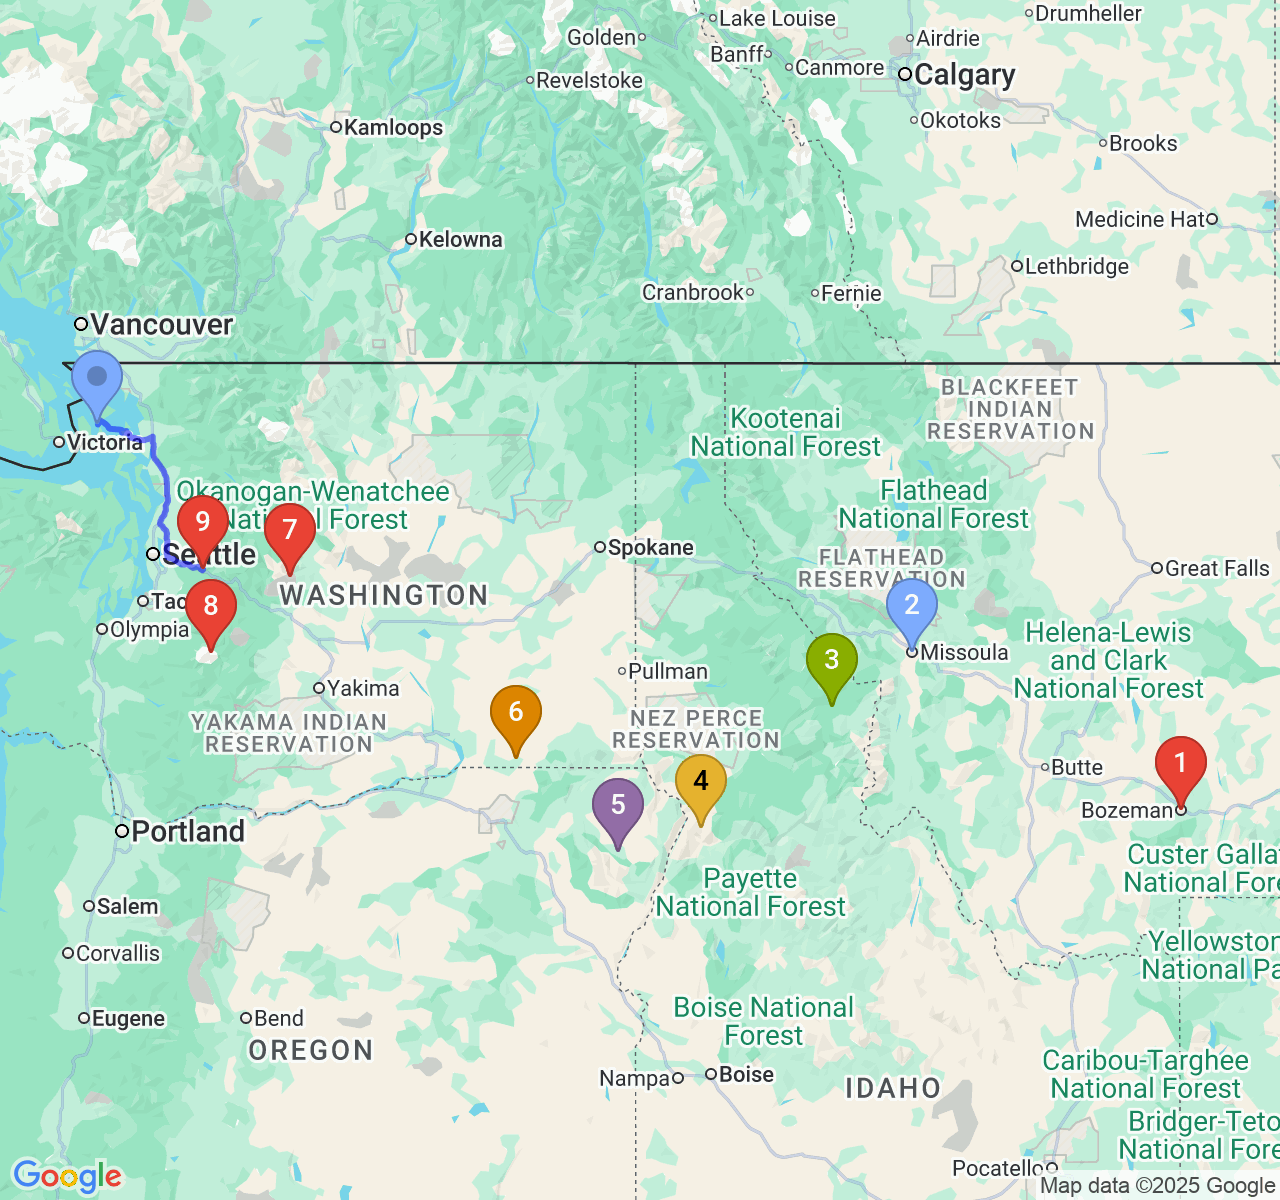
\includegraphics[width=0.5\linewidth,height=\textheight,keepaspectratio]{images/route_overview_map.png}

}

\caption{Route Overview Map}

\end{figure}%

\textbf{A Journey Through the American West}

\textbf{MONTANA}

\textbf{BOZEMAN (Aug 3-4)} - Museum of the Rockies, Yellowstone Gateway,
Elevation: 4,820 ft

\textbf{MISSOULA (Aug 5)} - Clark Fork River, University of Montana,
Elevation: 3,205 ft

\textbf{IDAHO}

\textbf{JERRY JOHNSON HOT SPRINGS (Aug 6)} - Lochsa River Valley,
Natural soaking pools, Highway 12 Scenic Byway

\textbf{MCCALL (Aug 7-8)} - Payette Lake, Payette National Forest,
Elevation: 5,021 ft

\textbf{OREGON}

\textbf{JOSEPH (Aug 9)} - Wallowa Mountains (``Alps of Oregon''),
Wallowa Lake, Elevation: 4,150 ft

\textbf{WASHINGTON}

\textbf{WALLA WALLA (Aug 10)} - Columbia River Valley, Wine Country,
Elevation: 1,001 ft

\textbf{COLUMBIA RIVER GORGE (Aug 11)} - Columbia River, Cascade Range,
Elevation: 200 ft

\textbf{SEATTLE (Aug 12-14)} - Puget Sound, Olympic \& Cascade
Mountains, Elevation: 175 ft

\subsection{Geographic Context}\label{geographic-context}

\subsubsection{Mountain Ranges
Traversed}\label{mountain-ranges-traversed}

\subsubsection{Mountain Ranges
Traversed}\label{mountain-ranges-traversed-1}

The route traverses six distinct mountain ranges, each representing
different geological formations and evolutionary histories. The Rocky
Mountains in Montana encompass the Continental Divide and extend into
the Glacier National Park region, providing the foundational geological
framework for the northern portion of the journey. The Bitterroot
Mountains along the Montana-Idaho border feature Lolo Pass and the Jerry
Johnson Hot Springs area, representing the transitional zone between
Rocky Mountain and Pacific Northwest geological provinces. The Payette
Mountains in Idaho include Brundage Mountain and extensive areas within
Payette National Forest, characterized by glacially-carved alpine
terrain.

The Wallowa Mountains in Oregon, known as the ``Alps of Oregon,''
contain the Eagle Cap Wilderness and represent some of the most
dramatically glaciated terrain in the region. The Blue Mountains
spanning Oregon and Washington provide passage through Umatilla National
Forest areas. The Cascade Range in Washington encompasses the Columbia
River Gorge and Mount Hood vicinity, representing active volcanic
geological processes.

\subsubsection{Major Rivers \& Waterways}\label{major-rivers-waterways}

Seven major waterway systems define the hydrological framework of the
route, each representing different stages in the regional drainage
evolution. The Missouri River headwaters region around Bozeman
represents the easternmost extent of the route's drainage systems. The
Clark Fork River through Missoula functions as a major tributary to the
Columbia River system and preserves extensive evidence of glacial Lake
Missoula. The Lochsa River near Jerry Johnson maintains designation as a
Wild and Scenic River, preserving natural flow characteristics through
pristine wilderness areas.

\subsubsection{Climate Zones
Experienced}\label{climate-zones-experienced}

The route crosses five distinct climate zones, each supporting different
ecosystems and reflecting varying geographical influences. Continental
climate conditions in Montana feature dry summers and cold winters,
reflecting the region's position within the North American continental
interior and distance from maritime influences. Maritime-influenced
continental climate in Idaho provides moderate four-season patterns with
increased precipitation from Pacific air masses penetrating inland
through mountain gaps. High desert climate in eastern Oregon creates
hot, dry summer conditions with minimal precipitation, reflecting the
rain shadow effects of surrounding mountain ranges. Mediterranean
climate around Walla Walla supports wine-growing conditions through
warm, dry summers and mild, wet winters similar to Mediterranean Basin
climates. Temperate oceanic climate in western Washington produces mild,
wet winters and moderate summers, reflecting direct maritime influences
from Pacific Ocean air masses.

\subsubsection{Elevation Profile}\label{elevation-profile}

\begin{figure}[H]

{\centering \pandocbounded{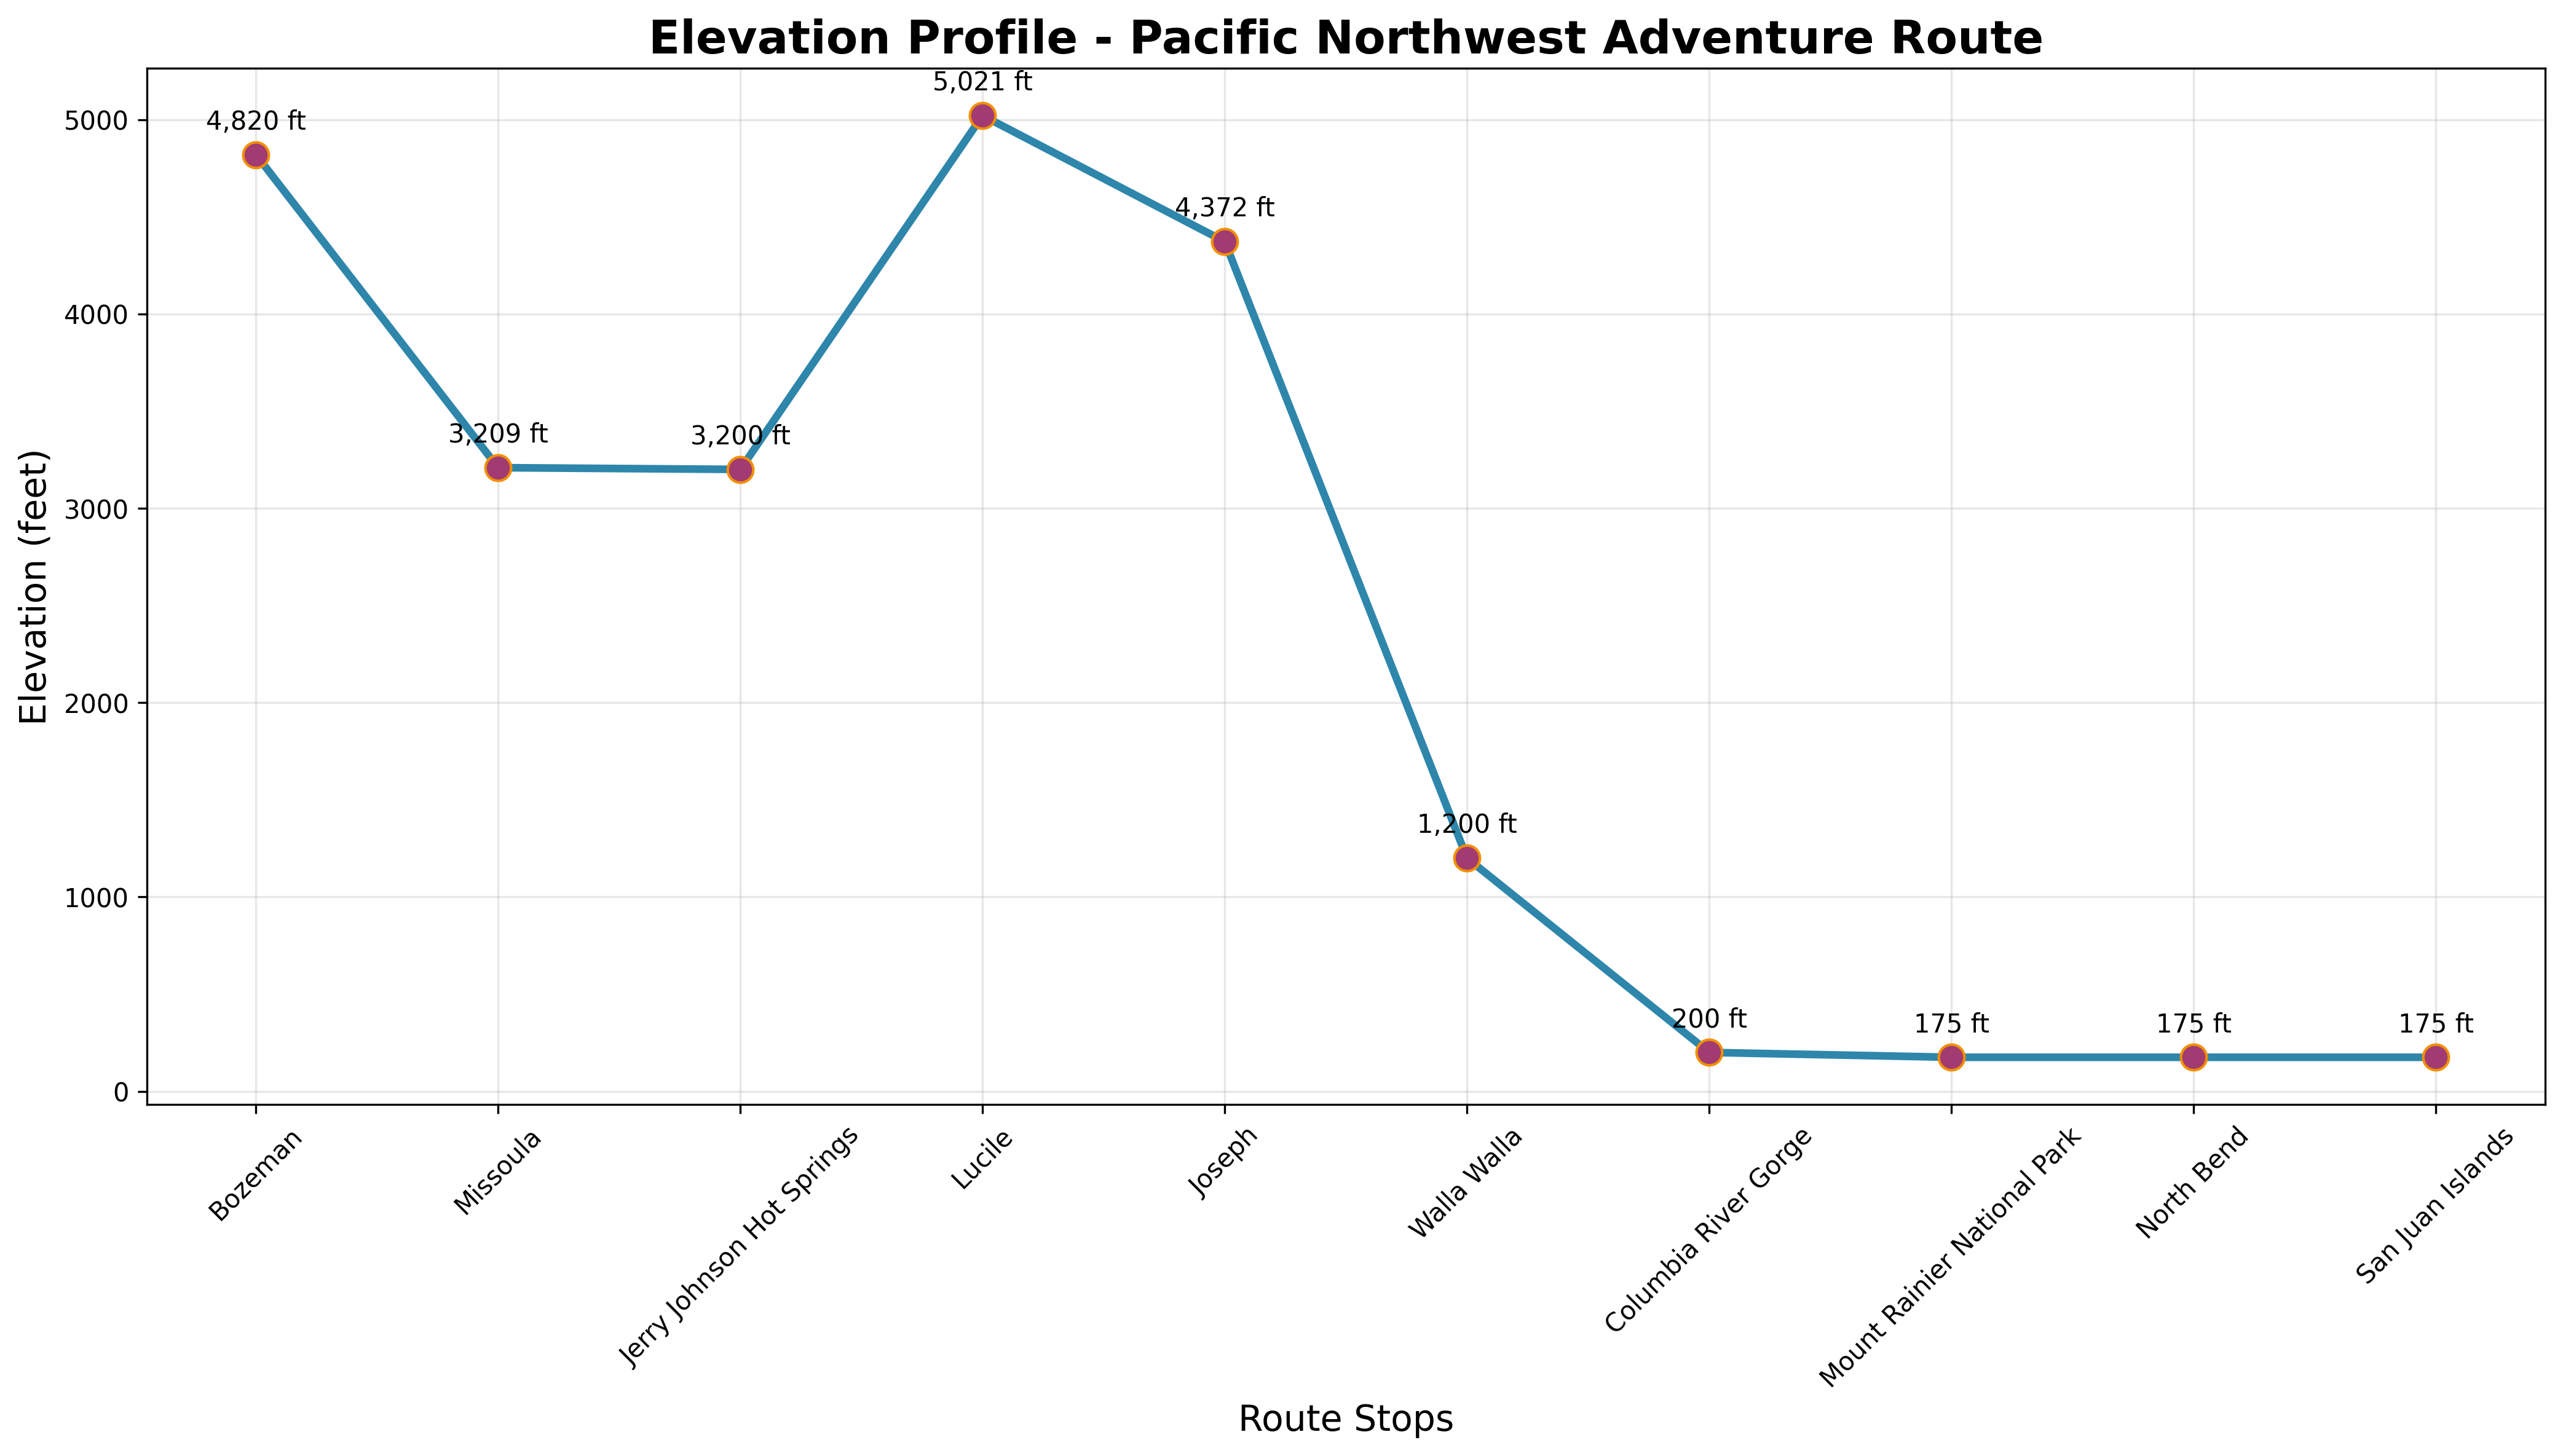
\includegraphics[keepaspectratio]{images/elevation_profile.png}}

}

\caption{Elevation Profile}

\end{figure}%

The route traverses dramatic elevation changes from Seattle's sea level
(175 ft) to McCall's mountain elevation (5,021 ft), crossing multiple
climate zones and terrain types.

\newpage

\section{Route Summary}\label{route-summary}

\textbf{Travelers:} Gil, Camila, Aviv, and Smadar (Aviv \& Smadar
departing Seattle 8/12)\\
\textbf{Duration:} August 3-14, 2025\\
\textbf{Route:} Montana → Idaho → Oregon → Washington

\begin{longtable}[]{@{}
  >{\raggedright\arraybackslash}p{(\linewidth - 10\tabcolsep) * \real{0.1216}}
  >{\raggedright\arraybackslash}p{(\linewidth - 10\tabcolsep) * \real{0.1351}}
  >{\raggedright\arraybackslash}p{(\linewidth - 10\tabcolsep) * \real{0.1216}}
  >{\raggedright\arraybackslash}p{(\linewidth - 10\tabcolsep) * \real{0.1892}}
  >{\raggedright\arraybackslash}p{(\linewidth - 10\tabcolsep) * \real{0.2162}}
  >{\raggedright\arraybackslash}p{(\linewidth - 10\tabcolsep) * \real{0.2162}}@{}}
\toprule\noalign{}
\begin{minipage}[b]{\linewidth}\raggedright
\textbf{Leg}
\end{minipage} & \begin{minipage}[b]{\linewidth}\raggedright
\textbf{From}
\end{minipage} & \begin{minipage}[b]{\linewidth}\raggedright
\textbf{To}
\end{minipage} & \begin{minipage}[b]{\linewidth}\raggedright
\textbf{Distance}
\end{minipage} & \begin{minipage}[b]{\linewidth}\raggedright
\textbf{Drive Time}
\end{minipage} & \begin{minipage}[b]{\linewidth}\raggedright
\textbf{Highlights}
\end{minipage} \\
\midrule\noalign{}
\endhead
\bottomrule\noalign{}
\endlastfoot
1 & Bozeman & Missoula & 202 mi & 2h 58m & Montana exploration \\
2 & Missoula & Jerry Johnson Hot Springs & 66 mi & 1h 20m & Scenic
highway route \\
3 & Jerry Johnson & McCall & 190 mi & 3h 49m & Mountain lakes \&
forests \\
4 & McCall & Joseph & 166 mi & 4h 19m & Wallowa Mountains \\
5 & Joseph & Walla Walla & 109 mi & 2h 11m & Wine country arrival \\
6 & Walla Walla & Columbia River Gorge & 205 mi & 3h 37m & Scenic gorge
drive \\
7 & Columbia River Gorge & Seattle & 110 mi & 2h 10m & Final
destination \\
\end{longtable}

\textbf{Total Distance:} 1,049 miles\\
\textbf{Total Driving Time:} 20.4 hours\\
\textbf{Average Daily Drive:} 2.9 hours

\newpage

\section{Hotel Walking Maps - Quick Reference
Guide}\label{hotel-walking-maps---quick-reference-guide}

This section provides full-page spreads of all walking vicinity maps for
easy reference throughout your trip. Each map shows everything within a
30-minute walk of your hotel using high-resolution satellite imagery
with street overlays.

\newpage

\subsection{Bozeman, Montana Walking
Map}\label{bozeman-montana-walking-map}

\textbf{Kimpton Armory Hotel \textbar{} August 3-4}

\begin{figure}[H]

{\centering \pandocbounded{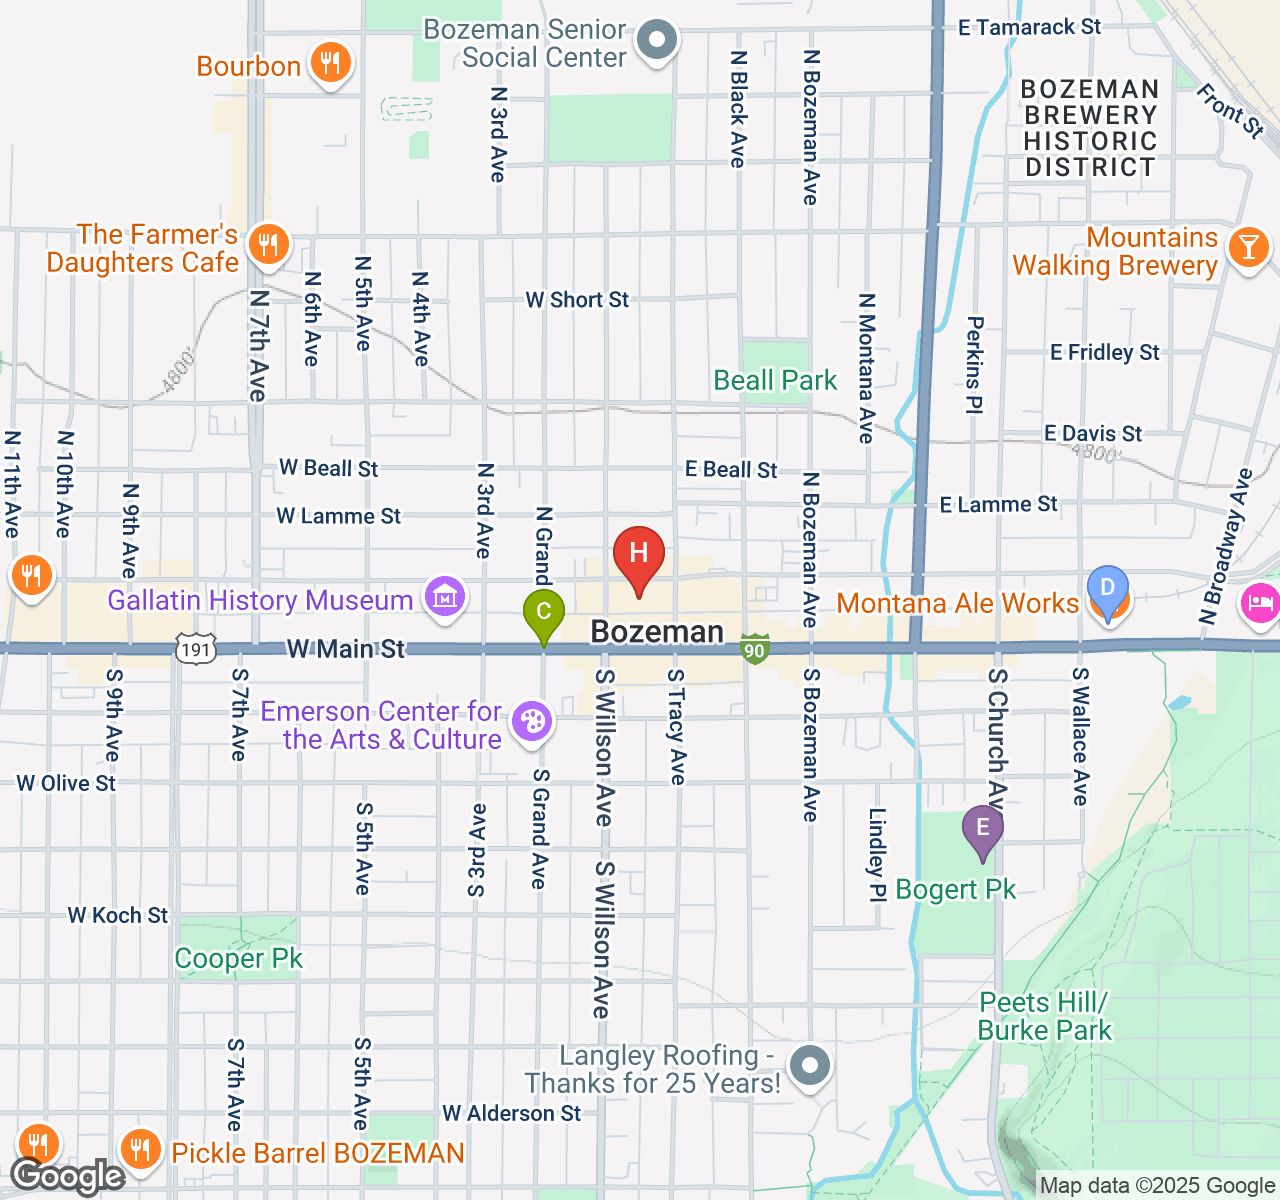
\includegraphics[keepaspectratio]{images/bozeman_mt_walking_map.png}}

}

\caption{Bozeman Walking Vicinity Map}

\end{figure}%

\textbf{Hotel:} Kimpton Armory Hotel \textbar{} 24 W Mendenhall St
\textbar{} (406) 551-7000

\textbf{Within Walking Distance:} - Main Street Historic District -
Historic downtown core with shops and galleries - Wild Crumb Bakery -
European artisan breads and sourdough culture - Great Harvest Bread
Co.~- Fresh-milled Montana wheat breads - Blackbird Kitchen - Wood-fired
Argentine-style asado and lamb - Montana State University Campus -
Historic university grounds - Bogert Park - Green space with trails and
recreation - Local breweries and craft beer scene

\newpage

\subsection{Missoula, Montana Walking
Map}\label{missoula-montana-walking-map}

\textbf{AC Hotel Missoula Downtown \textbar{} August 5}

\begin{figure}[H]

{\centering \pandocbounded{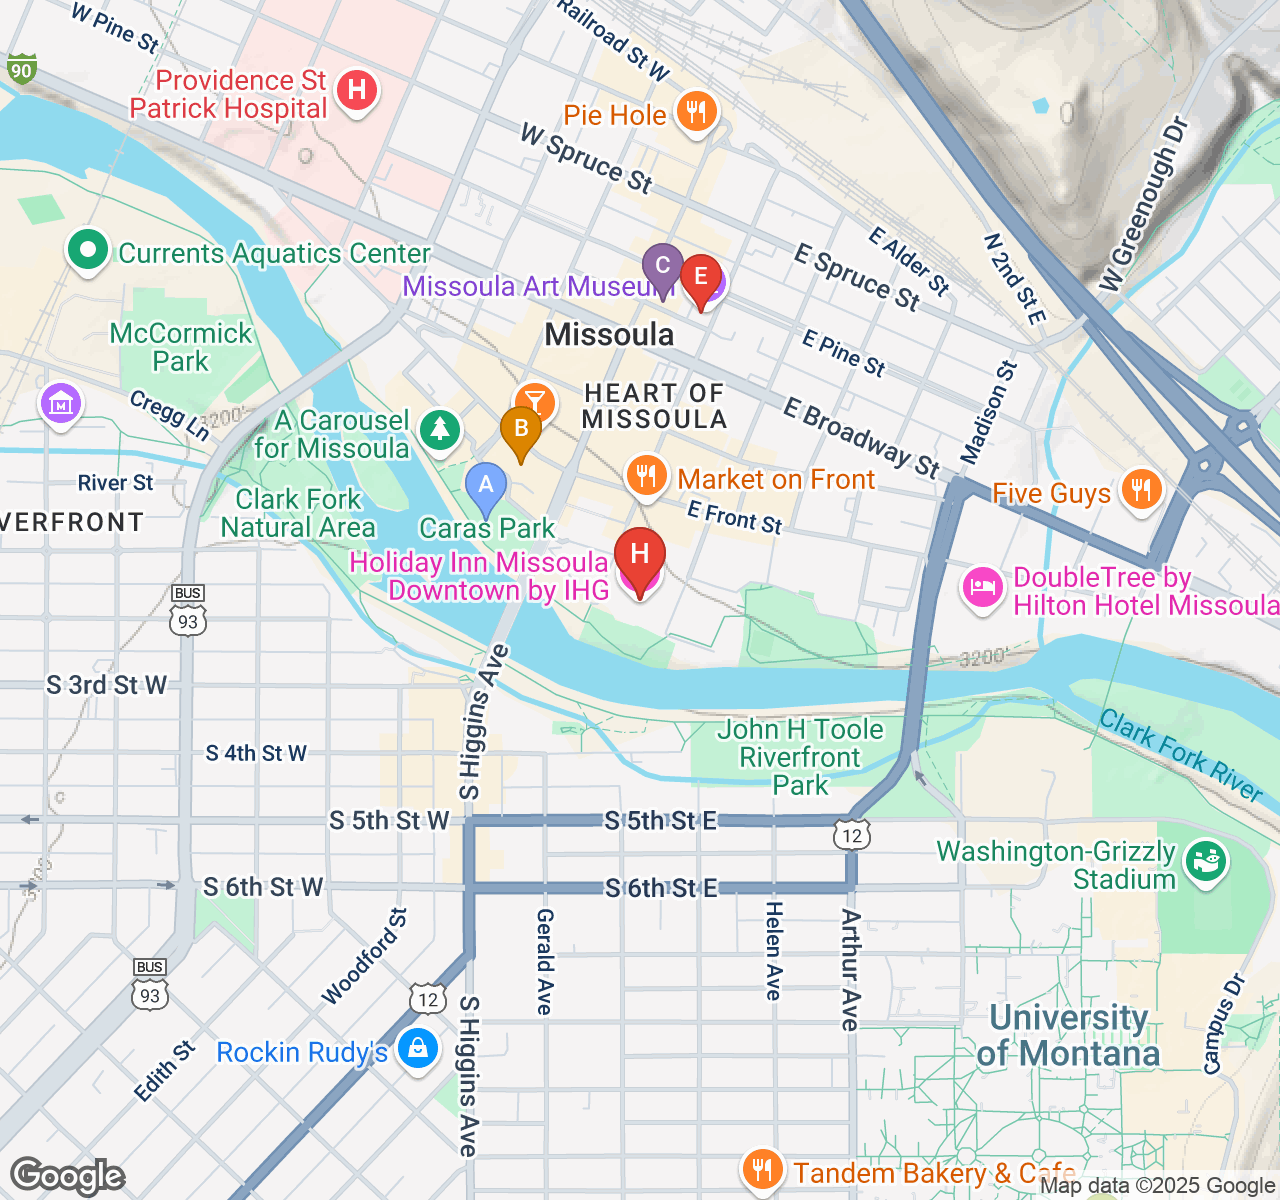
\includegraphics[keepaspectratio]{images/missoula_mt_walking_map.png}}

}

\caption{Missoula Walking Vicinity Map}

\end{figure}%

\textbf{Hotel:} AC Hotel Missoula Downtown \textbar{} 200 S Pattee St
\textbar{} (406) 532-3344

\textbf{Within Walking Distance:} - Clark Fork Riverfront Trail - Scenic
riverside walking path - University of Montana Campus - Historic campus
with museums - Downtown Historic District - Vibrant downtown with local
culture - Le Petit Outre - French pastries and European breads - Plonk
Wine Bar - Argentine-inspired cuisine and wine - Higgins Avenue Bridge -
Iconic bridge with river views - Local art galleries and cultural sites

\newpage

\subsection{Lucile, Idaho Walking Map}\label{lucile-idaho-walking-map}

\textbf{Steelhead Lodge \textbar{} August 7-8}

\begin{figure}[H]

{\centering \pandocbounded{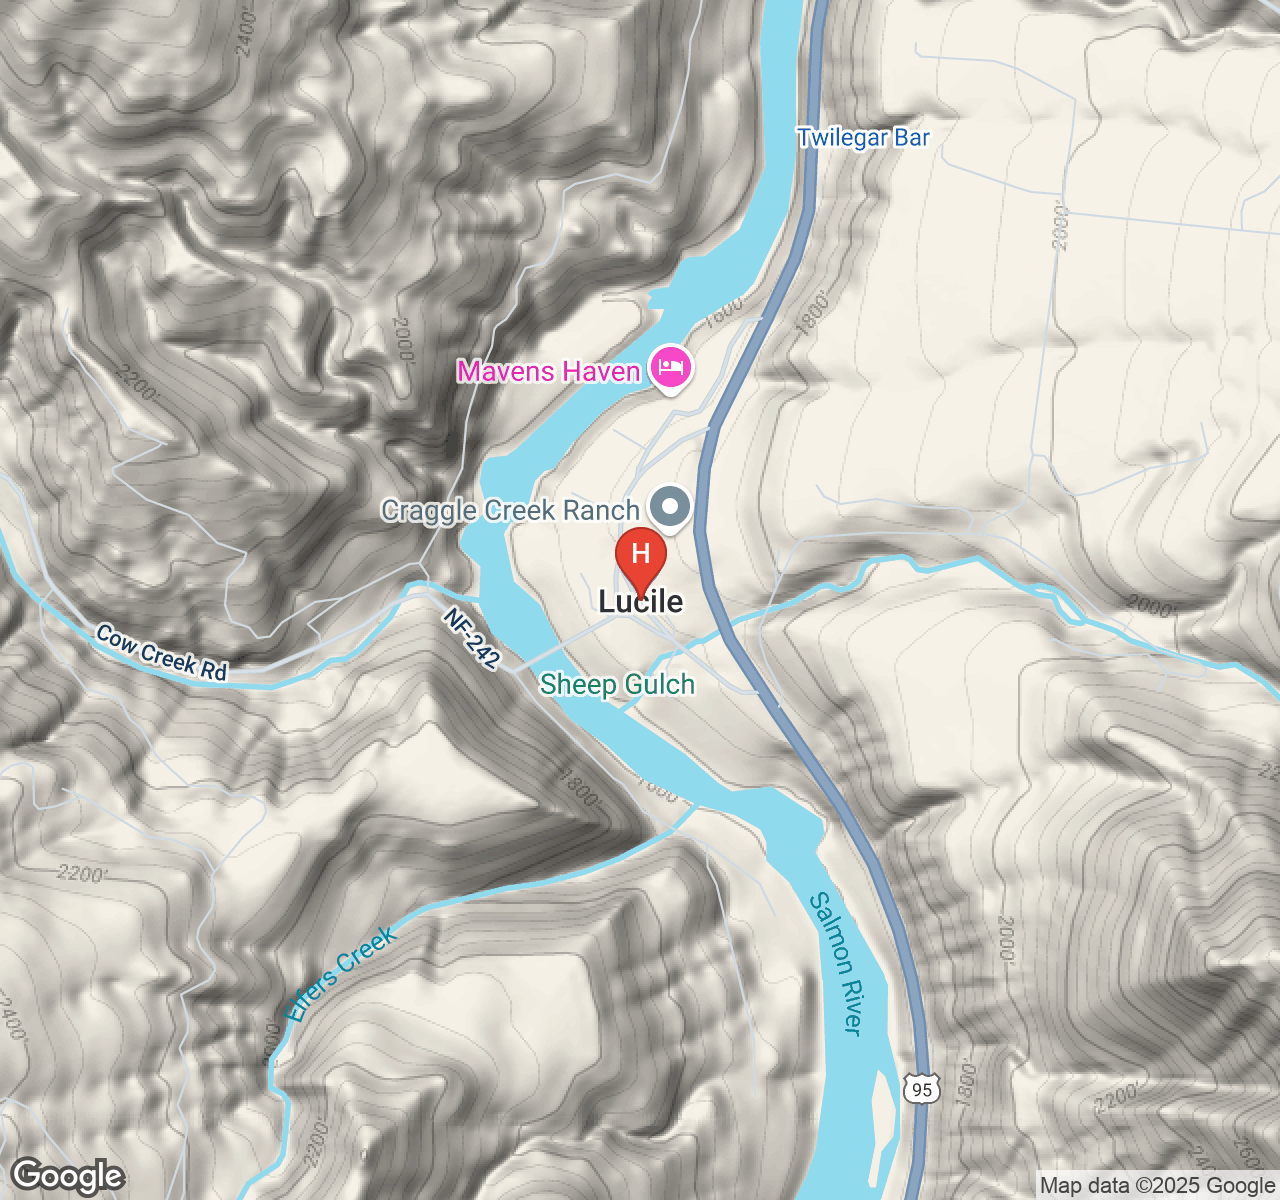
\includegraphics[keepaspectratio]{images/lucile_id_walking_map.png}}

}

\caption{Lucile Walking Vicinity Map}

\end{figure}%

\textbf{Lodge:} Steelhead Lodge \textbar{} Lucile, ID \textbar{} (208)
628-3647

\textbf{Within Walking Distance:} - Salmon River Access - World-class
fishing and river activities - River Canyon Overlook - Spectacular views
of Salmon River Canyon - Historic Mining Sites - Gold rush era remnants
and interpretive sites - Fishing Guide Services - Professional salmon
fishing guide headquarters - Lodge Marina - Boat launch and jet boat
tour departures

\newpage

\subsection{Twin Peaks Filming Locations
Map}\label{twin-peaks-filming-locations-map}

\textbf{North Bend \& Snoqualmie \textbar{} August 12th}

\begin{figure}[H]

{\centering \pandocbounded{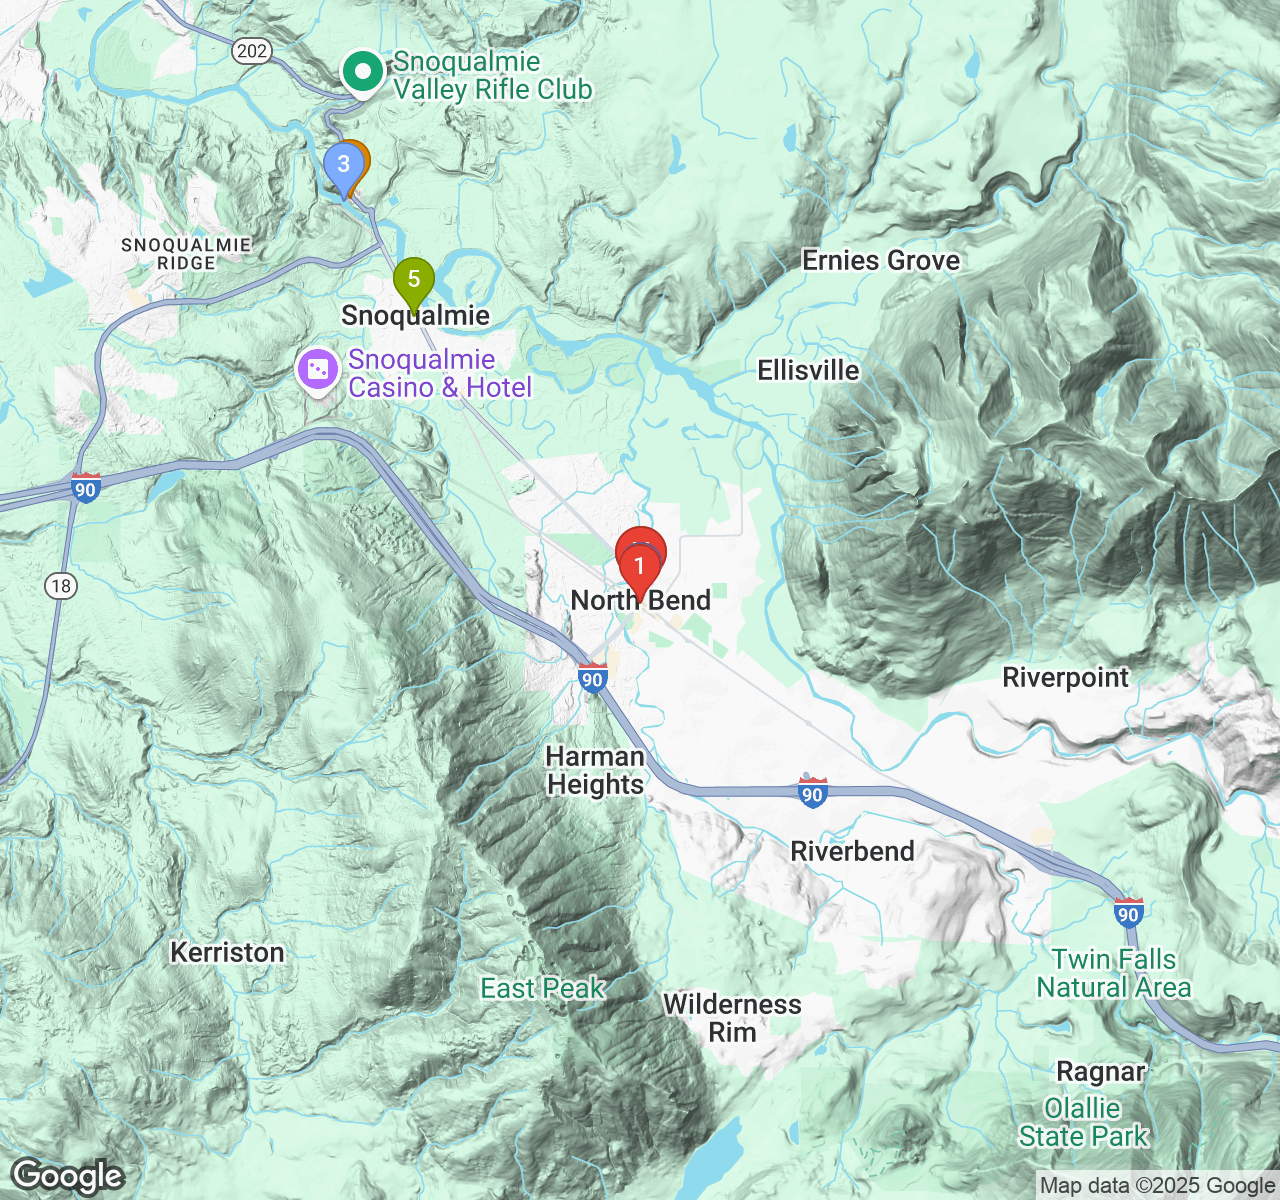
\includegraphics[keepaspectratio]{images/twin_peaks_wa_recommendations_map.png}}

}

\caption{Twin Peaks Filming Locations Map}

\end{figure}%

\textbf{Filming Sites Tour:} - Twede's Cafe (Double R Diner) - Interior
scenes and Agent Cooper's booth - Salish Lodge (Great Northern Hotel) -
Exterior establishing shots - Snoqualmie Falls - Opening credits
waterfall - North Bend Theatre - Town exterior scenes - Snoqualmie Depot
- Railway background scenes

\newpage

\subsection{Orcas Island Walking Map}\label{orcas-island-walking-map}

\textbf{Round House Suite, Rosario Village \textbar{} August 13th}

\begin{figure}[H]

{\centering \pandocbounded{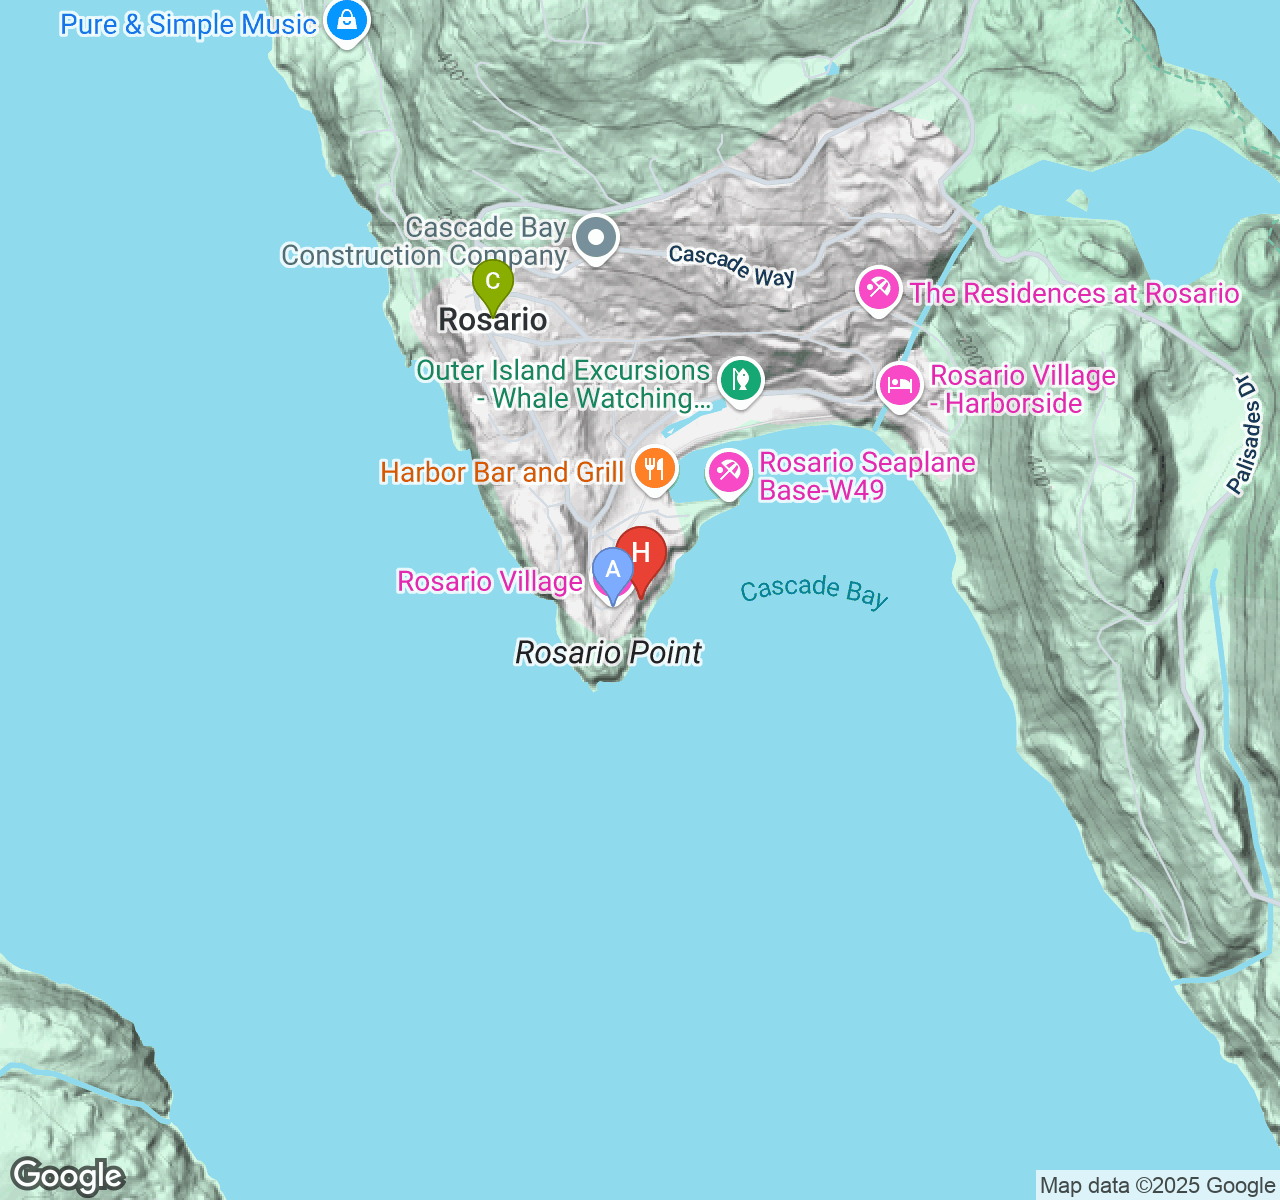
\includegraphics[keepaspectratio]{images/orcas_island_wa_walking_map.png}}

}

\caption{Orcas Island Walking Vicinity Map}

\end{figure}%

\textbf{Accommodation:} Round House Suite, Rosario Village \textbar{}
1400 Rosario Rd \textbar{} (360) 376-2222

\textbf{Within Walking Distance:} - Kayak Launch Point - Direct access
to peak orca viewing waters - Rosario Village Marina - Historic mansion
and spa facilities - Eastsound Village Center - Island shopping and
dining - Olga Orca Viewing - Historical orca sighting lookout points -
Buck Bay Shellfish Farm - Fresh oyster harvesting experience

\newpage

\subsection{San Juan Island Walking
Map}\label{san-juan-island-walking-map}

\textbf{Friday Harbor Area \textbar{} August 14th Morning}

\begin{figure}[H]

{\centering \pandocbounded{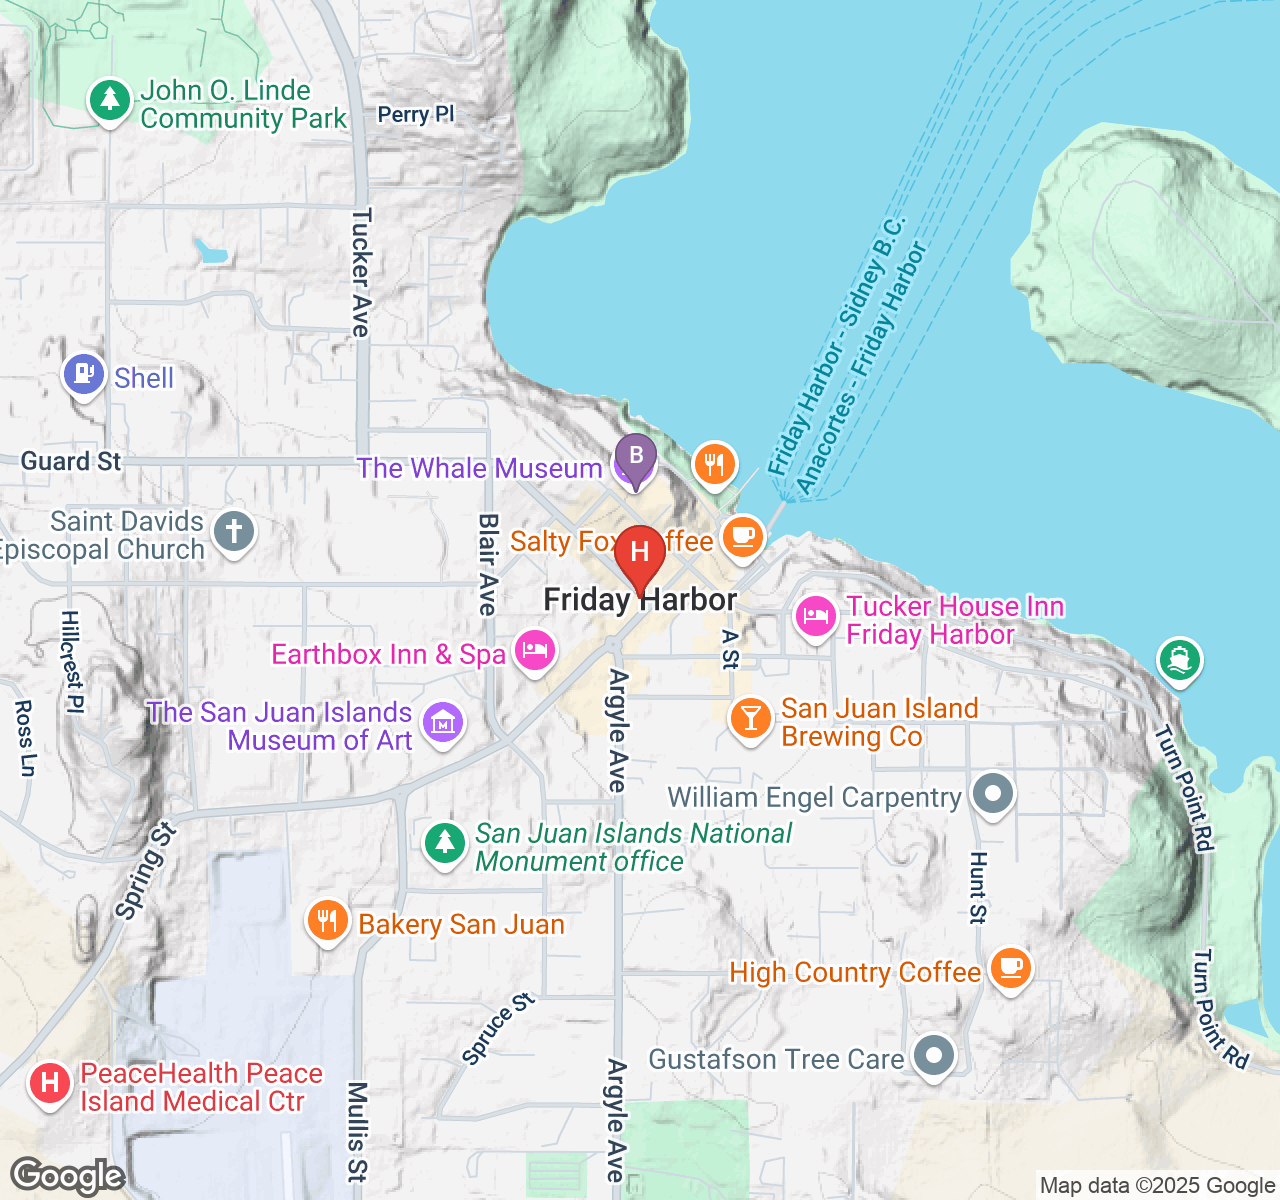
\includegraphics[keepaspectratio]{images/san_juan_island_wa_walking_map.png}}

}

\caption{San Juan Island Walking Vicinity Map}

\end{figure}%

\textbf{Ferry Hub:} Friday Harbor \textbar{} Ferry Terminal

\textbf{Within Walking Distance:} - The Whale Museum - Marine biology
research and orca education - Friday Harbor Downtown - Island shopping
and dining - Ferry Terminal - Inter-island transportation hub - Roche
Harbor - Historic lime manufacturing village - Lime Kiln Point State
Park - Premier land-based whale watching

\newpage

\subsection{Lopez Island Walking Map}\label{lopez-island-walking-map}

\textbf{Lopez Village \textbar{} August 14th Afternoon}

\begin{figure}[H]

{\centering \pandocbounded{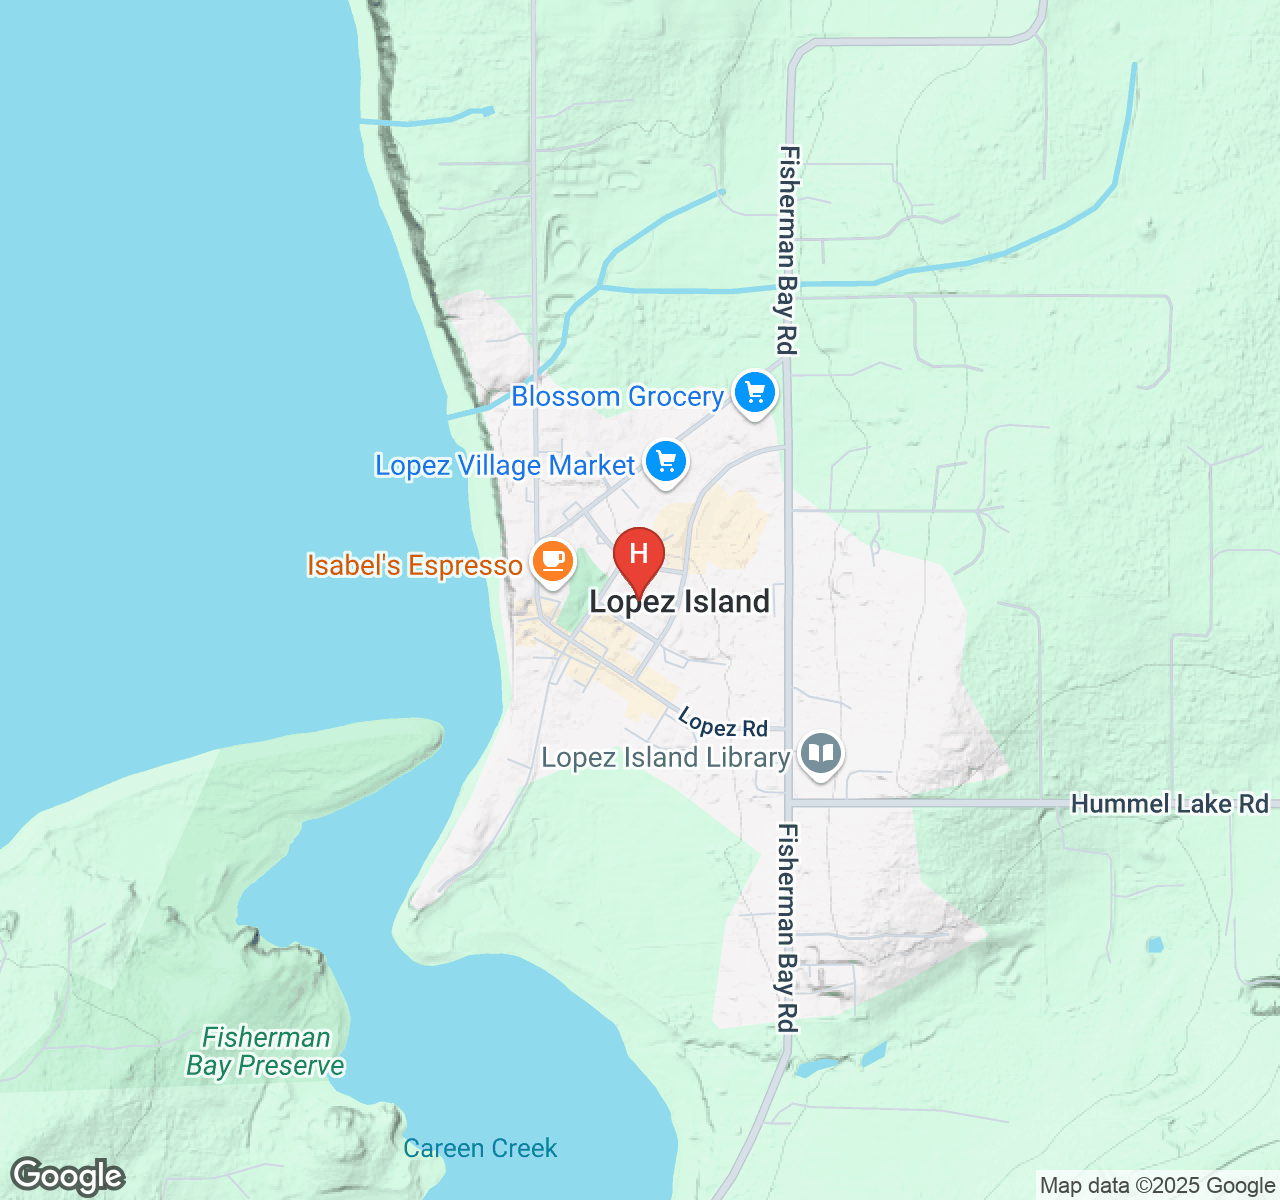
\includegraphics[keepaspectratio]{images/lopez_island_wa_walking_map.png}}

}

\caption{Lopez Island Walking Vicinity Map}

\end{figure}%

\textbf{Art Studios Tour Route:} - Chimera Gallery - Multi-media
sculptural works and installations - Lopez Island Pottery - Ceramic
artists working with local clay deposits - Islands' Sounder Building -
Historic newspaper building converted to studios - Textile Arts Studios
- Pacific Northwest materials and traditional techniques - Ferry
Terminal - Final departure point to mainland

\newpage

\subsection{Joseph, Oregon Walking Map}\label{joseph-oregon-walking-map}

\textbf{The Jennings Hotel \textbar{} August 9}

\begin{figure}[H]

{\centering \pandocbounded{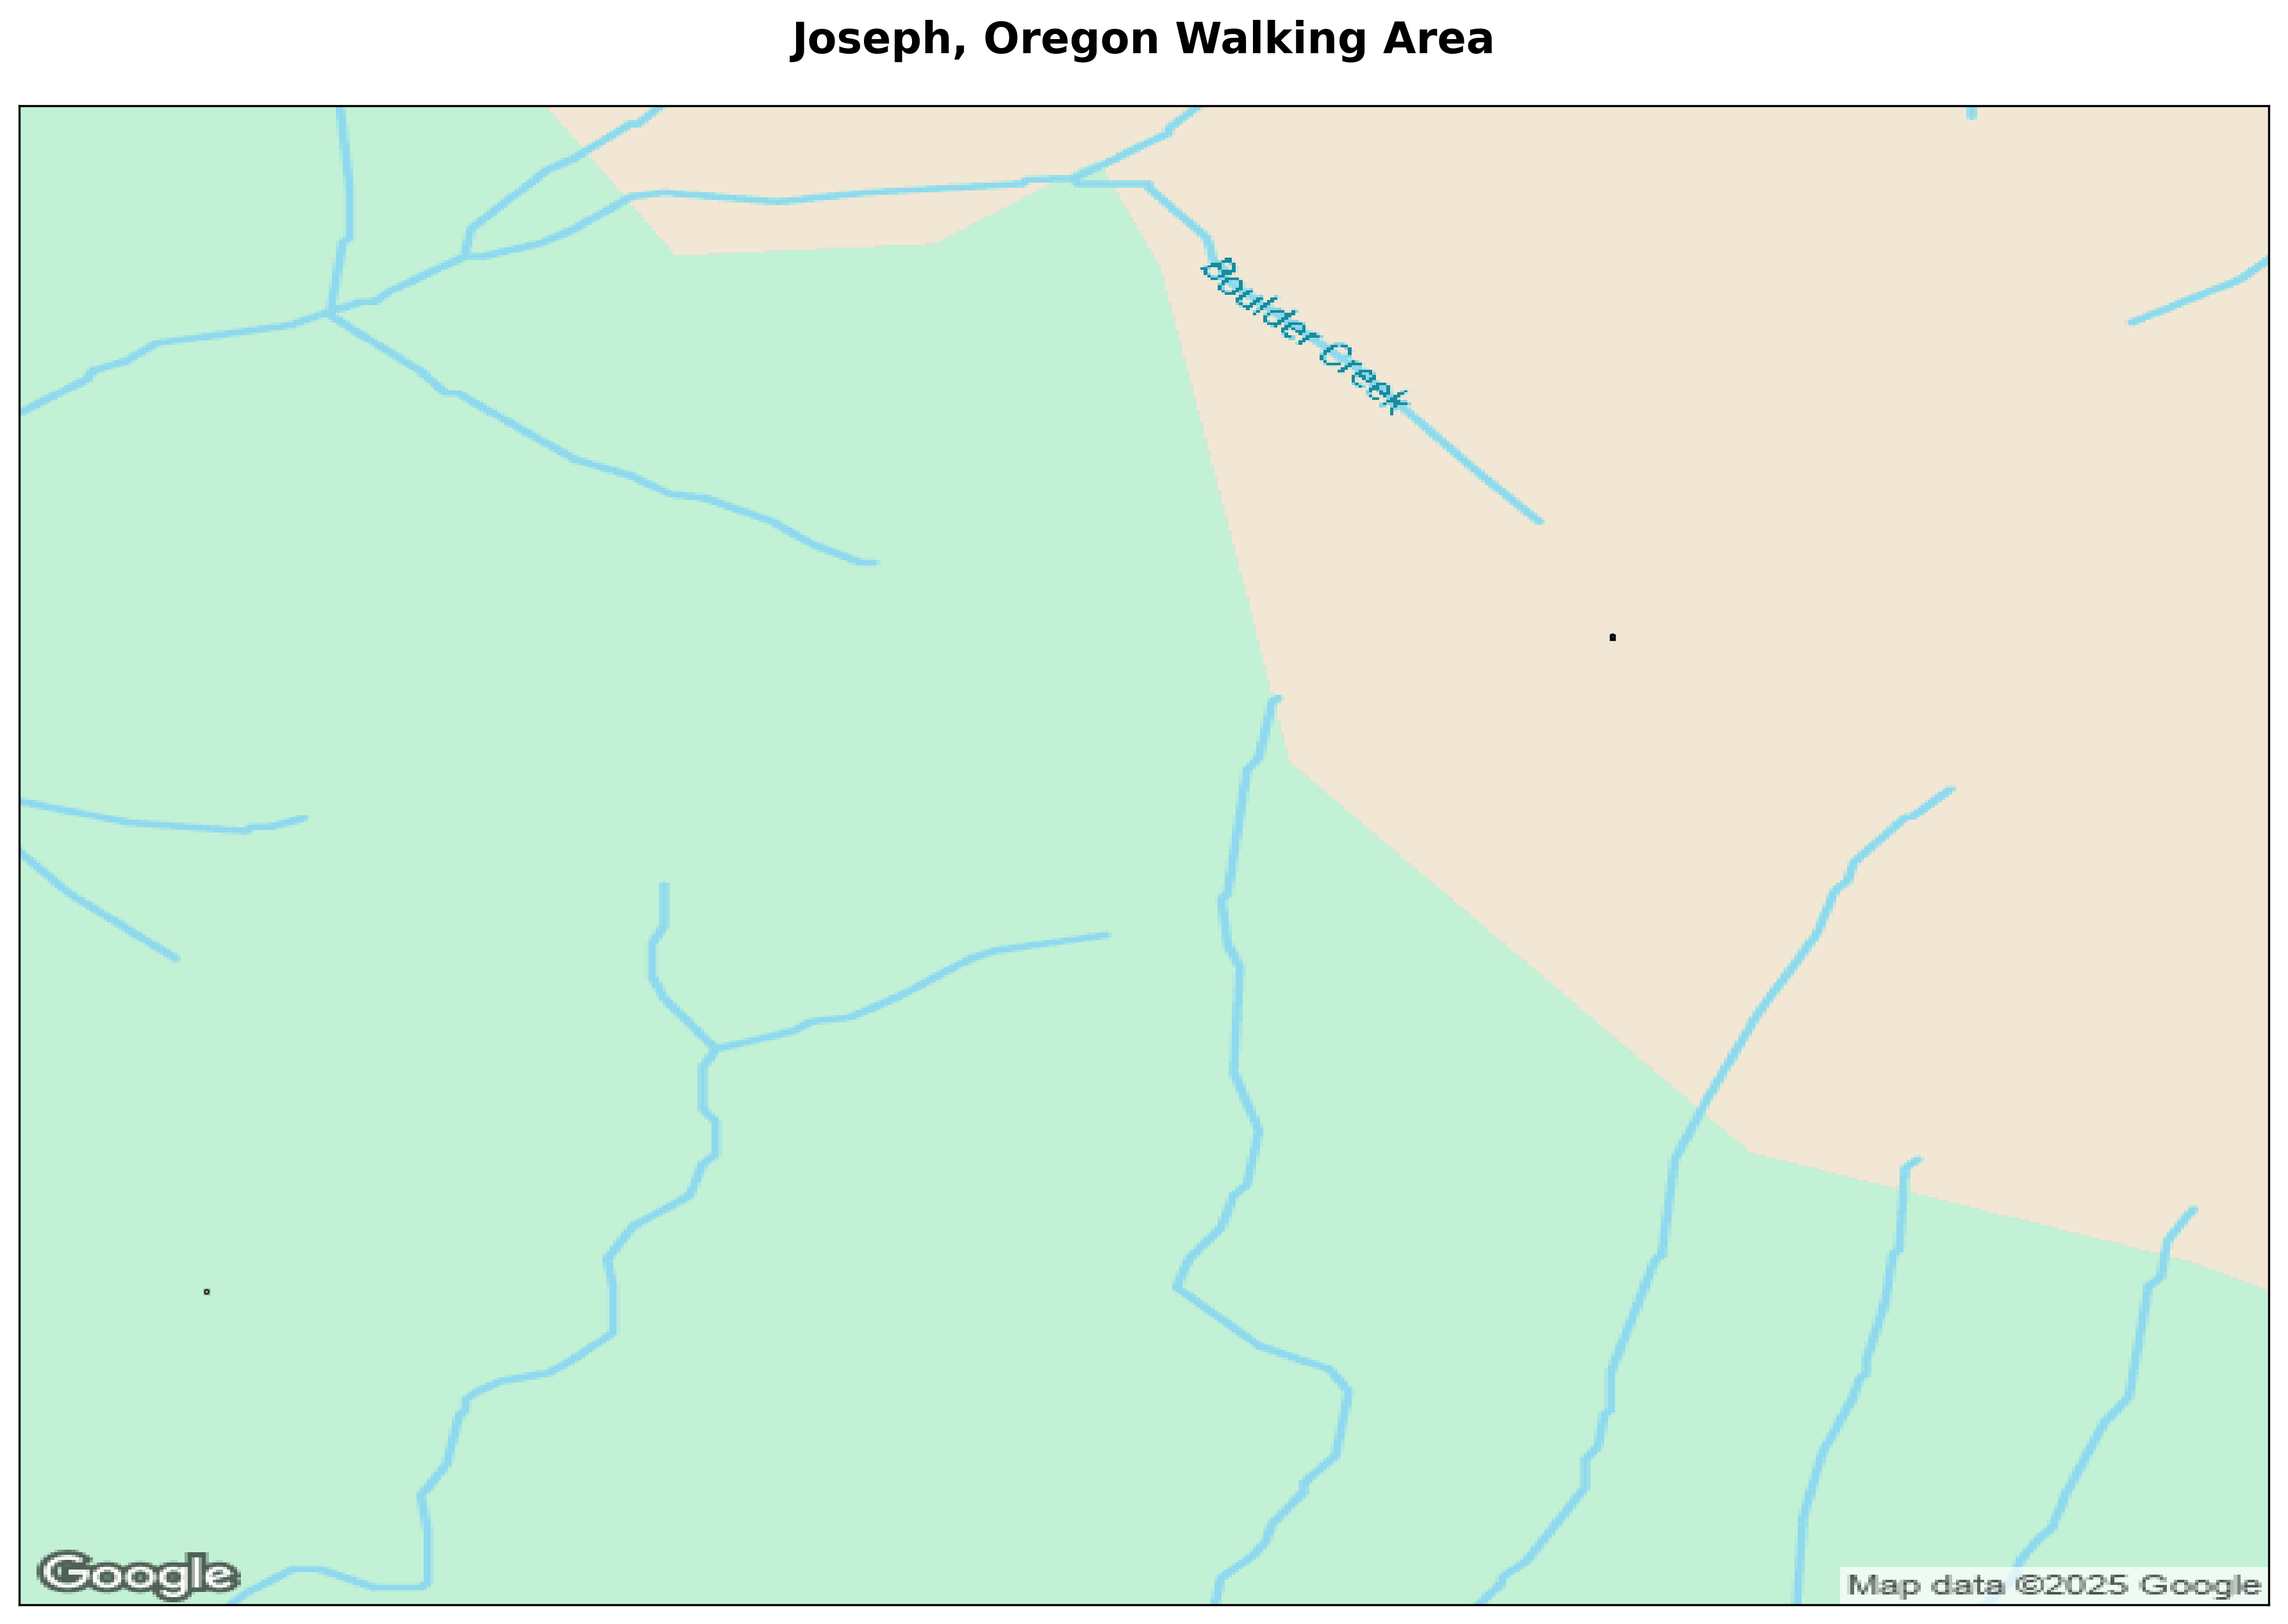
\includegraphics[keepaspectratio]{images/joseph_or_walking_map.png}}

}

\caption{Joseph Walking Vicinity Map}

\end{figure}%

\textbf{Hotel:} The Jennings Hotel \textbar{} 100 Main St \textbar{}
(541) 432-0230

\textbf{Within Walking Distance:} - Valley Bronze of Oregon - Working
bronze foundry with public access - Embers Brewhouse - Local brewery
with mountain atmosphere - Main Street Historic District - Authentic
western town character - Lear's Main Street Grill - Local dining and
mountain cuisine - Town Park - Community green space and recreation -
Artist studios and galleries throughout downtown - Wallowa Mountains
viewpoints and photo opportunities

\newpage

\subsection{Lostine, Oregon Walking
Map}\label{lostine-oregon-walking-map}

\textbf{Day Trip from Joseph \textbar{} August 9}

\begin{figure}[H]

{\centering \pandocbounded{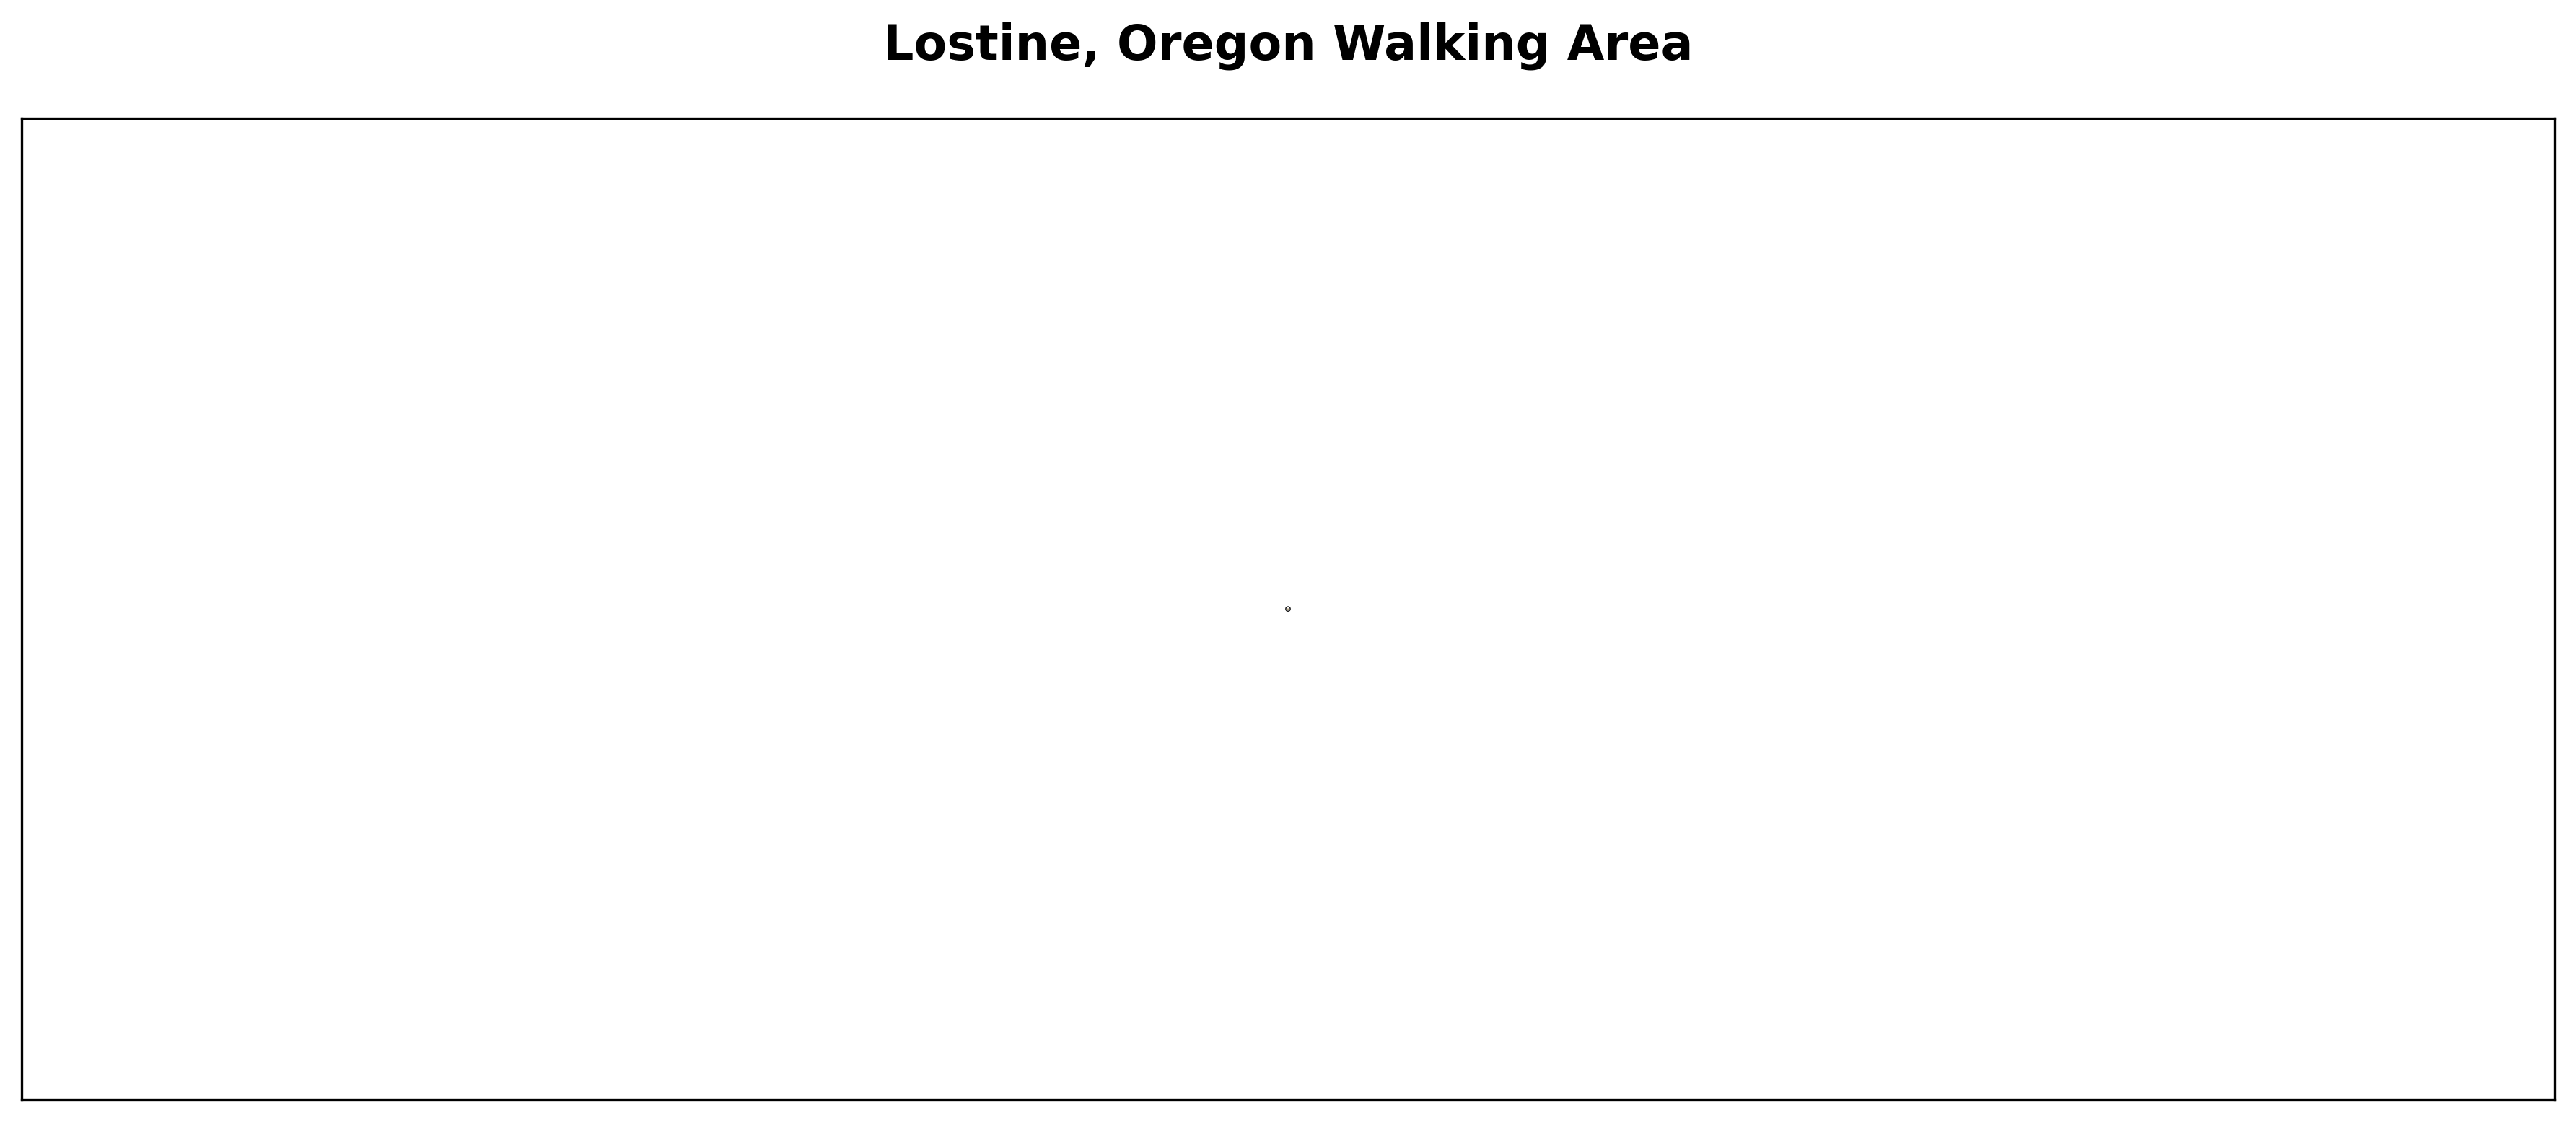
\includegraphics[keepaspectratio]{images/lostine_oregon_town_walking_map.png}}

}

\caption{Lostine Walking Vicinity Map}

\end{figure}%

\textbf{Distance from Joseph:} 8 miles north \textbar{} \textbf{Drive
Time:} 12 minutes

\textbf{Within Walking Distance:} - M. Crow \& Co.~General Store -
Internationally renowned design destination - Lostine Tavern - Authentic
Western atmosphere and community hub - Historic Methodist Church -
Community cultural center - Main Street Historic Buildings - Original
homestead architecture - Lostine River Access - Scenic river walks and
fishing - Eagle Cap Wilderness Trailheads - Alpine hiking access -
Working cattle ranches - Authentic ranching heritage

\newpage

\subsection{Walla Walla, Washington Walking
Map}\label{walla-walla-washington-walking-map}

\textbf{Eritage Resort \textbar{} August 10}

\begin{figure}[H]

{\centering \pandocbounded{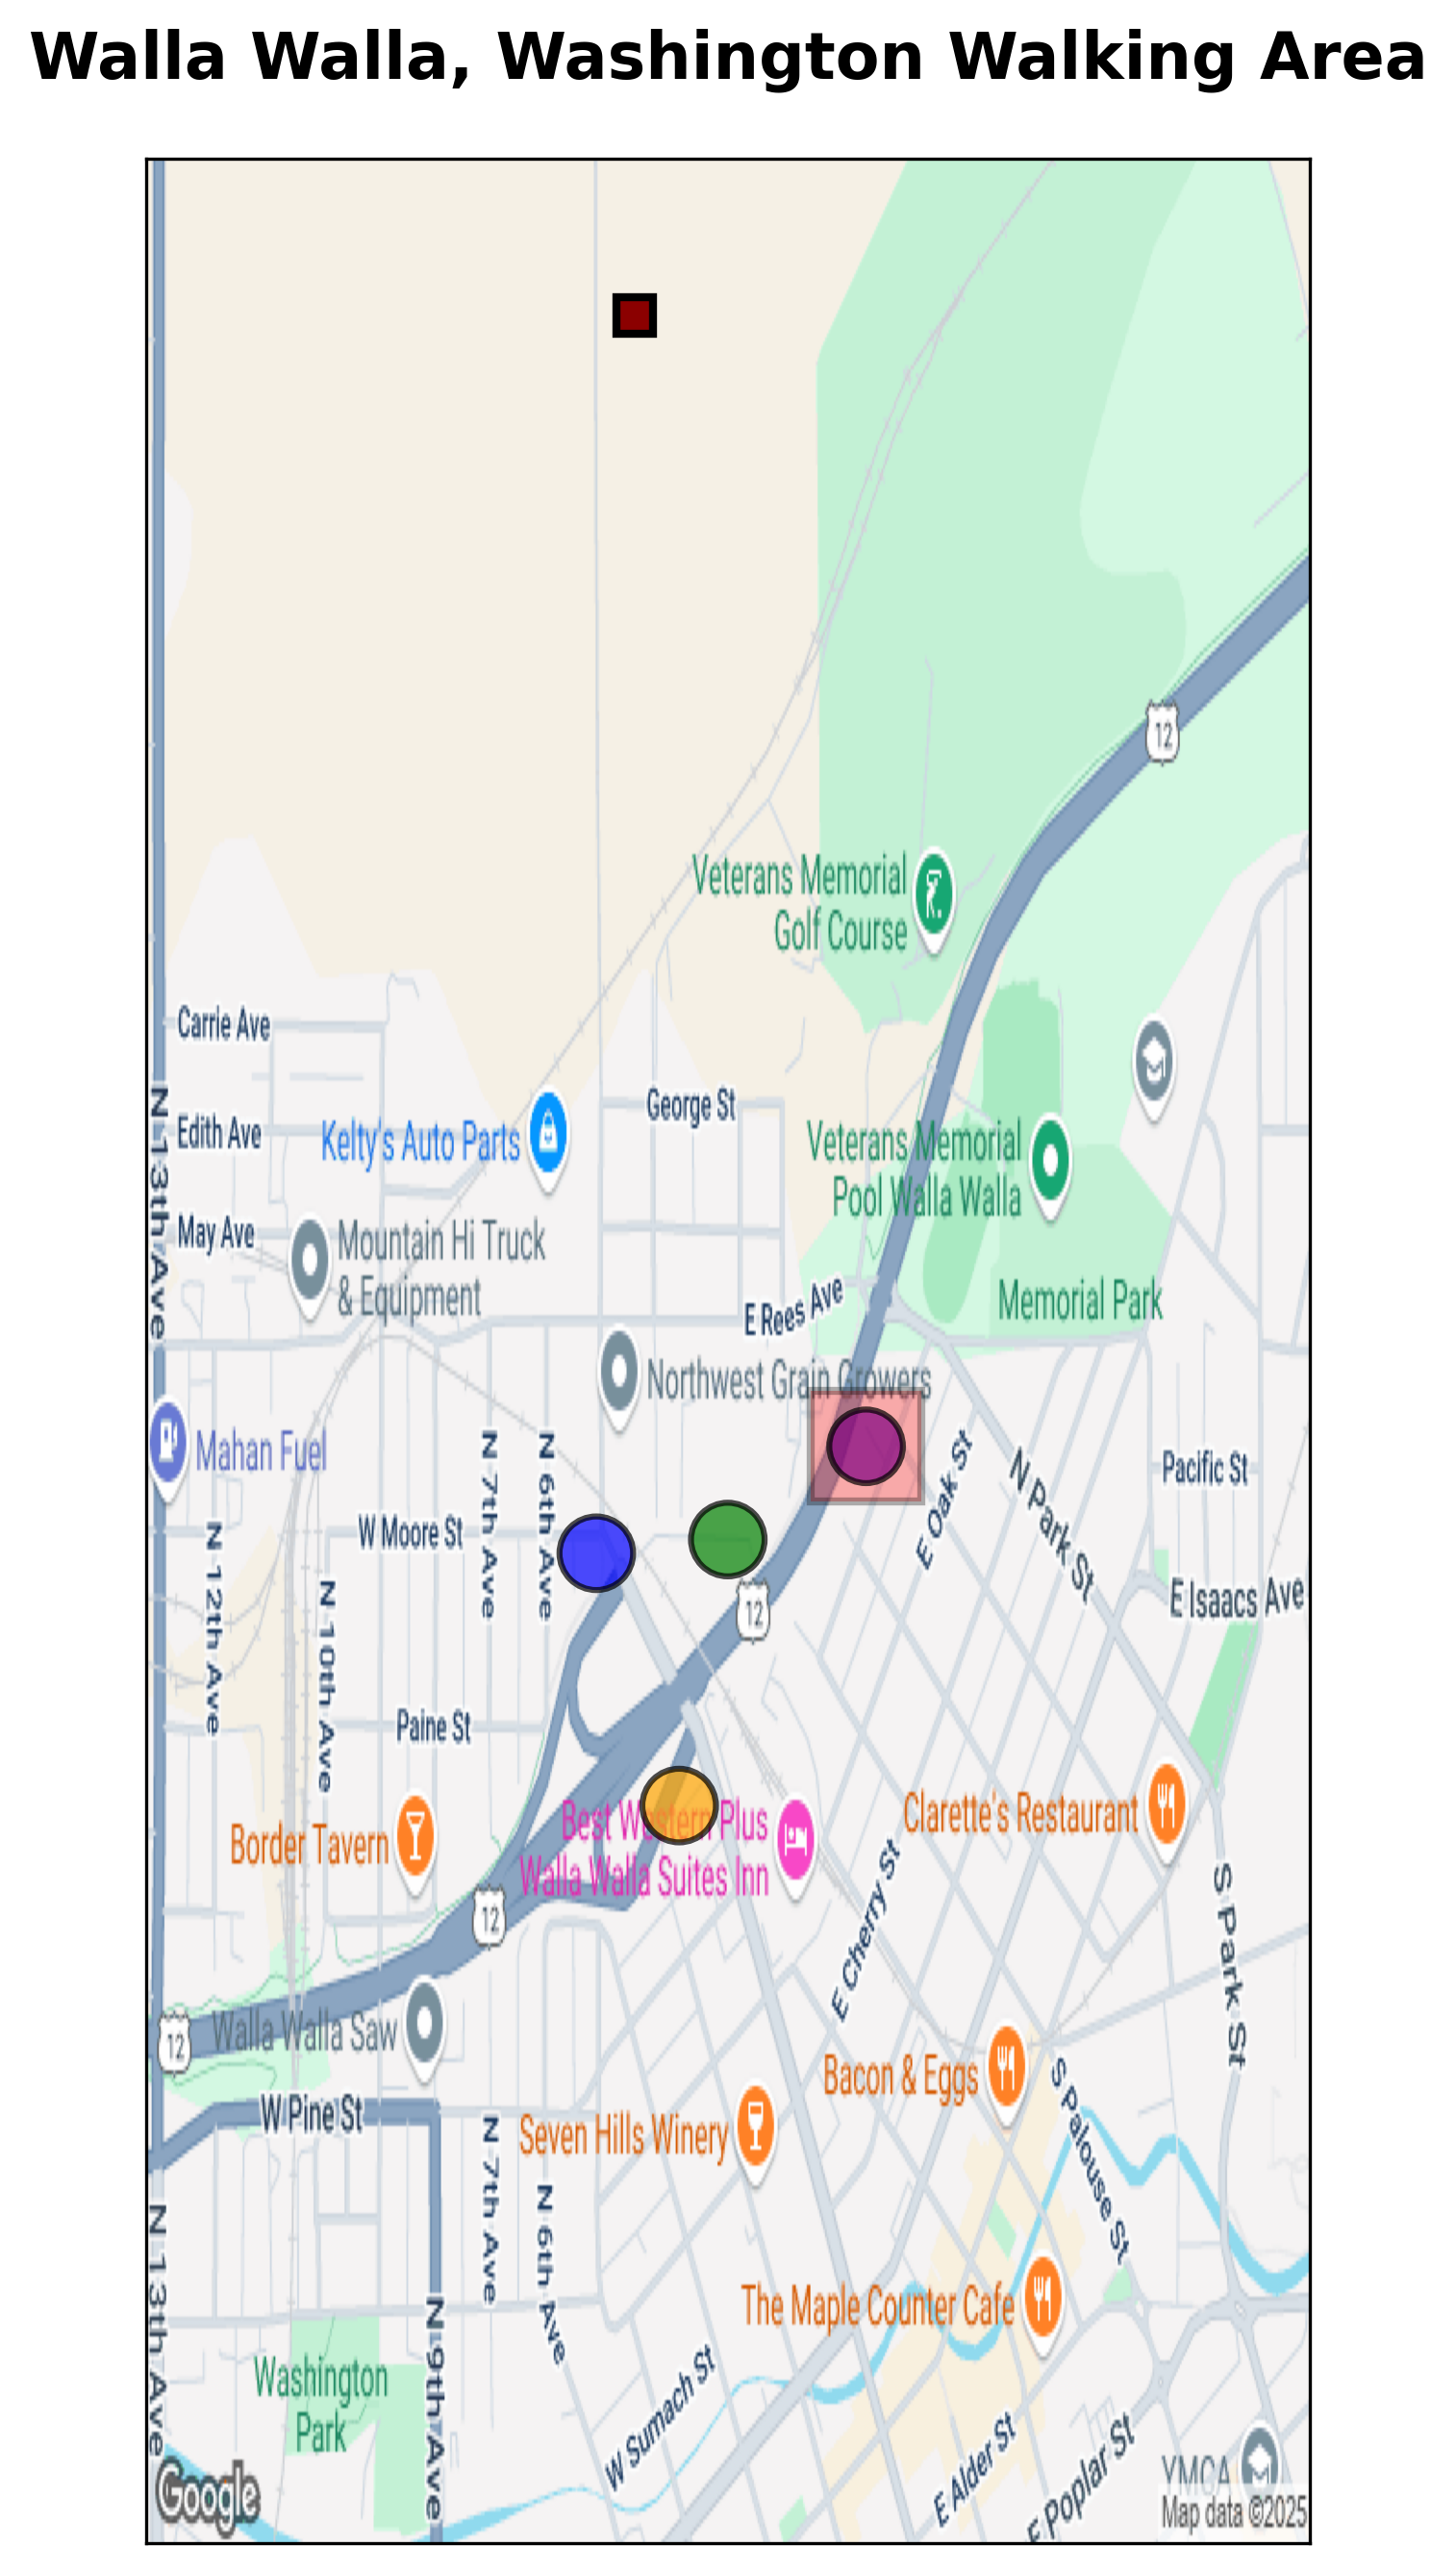
\includegraphics[keepaspectratio]{images/walla_walla_wa_walking_map.png}}

}

\caption{Walla Walla Walking Vicinity Map}

\end{figure}%

\textbf{Hotel:} Eritage Resort \textbar{} 1000 N 2nd Ave \textbar{}
(509) 394-4700

\textbf{Within Walking Distance:} - Downtown Historic District - Wine
country charm and architecture - Farmers Market - Saturday market with
local producers and crafts - Colville Street Patisserie - French
pastries and artisan breads - Pioneer Park - Historic park with
community recreation - Wine Tasting Rooms - Multiple downtown tasting
experiences - Historic courthouse and government buildings - Local
galleries and wine country culture

\newpage

\subsection{Columbia River Gorge Walking
Map}\label{columbia-river-gorge-walking-map}

\textbf{Under Canvas Columbia River \textbar{} August 11}

\begin{figure}[H]

{\centering \pandocbounded{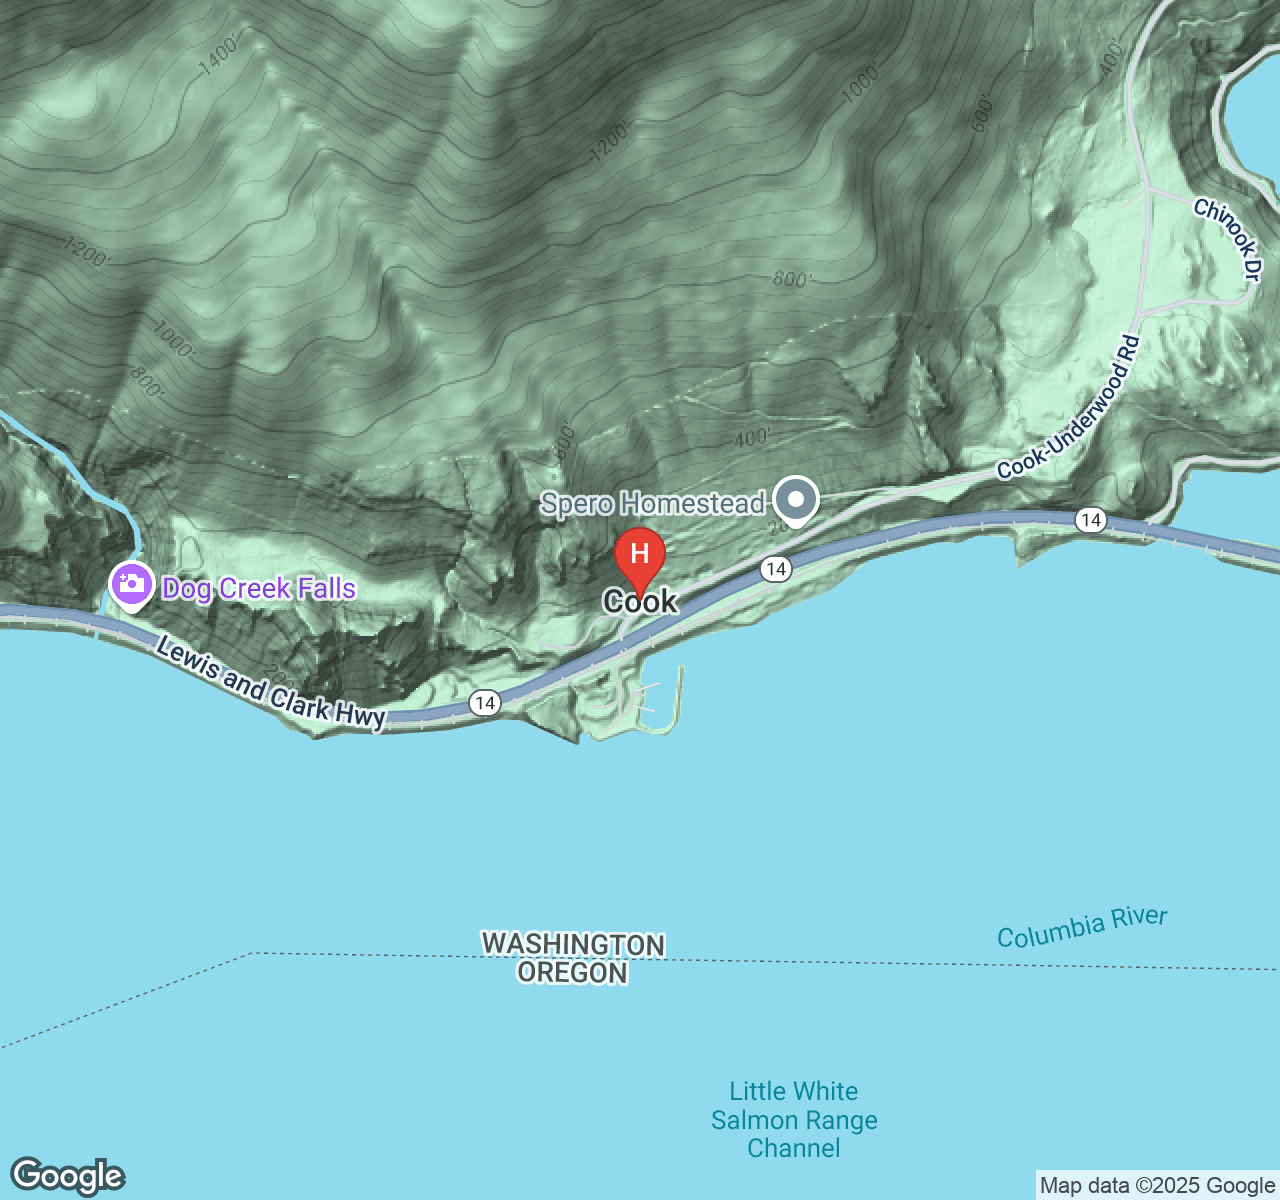
\includegraphics[keepaspectratio]{images/cascade_locks_or_walking_map.png}}

}

\caption{Cascade Locks Walking Vicinity Map}

\end{figure}%

\textbf{Glamping:} Under Canvas Columbia River \textbar{} Cascade Locks
area

\textbf{Within Walking Distance of Cascade Locks:} - Bridge of the Gods
- Iconic Columbia River bridge crossing - Thunder Island Brewing - Local
brewery with river views - Historic Locks and Dam - Engineering marvel
and salmon viewing - Marine Park - Riverside park with trails and river
access - Columbia River Trail - Scenic walking and biking path -
Historic town center with local dining and shops

\newpage

\subsection{Seattle, Washington Walking
Map}\label{seattle-washington-walking-map}

\textbf{The Fairmont Olympic Seattle \textbar{} August 12-14}

\begin{figure}[H]

{\centering \pandocbounded{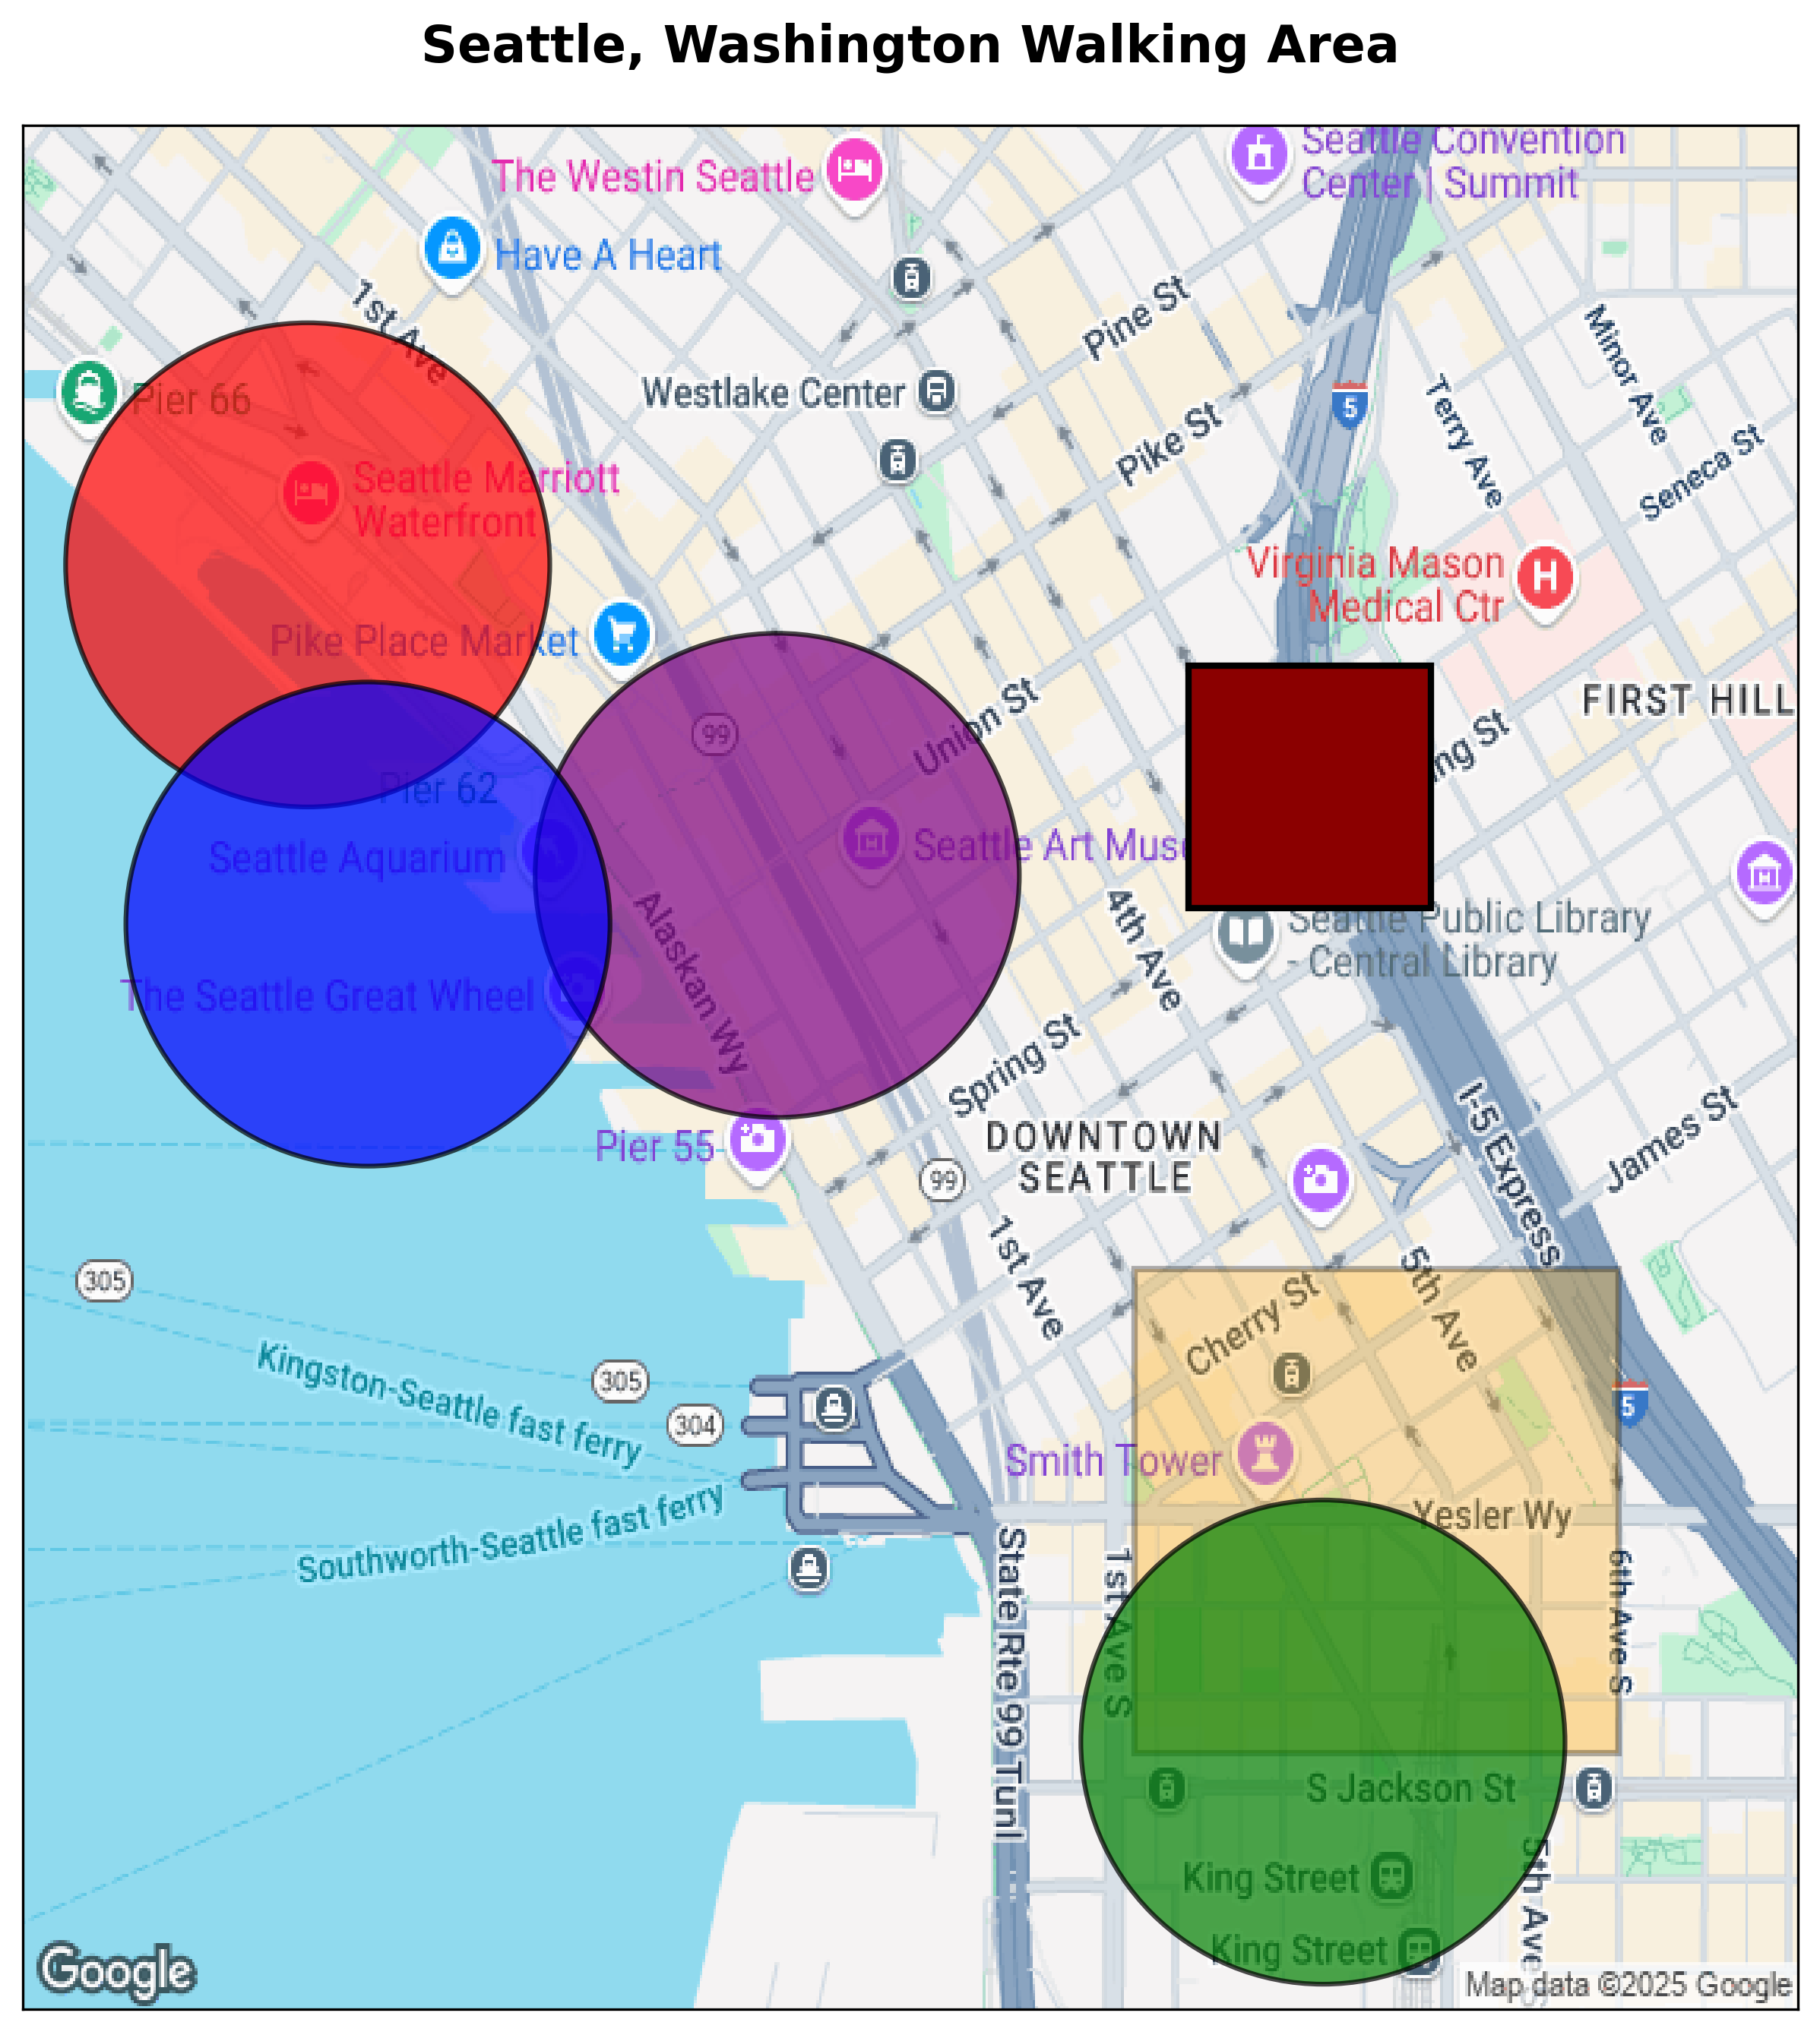
\includegraphics[keepaspectratio]{images/seattle_wa_walking_map.png}}

}

\caption{Seattle Walking Vicinity Map}

\end{figure}%

\textbf{Hotel:} The Fairmont Olympic Seattle \textbar{} 411 University
St \textbar{} (206) 621-1700

\textbf{Within Walking Distance:} - Pike Place Market - Iconic market
with fresh seafood and crafts - Seattle Art Museum - Premier Pacific
Northwest art collection - Pioneer Square - Historic district with
underground tours - Waterfront Park - Elliott Bay views and Olympic
Sculpture Park - Grand Central Bakery - Artisan sourdough and Pacific
Northwest breads - Benaroya Hall - Home of Seattle Symphony - Shopping
and dining throughout downtown core

\newpage

\section{Bozeman, Montana}\label{bozeman-montana}

\subsection{Day 1: August 3rd}\label{day-1-august-3rd}

\subsection{Bozeman, Montana}\label{bozeman-montana-1}

\textbf{August 3-4 \textbar{} Elevation: 4,820 ft}

\textbf{\href{images/bozeman_montana_recommendations_map.html}{View
Bozeman Recommendations Map}} - Interactive map showing all
recommendations around your hotel

\subsubsection{Walking Vicinity Map - Downtown
Bozeman}\label{walking-vicinity-map---downtown-bozeman}

\textbf{\href{images/bozeman_mt_walking_map.html}{View Satellite Walking
Map}} - Satellite view with 30-minute walking radius from your hotel

This detailed satellite map shows everything within walking distance of
Kimpton Armory Hotel, including Main Street Historic District, local
bakeries, breweries, parks, and cultural sites. The satellite imagery
with street overlays makes it easy to navigate on foot and see the
actual terrain and building layouts.

\subsubsection{Kimpton Armory Hotel
Bozeman}\label{kimpton-armory-hotel-bozeman}

Contact (406) 551-7700 \textbar{} kimptonarmoryhotel.com. Best Room:
Mountain View King (\$300-450/night). Amenities include boutique luxury,
fitness center, and pet-friendly accommodations.

\subsubsection{Activities}\label{activities}

Downtown exploration and local breweries, Montana State University
campus, and Museum of the Rockies.

\subsubsection{Glacial \& Geological Features - Montana
Leg}\label{glacial-geological-features---montana-leg}

\textbf{Glacial Lake Missoula Legacy}

The entire Montana route sits within the massive impact zone of Glacial
Lake Missoula floods. The Bozeman Area is positioned along the
floodplain of the Bozeman pass drainage, showing flood scour marks.
Geological evidence includes massive glacial erratics (out-of-place
boulders) visible throughout the valley and terrace formations from
catastrophic glacial outburst floods occurring approximately 15,000
years ago.

\textbf{Visible Glacial Features in Bozeman Area}

Glacial features include terminal and lateral moraines visible on
hillsides (especially north of town), large boulders scattered
throughout the valley floor, Gallatin Valley filled with glacial
sediment deposits, and step-like formations along the Gallatin River
from glacial dam-break floods.

\textbf{Specific Roadside Geology}

Road views include Interstate 90 approach through glacial-carved valley
with visible moraines on both sides, Highway 191 North with glacial
cirques visible in the Bridger Mountains, and Bridger Range showing
U-shaped glacial valleys and hanging valleys visible from town.

\subsubsection{Archaeological \& Paleontological
Sites}\label{archaeological-paleontological-sites}

\textbf{Museum of the Rockies (Bozeman)}

Located on Montana State University campus, the museum features the
world's largest collection of dinosaur fossils, including Maiasaura
(Montana's state fossil). Famous discoveries include the Egg Mountain
site with revolutionary dinosaur nesting ground discoveries and
interactive Maiasaura ``good mother reptile'' life-sized models and
replica skull exhibits. Hours: 9 AM - 5 PM daily. Admission: \$18
adults, \$13 seniors/students. Visit to see artifacts from nearby Egg
Mountain that changed how paleontologists understand dinosaur behavior.

\textbf{Pictograph Cave State Park (90 minutes from Bozeman)}

Located 23 miles southeast of Billings (side trip option), this National
Historic Landmark preserves 5,000+ years of human habitation. Features
include 100+ pictographs (rock paintings), 30,000+ artifacts excavated,
and the oldest art including 2,000-year-old turtle pictograph.
Archaeological impact includes the first definitive archaeological
report about Northwestern Plains (1951). Trail: 3/4 mile interpretive
loop with viewing platforms. Hours: 9 AM - 7 PM (summer), visitor center
10 AM - 5 PM. Admission: \$8 non-residents, \$4 walk-ins.

\subsubsection{Bakery Recommendations}\label{bakery-recommendations}

\textbf{Great Harvest Bread Co.}

Fresh-milled Montana wheat bread and daily artisan loaves. Featured:
Montana wheat sourdough, sunflower honey oat. Hours: Mon-Sat 6:30 AM - 6
PM.

\textbf{Wild Crumb Bakery \& Cafe}

European-style artisan breads with heritage sourdough starter. Featured:
Country sourdough, rye breads, ciabatta. Hours: Tues-Sat 7 AM - 3 PM.

\subsubsection{BBQ \& Smokehouse
Recommendations}\label{bbq-smokehouse-recommendations}

\textbf{Bar 3 BBQ \& Brewing} \textbar{} \emph{Belgrade (7 miles from
Bozeman)}

Must Try: Montana beef brisket, hickory-smoked pulled pork. Bonus: 10+
craft beers on tap. Hours: Daily 11 AM - 9 PM.

\textbf{Blue Smoke Barbeque} \textbar{} \emph{Bozeman}

Specialty: 100\% wood-smoked local meats. Featured: Smoked trout,
Montana beef brisket. Hours: Call ahead for availability.

\subsubsection{Specialty Dining}\label{specialty-dining}

\textbf{Blackbird Kitchen}

Wood-fired Argentine-style asado. Featured: Whole lamb shoulder,
cross-roasted meats. Hours: Daily 5 PM - 10 PM.

\textbf{Montana Wagyu} (by arrangement)

Custom whole lamb roasts with traditional Patagonian preparation. Farm
visits and asado cooking demonstrations available.

\subsection{Day 2: August 4th}\label{day-2-august-4th}

\textbf{Bozeman, Montana}

This first day establishes a base in Bozeman, Montana, requiring one
night accommodation to begin the Pacific Northwest adventure. Activities
encompass exploring the local area through hiking trails in the
surrounding mountains, visiting the farmers market for regional products
and artisan goods, and becoming acquainted with the Montana mountain
atmosphere that will characterize the journey ahead.

\textbf{Additional Archaeological Sites}

\textbf{Barton Gulch Archaeological Site (Historical Context)}

Located in Madison County, southwest Montana (Ruby River area), this
9,400-year-old Paleo-Indian site contains 37 archaeological features.
Discoveries include Clovis culture artifacts, hunting tools, and earth
ovens providing evidence of seasonal semi-nomadic hunter-gatherers.
Research was conducted by Montana State University's Dr.~Les Davis
(1987-1993). Note: Not open to public, but represents Montana's oldest
archaeological evidence.

\textbf{Montana Archaeological Significance}

Human presence in Montana dates back 13,000+ years. Artifacts include
stone tools, pottery fragments, and hunting implements from ancestors of
modern tribes including Crow, Blackfeet, and others. Evidence shows
inter-tribal trade networks spanning Great Basin to Northern Plains.

\newpage

\section{Missoula, Montana}\label{missoula-montana}

\subsection{Day 3: August 5th}\label{day-3-august-5th}

\textbf{Missoula, Montana}

\textbf{\href{images/missoula_montana_recommendations_map.html}{View
Missoula Recommendations Map}} - Interactive map centered on AC Hotel
Downtown

\subsubsection{Walking Vicinity Map - Downtown
Missoula}\label{walking-vicinity-map---downtown-missoula}

\textbf{\href{images/missoula_mt_walking_map.html}{View Satellite
Walking Map}} - Satellite view with 30-minute walking radius from your
hotel

This satellite map shows everything walkable from AC Hotel Missoula
Downtown, including the Clark Fork Riverfront Trail, University of
Montana campus, downtown historic district, local bakeries, and the
scenic Higgins Avenue Bridge. Perfect for exploring Missoula on foot
with clear satellite imagery and street overlays.

This day centers on Missoula, Montana, requiring one night accommodation
after a scenic 2-hour drive covering 142 miles from Bozeman. The AC
Hotel Missoula Downtown serves as downtown headquarters, reachable at
marriott.com/en-us/hotels/msoac-ac-hotel-missoula-downtown or (406)
541-8000, offering modern accommodations in the heart of the city.
Reservation requirements include booking two rooms, with accommodation
options featuring King Rooms providing one king bed, city views, and
corner room positioning for \$455 per night, or Two Queen Rooms offering
two queen beds accommodating four guests comfortably.

The optimal room request specifies ``high floor, west- or south-facing
corner room with panoramic city views, walk-in glass shower, no carpet''
to maximize the urban mountain experience. At \$455 per room per night,
total accommodation cost reaches \$910 for both rooms, though
availability remains limited requiring prompt reservation. Missoula
activities encompass walking the scenic Clark Fork Riverfront Trail,
exploring diverse local food establishments throughout downtown,
visiting the Rocky Mountain Elk Foundation for wildlife education, and
discovering the University of Montana campus with its historic
architecture and cultural offerings.

\subsubsection{\texorpdfstring{\textbf{The Revolutionary Geological
Discovery: Bretz's Two Flood
Stories}}{The Revolutionary Geological Discovery: Bretz's Two Flood Stories}}\label{the-revolutionary-geological-discovery-bretzs-two-flood-stories}

\textbf{This Missoula-Spokane route follows one of geology's most
controversial and revolutionary discoveries. Recent research reveals
that J Harlen Bretz actually proposed two different flood theories:}

\textbf{1. The Original ``Spokane Flood'' (1922-1927)}

Age: 150,000 to possibly 1 million years ago. Source: Canadian trench
systems (Rocky Mountain trench, Purcell trench). Mechanism: Subglacial
flow under the ``Spokane Ice Sheet''. Water Path: Down from Canadian
trenches, under ice, carving major channels. Evidence: Paleomagnetic
dating shows reversed polarity (older than 780,000 years). Impact:
Carved Grand Coulee, Moses Coulee, and major scabland channels.

\textbf{2. The Later ``Missoula Floods'' (1927 onward)}

Age: 19,000-15,000 years ago. Source: Glacial Lake Missoula ice dam
collapse (Joseph Pardee's contribution). Mechanism: Proglacial flooding
(out in front of ice sheet). Water Path: From Missoula lake through
already-carved channels. Evidence: Well-dated sediment layers,
rhythmites, current ripples. Impact: Added decorative sediment layers to
already-carved landscape.

\textbf{Evidence from the Astoria Fan (offshore Oregon)}

One-third of sediment from Missoula floods, two-thirds of sediment from
older Spokane floods. Implication: The older floods were twice as
massive as all Missoula floods combined.

\textbf{The Scientific Partnership}

J Harlen Bretz mapped the effects (scabland channels, flood evidence).
Joseph Thomas Pardee identified the cause (glacial Lake Missoula). In
1925, Pardee's crucial letter suggestion connected 500 cubic miles of
lake water to Bretz's flood evidence. Geographic Connection: Missoula
(Pardee's study area) to Spokane (Bretz's field site). Together: They
solved North America's greatest geological mystery.

\textbf{The Two Geological Giants}

Pardee (1871-1960): USGS geologist, worked western Montana, first to map
glacial Lake Missoula. Bretz (1882-1981): University of Chicago
professor, mapped channeled scablands, revolutionary catastrophist.
Professional Relationship: Cordial scientific correspondence led to
breakthrough understanding. Legacy: Their collaboration changed geology
from gradualism to accepting catastrophic events.

This route follows the path of both flood stories - the ancient Canadian
drainage system that carved the major landscape features over hundreds
of thousands of years, and the more recent Missoula flood deposits that
left the detailed sediment layers visible today.

\subsubsection{\texorpdfstring{\textbf{Specific Evidence Visible Along
This
Route:}}{Specific Evidence Visible Along This Route:}}\label{specific-evidence-visible-along-this-route}

\textbf{Large Current Ripples on Glacial Lake Missoula Floor}

Massive current ripples are visible across the Missoula valley floor,
appearing as wave-like patterns best observed from elevated viewpoints
around the city. These enormous ripples reach heights exceeding 20 feet
with spacing of more than 300 feet between crests, formed by the
catastrophic drainage events that repeatedly emptied glacial Lake
Missoula.

\textbf{Glacial Lake Missoula Shoreline Terraces}

Step-like formations visible on hillsides surrounding Missoula represent
ancient shorelines from multiple lake levels created by repeated dam
breaks and refilling cycles. Each horizontal terrace line marks a
consistent elevation where the lake surface remained stable, with each
terrace representing one complete cycle of lake formation, catastrophic
drainage, and refilling.

\textbf{Large Glacial Erratics}

Massive out-of-place boulders scattered throughout the route represent
Canadian Rockies granite transported far from their original geology.
These erratics, some reaching 40 feet in diameter, were carried by
icebergs floating in the flood waters and deposited on hillsides as the
icebergs melted and grounded during the massive drainage events.

\textbf{Paleomagnetic Evidence Sites}

Geological formations in the Morango area of eastern Washington contain
flood layers with reversed magnetic polarity, indicating they formed
more than 780,000 years ago during Earth's last magnetic field reversal.
This paleomagnetic evidence proves that multiple generations of
catastrophic floods occurred across vastly different geological time
periods, supporting the theory of both ancient Spokane floods and more
recent Missoula floods.

\textbf{Rhythmite Layers}

Road cuts along the route expose distinctive alternating layers of
coarse gravel and fine silt that record individual flood cycles. Each
rhythmite couplet represents one complete flood event, with coarse
material deposited during peak flow and fine sediments settling during
slack water periods. More than 40 separate flood events spanning 2,000
years are recorded in these sedimentary sequences.

\textbf{The Astoria Fan Connection:} All the eroded rock from these
floods had to go somewhere - it created a large underwater fan offshore
Oregon. Recent drilling reveals that 2/3 of this sediment pile comes
from the older Spokane floods, with only 1/3 from the well-known
Missoula floods.

\subsubsection{Archaeological \& Cultural
Sites}\label{archaeological-cultural-sites}

\textbf{University of Montana Archaeological Collections}

The University of Montana's Anthropology Department maintains
significant archaeological research collections focused on regional
studies and artifact preservation. Ongoing projects examine Northwestern
Plains prehistory while offering archaeological field school programs
for students. The department regularly displays current research
findings and welcomes inquiries about regional archaeological
discoveries.

\textbf{Historical \& Cultural Context}

The Missoula area represents traditional lands of the Salish, Kootenai,
and Pend d'Oreille peoples, with archaeological evidence documenting
continuous occupation spanning thousands of years. The river valley
location provided vital resources for indigenous communities, supporting
seasonal camps and permanent settlements. Modern tribal nations continue
active cultural preservation efforts, maintaining connections to
ancestral landscapes and traditional practices.

\textbf{Local Pottery \& Artisan Connections}

Downtown Missoula hosts numerous local artists and craft cooperatives
showcasing regional talent. Saturday farmers markets feature local
ceramics and indigenous-inspired crafts alongside agricultural products.
First Friday art walks highlight regional artists working in various
media, while the University of Montana ceramics program displays work by
Montana clay artists and student practitioners.

\subsubsection{Artisan Bakeries \& Fresh
Breads}\label{artisan-bakeries-fresh-breads}

\textbf{Le Petit Outre (Missoula)}

Located at 129 W Front St, Le Petit Outre specializes in French-style
pastries and European artisan breads using authentic French pastry
techniques. The bakery features pain de campagne, baguettes, croissants,
and seasonal tarts, offering genuine French breakfast pastries and
European breads in a Montana mountain setting. Open Tuesday through
Saturday, 7 AM to 3 PM, this establishment brings authentic French
baking traditions to the American West.

\textbf{Bernice's Bakery (Missoula)}

A local institution at 190 S 3rd St W, Bernice's Bakery has served
traditional American baking for decades, specializing in old-fashioned
donuts and classic breads. The bakery produces sourdough loaves, dinner
rolls, cinnamon rolls, and seasonal specialties using time-tested
recipes and methods. Open Monday through Saturday, 6 AM to 6 PM,
Bernice's represents traditional Montana bakery culture with comfort
food breads and classic American baking techniques.

\subsubsection{Incredible Smoked Meats, BBQ \&
Cheese}\label{incredible-smoked-meats-bbq-cheese}

\textbf{T-Rex BBQ (Three Forks - 30 minutes from Missoula)}

Located at 124 Main St in Three Forks, T-Rex BBQ specializes in what
locals call Montana's pride and joy brisket, described as ``some of the
best you'll ever have.'' The smokehouse features smoked trout, Montana
pork spareribs, and pineapple pork belly burnt ends, with unique
offerings including house-recipe jalapeño cheddar sausage and weekend
tri-tip roast. Operating Wednesday through Saturday from 11:30 AM to 7
PM (breakfast 6-9 AM), T-Rex represents authentic Montana barbecue using
dry rubs that are both gluten and sugar free.

\textbf{Riverhouse BBQ (Big Sky - 45 minutes from Missoula)}

Situated along the Gallatin River in Big Sky, Riverhouse BBQ combines
authentic Texas barbecue techniques with Montana mountain setting,
specializing in mesquite smoking methods. The restaurant features smoked
trout, Hill Country barbecue, and dry-rubbed meats served with riverside
dining and dramatic Spanish Peaks views. Open daily from 3 PM to 9 PM in
winter and 3 PM to 10 PM in summer, Riverhouse offers mesquite-smoked
meats in one of Montana's most stunning mountain river settings.

\subsubsection{Patagonian-Style Lamb \& Cross-Roasted
Meats}\label{patagonian-style-lamb-cross-roasted-meats}

\textbf{Plonk Wine Bar (Missoula)}

Located at 322 N Higgins Ave, Plonk Wine Bar specializes in
Argentine-inspired small plates and wine selections, featuring grilled
lamb prepared with chimichurri and paired with carefully selected wines.
The establishment offers extensive Argentine wine selections alongside
South American culinary influences, creating a wine country atmosphere
focused on lamb preparations and regional pairings. Open daily from 4 PM
to midnight, Plonk brings Argentine dining culture to Montana's wine bar
scene.

\textbf{Local Ranch Connections (Missoula Area)}

Bitterroot Valley ranches, located approximately 30 minutes south of
Missoula, offer custom lamb orders and ranch visit experiences featuring
grass-fed Montana lamb and ranch-to-table dining. These working ranches
provide authentic agricultural experiences including lamb preparation
demonstrations and farm-to-table meals showcasing regional livestock
production. Special arrangements can be made directly with local ranches
for visitors seeking authentic Montana ranch experiences and premium
locally-raised lamb.

\newpage

\section{Jerry Johnson Hot Springs}\label{jerry-johnson-hot-springs}

\subsection{Day 4: August 6th}\label{day-4-august-6th}

\textbf{Jerry Johnson Hot Springs}

\begin{figure}[H]

{\centering \pandocbounded{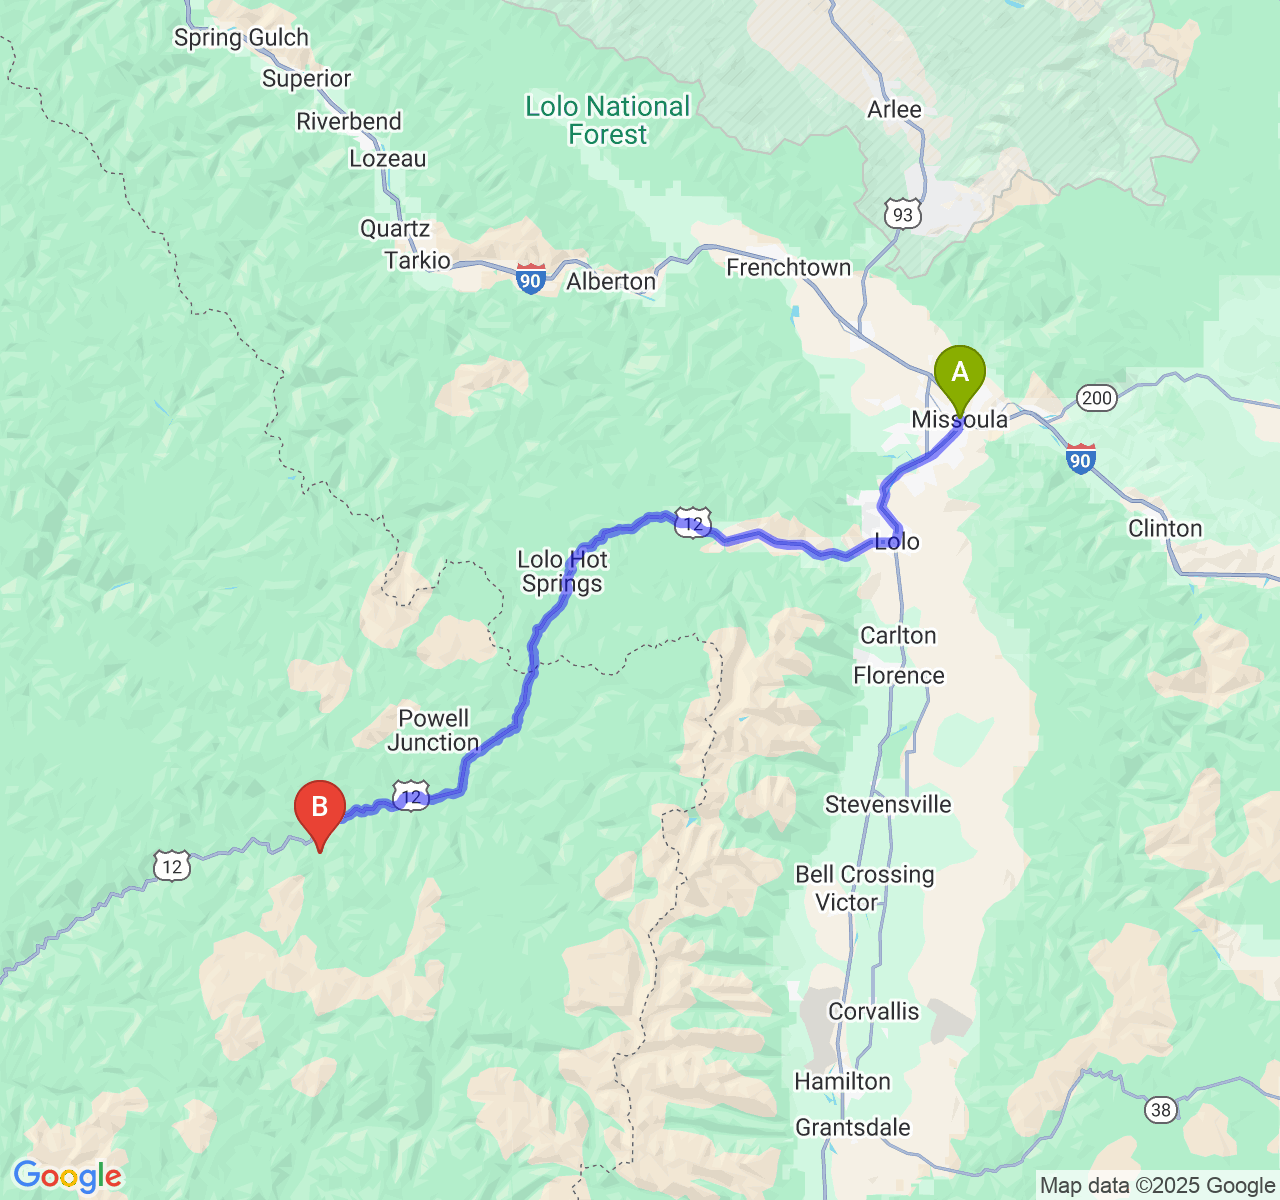
\includegraphics[keepaspectratio]{images/leg_2_Missoula_MT_to_Jerry_Johnson_Hot_Springs_ID.png}}

}

\caption{Route: Missoula to Jerry Johnson Hot Springs}

\end{figure}%

The route from Missoula to McCall follows Highway 12 (Scenic Byway) for
154 miles to Jerry Johnson Hot Springs, then continues 78 miles to
McCall. The special stop at Jerry Johnson Hot Springs requires a
one-mile hike from Mile Marker 152 on Highway 12 to reach three
different natural pool areas. The springs operate for day use only from
6 AM to 8 PM with no facilities available, requiring visitors to pack
everything in and out. From the hot springs, the route continues south
to McCall via scenic mountain roads through pristine wilderness areas.

\begin{figure}[H]

{\centering \pandocbounded{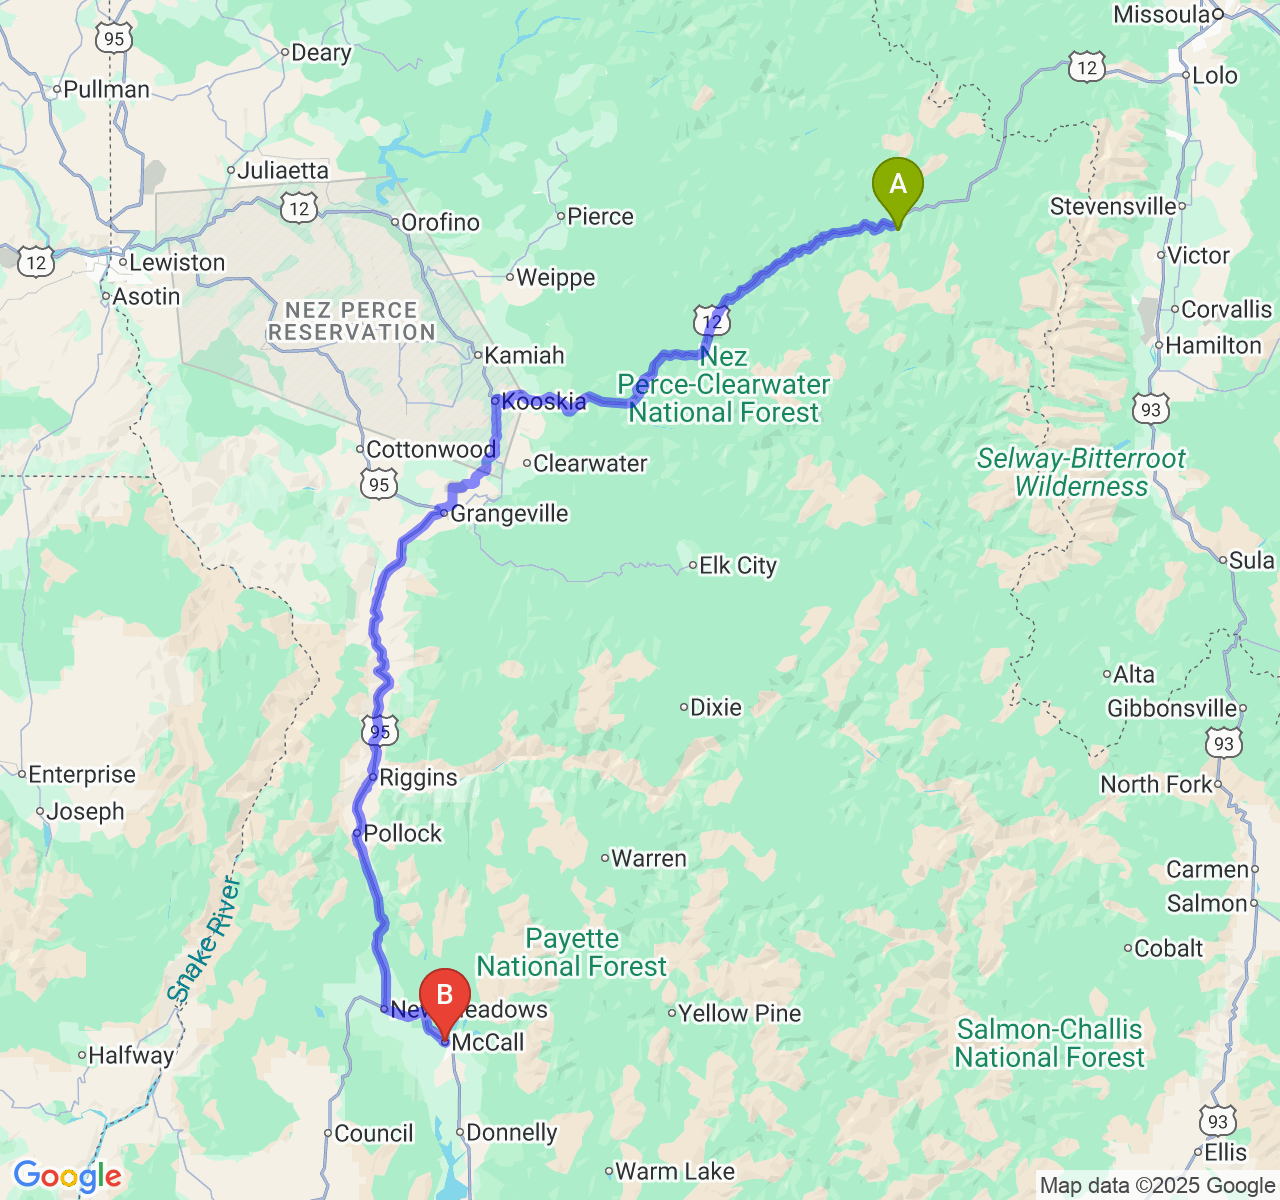
\includegraphics[keepaspectratio]{images/leg_3_Jerry_Johnson_Hot_Springs_ID_to_McCall_ID.png}}

}

\caption{Route: Jerry Johnson Hot Springs to McCall}

\end{figure}%

\subsubsection{Archaeological \& Cultural Sites Along Highway
12}\label{archaeological-cultural-sites-along-highway-12}

\textbf{Kelly Creek Archaeological Site (Historical Context)}

Located in Clearwater National Forest near the Montana-Idaho border, the
Kelly Creek Archaeological Site contains 12,000-year-old artifacts
representing some of Idaho's oldest evidence of human occupation.
University of Idaho excavations conducted between 2009-2012 uncovered
more than 11,000 artifacts including projectile points, spear tips, and
stone tools spanning from the Windust phase (earliest regional period)
through historic times. The site served as seasonal hunting and fishing
grounds for ancestors of the Nez Perce and Coeur d'Alene peoples, with
obsidian tools demonstrating extensive trade networks across the Pacific
Northwest. While not open to public visitation, this research site
represents significant regional archaeological importance in
understanding early human adaptation to mountain environments.

\textbf{Indigenous Cultural Landscape}

The Highway 12 corridor passes through traditional Nez Perce and Coeur
d'Alene territory, where these peoples established seasonal camps and
conducted systematic resource gathering for thousands of years. Natural
hot springs held both spiritual and practical importance in indigenous
culture, with traditional knowledge of thermal resources passed through
generations of tribal members. Modern tribal nations continue active
cultural preservation and education efforts, maintaining connections to
ancestral landscapes and traditional ecological knowledge.

\textbf{Nez Perce Cultural Heritage}

The Highway 12 corridor traverses ancestral Nez Perce lands, where
sophisticated resource management systems developed around understanding
seasonal resource cycles across diverse mountain and plateau
environments. Extensive trading relationships connected Nez Perce
communities across the Columbia Plateau, facilitating exchange of goods,
knowledge, and cultural practices. Active tribal efforts continue today
to maintain traditional practices and educate both tribal and non-tribal
communities about indigenous cultural heritage and ongoing connections
to traditional territories.

\subsubsection{Route Details: Highway 12 Scenic
Drive}\label{route-details-highway-12-scenic-drive}

Highway 12, also known as the Northwest Passage Scenic Byway, offers
spectacular mountain driving through the Lochsa Wild and Scenic River
corridor with sweeping views of the Selway-Bitterroot Wilderness. The
total driving time spans 3-4 hours including the hot springs stop,
following paved mountain roads with curves requiring careful driving.
This scenic route follows traditional indigenous travel corridors that
connected Columbia Plateau and Northern Plains cultures for thousands of
years.

\subsubsection{Glacial \& Geological Features - Highway 12
Route}\label{glacial-geological-features---highway-12-route}

\textbf{Lochsa River Valley Glacial Corridor}

The Highway 12 route follows the Lochsa River through a classic glacial
valley characterized by the perfect U-shaped profile carved by glacial
ice over multiple ice ages. This extremely deep canyon, reaching depths
of 4,000 feet, displays typical glacial erosion patterns with distinct
absence of V-shaped river cutting that would characterize stream-carved
valleys. The broad valley floor and steep sides represent the hallmark
characteristics of glacial carving processes.

\textbf{Specific Glacial Features Along Highway 12}

At Powell Junction, glacial cirque basins become visible in surrounding
peaks, while the Lowell Area displays glacial outwash terraces and
moraines from multiple ice advances. The Lochsa River follows the
glacial valley floor with typical glacial meandering patterns, while the
Bitterroot Range exhibits glacial horns and arêtes visible on ridge tops
throughout the drive.

\textbf{Alpine Glacial Features}

Bowl-shaped depressions carved by glacial ice in high country form
glacial cirques, while hanging valleys represent tributary valleys
positioned higher than the main valley floor. Glacial moraines consist
of rock debris deposited by glacial ice movement, and glacial striations
preserve scratch marks on exposed bedrock surfaces created by glacial
movement carrying rock fragments.

\textbf{Hot Springs Geological Context}

Thermal activity in the region associates with deep crustal fractures
exposed and enhanced by glacial carving processes. Geothermal systems
became accessible through glacial erosion that removed overlying rock
layers, while water sources derive from snowmelt infiltrating through
glacial deposits and bedrock fractures to reach heated zones at depth.

\newpage

\section{McCall, Idaho}\label{mccall-idaho}

\subsection{Day 5-6: August 7th-8th}\label{day-5-6-august-7th-8th}

\textbf{Shore Lodge, McCall}

\textbf{\href{images/mccall_idaho_recommendations_map.html}{View McCall
Recommendations Map}} - Interactive map showing hot springs, dining, and
activities around Shore Lodge

\subsubsection{Walking Vicinity Map - McCall Town
Center}\label{walking-vicinity-map---mccall-town-center}

\textbf{\href{images/mccall_id_walking_map.html}{View Satellite Walking
Map}} - Satellite view with 30-minute walking radius from Shore Lodge

This satellite map shows the beautiful lakefront setting of Shore Lodge
and everything walkable in McCall, including Payette Lake Beach,
downtown shops and restaurants, Legacy Park, and the charming mountain
town atmosphere. The satellite imagery clearly shows the lake, forest,
and town layout for easy navigation.

Shore Lodge is a luxury lakefront resort located in McCall, Idaho, at
5,021 feet elevation on Payette Lake, offering two-night accommodations
with premium amenities and services. The resort can be reached at
shorelodge.com or (800) 657-6464, with recommended room requests for
lakefront suites featuring panoramic lake views, fireplaces, and private
balconies. Room options include Lakefront Suites with full lake views,
fireplaces, and balconies (\$500-700/night) or Premium Lake View rooms
with partial lake views and luxury amenities (\$400-600/night). Resort
amenities encompass spa services, fine dining, concierge assistance, and
direct lakefront access for recreational activities.

Resort dining centers on Narrows Steakhouse, serving wood-fired steaks,
smoked mountain game, and Idaho trout daily from 5:30 PM to 10 PM, while
the concierge can arrange custom dining experiences including
Patagonian-style lamb roasts and outdoor cooking demonstrations. Hot
spring day trips include Trail Creek Hot Springs with two rock pools
accessed via a 60-foot walk from parking, Burgdorf Hot Springs featuring
a historic resort with three pools (\$20/adult, reservations required),
and Gold Fork Hot Springs offering six tiered crystal pools
(\$10/adult). Special services encompass spa treatments, mountain
wellness programs, and lakefront activities including kayaking and
paddleboarding.

\subsubsection{Archaeological \& Cultural
Sites}\label{archaeological-cultural-sites-1}

\textbf{Wilson Butte Cave (South-central Idaho)}

Located in Twin Falls County approximately two hours south of McCall,
Wilson Butte Cave represents an important Paleo-Indian archaeological
site with significant research value. Excavations conducted in 1959-1960
and 1988-1989 revealed evidence of human occupation spanning thousands
of years, providing crucial insights into early hunter-gatherer
societies and habitation patterns. University studies continue to
analyze findings from this research site, which remains closed to public
tours but contributes substantially to understanding prehistoric human
adaptation in the region.

\textbf{Celebration Park (Day Trip Option - 3 hours south)}

Canyon County's Celebration Park, located near the Snake River, holds
the distinction of being Idaho's only archaeological park since its
establishment in 1989. The park features petroglyphs ranging from 100 to
10,000 years old preserved in basalt melon gravels, with activities
including atlatl demonstrations where visitors can try throwing ancient
hunting tools, interpretive trails with archaeological displays, and
guided tours of petroglyphs offered daily from 10 AM to 2 PM. The park
exists within Bonneville Flood geological formations, with a visitor
center providing educational displays on Paleolithic and Archaic
lifeways. Admission costs \$2 per vehicle with camping available,
offering visitors hands-on archaeological experiences with ancient
hunting demonstrations.

\textbf{Hells Canyon Archaeological Context (Eastern Idaho)}

Hells Canyon National Recreation Area contains significant
archaeological discoveries, including a 600-year-old Nez Perce textile
cache discovered in 2008 that contained cedar bark weaving materials and
basket components. The canyon preserves evidence of indigenous
occupation spanning more than 13,000 years, representing seasonal
hunting, fishing, and resource gathering areas used by successive
indigenous cultures. Modern tribal nations maintain active cultural
preservation efforts connected to these ancestral sites, ensuring
continuity of traditional knowledge and practices linked to this
remarkable landscape.

\subsubsection{Glacial \& Geological Features - McCall \& Payette
Lake}\label{glacial-geological-features---mccall-payette-lake}

\textbf{Payette Lake Glacial Formation}

Payette Lake formed through glacial damming and carving processes,
reaching depths of 314 feet typical of glacial lake formation. The
surrounding valley was carved by multiple glacial advances over
thousands of years, with terminal and lateral moraines visible around
the lake perimeter marking the extent of ice sheet movement and
deposition.

\textbf{McCall Area Glacial Features}

Brundage Mountain displays glacial cirques and moraines visible on
modern ski slopes, while Payette National Forest preserves extensive
glacial features throughout the high country. Multiple U-shaped glacial
valleys radiate from McCall, creating the characteristic alpine
topography, with numerous high-country lakes formed by glacial carving
processes scattered throughout the mountainous terrain.

\textbf{Payette Mountains Glacial Legacy}

Bowl-shaped basins carved by glacial ice in high peaks form distinctive
glacial cirques, while sharp peaks resulted from glacial carving
attacking mountains from multiple sides to create glacial horns. Sharp
ridges formed between glacial cirques create glacial arêtes, and smooth
bedrock surfaces throughout the region preserve evidence of glacial
grinding and polishing during ice sheet movement.

\textbf{Hot Springs Geological Context - McCall Area}

Multiple hot springs systems around the McCall area emerge from deep
geological fractures, with geothermal activity enhanced by glacial
carving that exposed previously buried geothermal systems. These thermal
features produce mineral-rich waters from deep earth sources, creating
therapeutic soaking opportunities that combine geological processes with
recreational activities.

\subsubsection{Artisan Bakeries \& Fresh
Breads}\label{artisan-bakeries-fresh-breads-1}

\textbf{Pancake House \& Christmas Shop (McCall)}

Located at 209 N 3rd St, the Pancake House \& Christmas Shop specializes
in fresh-baked goods and traditional breakfast breads, serving as a
local institution with decades of reputation in the McCall community.
The establishment features sourdough pancakes, cinnamon rolls, fresh
muffins, and daily bread made from scratch, offering hearty breakfast
breads and mountain comfort food. Open daily from 7 AM to 2 PM, this
traditional mountain bakery represents authentic local baking culture
with time-tested recipes and methods.

\textbf{Rupert's at Hotel McCall}

Situated at 1101 N 3rd St within Hotel McCall, Rupert's specializes in
artisan breads and European-style pastries prepared by a professional
pastry chef. The hotel bakery features fresh-baked bread, croissants,
and seasonal pastries, offering elegant breakfast pastries and artisan
bread in a luxury mountain setting. Operating daily from 7 AM to 11 AM
during breakfast service, Rupert's provides professional-quality baking
that combines European techniques with mountain hospitality.

\subsubsection{Incredible Smoked Meats, BBQ \&
Cheese}\label{incredible-smoked-meats-bbq-cheese-1}

\textbf{Shore Lodge Narrows Steakhouse}

Located at 501 W Lake St within Shore Lodge, the Narrows Steakhouse
specializes in wood-fired steaks and smoked mountain game, featuring
Idaho trout, smoked salmon, dry-aged steaks, and local game in an
exceptional lakefront dining setting with stunning mountain views. The
restaurant excels in fresh mountain fish and premium smoked meats,
operating daily from 5:30 PM to 10 PM and providing luxury mountain
dining with exceptional smoked fish preparations that showcase regional
ingredients and smoking traditions.

\textbf{Smoky Mountain Pizzeria \& Smokehouse (McCall)}

Located at 815 N 3rd St, Smoky Mountain Pizzeria \& Smokehouse
specializes in wood-fired pizza and house-smoked meats, featuring unique
offerings like smoked trout pizza, BBQ brisket, smoked salmon, and
mountain sausages prepared using wood-fired ovens and traditional
mountain smoking techniques. The establishment excels in smoked fish
specialties and mountain BBQ, operating daily from 11 AM to 10 PM and
representing local smoking traditions combined with authentic wood-fired
cooking methods that showcase regional ingredients and time-honored
techniques.

\subsubsection{Patagonian-Style Lamb \& Cross-Roasted
Meats}\label{patagonian-style-lamb-cross-roasted-meats-1}

\textbf{Shore Lodge Custom Dining}

Shore Lodge resort offers custom asado experiences and outdoor cooking
through their concierge services, specializing in whole lamb roasts,
open-fire cooking, and lakefront dining experiences with private chef
services and custom fire cooking arrangements. These special occasion
lamb experiences provide authentic asado dining in a luxury resort
setting, available through Shore Lodge concierge for private dining
arrangements that combine custom Argentine-style cooking with pristine
lakefront mountain ambiance.

\textbf{Local Ranch Connections (McCall Area)}

Meadows Valley ranches, located 45 minutes south of McCall, specialize
in grass-fed lamb and authentic ranch experiences, featuring mountain
lamb production, ranch tours, and working farm visits in high-altitude
grazing environments with pristine mountain settings. These
farm-to-table lamb operations provide authentic ranch experiences for
visitors seeking direct connections to Idaho mountain lamb production,
with special arrangements available through contact with local ranches
for immersive agricultural tourism experiences.

\subsubsection{Pottery \& Artisan Studios in McCall
Area}\label{pottery-artisan-studios-in-mccall-area}

\textbf{Local Pottery \& Artisan Connections}

The McCall area features numerous local ceramic artists and seasonal
craft fairs through McCall Arts \& Crafts, while Payette National Forest
preserves traditional pottery techniques and indigenous crafts
knowledge. Summer farmers markets showcase local ceramics alongside
agricultural products, and regional artist cooperatives support ceramic
artists working with clay and traditional materials, creating a vibrant
artisan community centered around traditional and contemporary pottery
practices.

\textbf{Indigenous-Inspired Arts}

Cultural education programs offer workshops on traditional pottery
techniques, while contemporary artists create modern interpretations
inspired by indigenous designs and traditional knowledge preservation
efforts. Collaborative projects between Native and non-Native artists
foster cultural exchange and artistic innovation, ensuring that
traditional pottery knowledge continues to influence contemporary
ceramic arts practice in the region.

\subsubsection{Artisan Workshop Access \& Creative
Ateliers}\label{artisan-workshop-access-creative-ateliers}

\textbf{Valley County Artist Community}

The Valley County artist community maintains working studios, pottery
studios, woodworking shops, and textile arts practices throughout the
area, with local artists' workshops and ateliers providing space for
ceramic artists working with regional clay and glazes, mountain
craftspeople working with local timber, and fiber artists and weavers
using regional materials in their creative practice.

\textbf{Informal Workshop Access}

Seasonal studio tours and informal visits provide artist open studio
experiences, while local artisans offer craft demonstrations showing
traditional techniques and apprentice opportunities for learning
traditional mountain crafts. Community workshops offer drop-in classes
and collaborative projects that welcome visitors to participate in
regional artistic traditions and learn from experienced local
craftspeople.

\textbf{Mountain Craft Traditions}

Traditional mountain crafts encompass timber arts working with local
pine, fir, and cedar, stone carving using regional granite and volcanic
stone, metalwork including blacksmithing and ironwork traditions, and
leather crafts using materials from local ranch operations, preserving
and continuing time-honored techniques adapted to mountain environments
and available materials.

\newpage

\section{Joseph, Oregon}\label{joseph-oregon}

\subsection{Day 7: August 9th}\label{day-7-august-9th}

\textbf{The Jennings Hotel, Joseph}

\textbf{\href{images/joseph_oregon_recommendations_map.html}{View Joseph
Recommendations Map}} - Interactive map showing Wallowa Lake, bronze
foundry, and mountain dining around Jennings Hotel

\subsubsection{Walking Vicinity Map - Joseph Town
Center}\label{walking-vicinity-map---joseph-town-center}

\textbf{\href{images/joseph_or_walking_map.html}{View Satellite Walking
Map}} - Satellite view with 30-minute walking radius from Jennings Hotel

This satellite map showcases Joseph's charming Main Street location and
everything within walking distance of Jennings Hotel, including Valley
Bronze foundry, arts center, local restaurants, and the historic western
town atmosphere. The satellite view clearly shows the mountain valley
setting and small-town layout.

The Jennings Hotel is a historic artist residency hotel located in
Joseph, Oregon, at 4,200 feet elevation in the Wallowa Valley, offering
one-night accommodations with unique artistic amenities and mountain
atmosphere. The hotel can be reached at jenningshotel.com or (541)
432-0230, with recommended room requests for historic rooms featuring
mountain views, original hardwood floors, and artist studio access. Room
types include Historic Suites with original 1920s charm and mountain
views (\$250-350/night) or Artist Studio Rooms with working studio space
and creative amenities (\$200-300/night). The hotel specializes in
artist residency programs with working studios on-site, offering
activities including Wallowa Lake visits, Chief Joseph Ranch tours, and
artist studio tours that showcase the active creative community.

\subsubsection{Archaeological \& Cultural
Sites}\label{archaeological-cultural-sites-2}

\textbf{Nez Perce National Historical Park (Wallowa Valley)}

Located in the Wallowa Valley of Oregon, the Nez Perce National
Historical Park preserves the ancestral homeland of the Nez Perce
people, documenting more than 13,000 years of continuous indigenous
habitation and serving as the birthplace and homeland of Chief Joseph
(Hin-mah-too-yah-lat-kekt). Cultural features include traditional
fishing sites on Wallowa Lake, seasonal hunting and gathering areas,
sacred sites and ceremonial grounds, and traditional root gathering
areas that supported sustainable indigenous lifeways for millennia. The
park offers interpretive trails and cultural education programs that
connect visitors to this rich cultural heritage, while the Nez Perce
tribe maintains active cultural preservation efforts that ensure
traditional knowledge and practices continue to inform park
interpretation and management.

\textbf{Wallowa Lake Archaeological Context}

Located at the end of Wallowa Valley, Wallowa Lake preserves a 10,000+
year archaeological record documenting continuous indigenous occupation
through discoveries of stone tools, fishing implements, and seasonal
camp sites. Evidence shows continuous seasonal use of the area as a
summer fishing and gathering destination, with ongoing university
studies examining seasonal habitation patterns and cultural adaptations
to alpine environments. Protected archaeological sites around the lake
ensure preservation of this significant cultural record for future
research and cultural education.

\textbf{Old Chief Joseph Gravesite}

The Old Chief Joseph Gravesite in Wallowa Valley marks the burial site
of Chief Joseph's father (Tuekakas), the leader who signed the 1855
Treaty establishing the Wallowa Reservation. This sacred site holds
profound cultural importance for the Nez Perce people, featuring a stone
marker commemorating his peaceful leadership and diplomatic efforts.
Respectful viewing with cultural interpretation provides visitors with
understanding of Nez Perce leadership and the complex history of treaty
negotiations in the Pacific Northwest.

\subsubsection{Glacial \& Geological Features - Wallowa
Mountains}\label{glacial-geological-features---wallowa-mountains}

\textbf{Wallowa Mountains Glacial Formation}

Extensive glacial carving created the dramatic alpine landscape of the
Wallowa Mountains through multiple U-shaped valleys carved by glacial
ice, bowl-shaped basins in high peaks from glacial carving, and terminal
and lateral moraines distributed throughout the valley system. This
glacial sculpturing over multiple ice ages produced the distinctive
``Alps of Oregon'' topography that characterizes the region today.

\textbf{Wallowa Lake Glacial Origin}

Wallowa Lake formed through glacial damming and carving processes,
reaching depths of 283 feet typical of glacial lake formation, with the
valley floor scoured by glacial ice movement and moraine deposits
forming a natural dam at the lake outlet. This glacial origin explains
the lake's exceptional depth and the characteristic steep-walled valley
that contains it.

\textbf{Eagle Cap Wilderness Glacial Features}

The Eagle Cap Wilderness preserves more than 50 high-country lakes
formed by glacial carving, along with sharp peaks formed by glacial
carving from multiple sides (glacial horns), sharp ridges formed between
glacial cirques (glacial arêtes), and smooth bedrock surfaces from
glacial grinding (glacial polish). These features represent some of the
most spectacular alpine glacial landscapes in the Pacific Northwest.

\textbf{Wallowa Mountains Geological Context}

The Wallowa Mountains consist primarily of granite and metamorphic
rocks, with glacial carving exposing diverse geological formations and
revealing gold and copper deposits through glacial activity. Structural
features including faults and fractures were enhanced by glacial
processes, creating the complex geological landscape that supports both
the dramatic scenery and the mineral wealth that attracted early
settlement to the region.

\subsubsection{Artisan Bakeries \& Fresh
Breads}\label{artisan-bakeries-fresh-breads-2}

\textbf{Embers Brewhouse \& Eatery (Joseph)}

Located at 204 N Main St, Embers Brewhouse \& Eatery specializes in
fresh-baked breads and artisan pizzas, featuring sourdough breads, pizza
crusts, fresh rolls, and daily pastries prepared using wood-fired ovens
and mountain grain breads. The establishment excels in artisan pizza
breads and mountain bakery goods, operating daily from 11 AM to 9 PM as
a local institution known for wood-fired bread baking that combines
traditional techniques with regional ingredients.

\textbf{Wallowa Lake Lodge Dining}

Situated at 60060 Wallowa Lake Hwy, Wallowa Lake Lodge Dining
specializes in fresh breakfast breads and mountain pastries, featuring
cinnamon rolls, fresh muffins, breakfast breads, and scones prepared in
a historic lodge setting with traditional mountain baking methods. The
lodge provides lakefront breakfast and mountain comfort food
experiences, operating daily from 7 AM to 2 PM for breakfast and lunch
service in an authentic historic mountain lodge atmosphere with
traditional baking practices.

\subsubsection{Incredible Smoked Meats, BBQ \&
Cheese}\label{incredible-smoked-meats-bbq-cheese-2}

\textbf{Lear's Main Street Grill (Joseph)}

Located at 111 W Main St, Lear's Main Street Grill specializes in smoked
meats and mountain BBQ, featuring smoked brisket, pulled pork, smoked
salmon, and mountain sausages prepared using local smoking traditions
and mountain game processing techniques. The restaurant excels in
authentic mountain BBQ and smoked specialties, operating daily from 11
AM to 9 PM as a local smokehouse that preserves traditional mountain BBQ
traditions and regional smoking methods.

\textbf{Wallowa Lake Lodge Smokehouse}

Situated at 60060 Wallowa Lake Hwy, Wallowa Lake Lodge Smokehouse
specializes in fresh-smoked fish and mountain game, featuring smoked
trout, salmon, elk, venison, and local cheeses prepared using lakefront
smoking and traditional techniques. The smokehouse excels in fresh
mountain fish and smoked game preparations, operating daily from 5 PM to
10 PM for dinner service as a traditional mountain smokehouse offering
lake-fresh fish in an authentic alpine setting.

\subsubsection{Patagonian-Style Lamb \& Cross-Roasted
Meats}\label{patagonian-style-lamb-cross-roasted-meats-2}

\textbf{Local Ranch Connections (Wallowa Valley)}

Wallowa Valley ranches offer grass-fed lamb and authentic ranch
experiences through arrangements coordinated via the Joseph visitor
center, featuring mountain lamb production, ranch tours, and working
farm visits in high-altitude grazing environments with pristine alpine
settings. These farm-to-table lamb operations provide authentic ranch
experiences showcasing Oregon mountain lamb in the spectacular valley
setting, with special arrangements available through direct contact with
local ranches for immersive agricultural tourism experiences.

\textbf{Wallowa Valley Festival of Arts (August Timing)}

The Wallowa Valley Festival of Arts takes place in downtown Joseph
during August, specializing in outdoor cooking demonstrations and
artisan food experiences featuring live cooking, local lamb, artisan
foods, and craft demonstrations. This unique artist community event
focuses on culinary arts integration, providing cultural experiences
with food artistry that showcase the intersection of creative and
culinary traditions. Visitors should check the August festival schedule
for special events that highlight the artist community's commitment to
food and craft integration.

\subsubsection{Pottery \& Artisan Studios in
Joseph}\label{pottery-artisan-studios-in-joseph}

\textbf{Valley Bronze of Oregon}

Located at 18 S Main St, Valley Bronze of Oregon specializes in bronze
casting and sculptural arts, featuring bronze sculptures, casting
demonstrations, and artist workshops in a working foundry with public
access. The facility excels in metal arts and sculptural techniques,
operating Monday through Saturday from 9 AM to 5 PM as an active foundry
that provides visitors with direct access to bronze casting expertise
and live demonstrations of traditional metalworking processes.

\textbf{Josephy Center for Arts \& Culture}

Situated at 403 N Main St, the Josephy Center for Arts \& Culture
specializes in local pottery and cultural arts, featuring ceramic
workshops, pottery classes, and cultural exhibits in a community arts
center with comprehensive educational programs. The center excels in
pottery learning and cultural engagement, operating Tuesday through
Saturday from 10 AM to 5 PM as a community arts hub that provides
pottery education and cultural programming that connects visitors to
regional artistic traditions.

\subsubsection{Artisan Workshop Access \& Creative
Ateliers}\label{artisan-workshop-access-creative-ateliers-1}

\textbf{The Jennings Hotel Artist Residency}

Located at 401 S Main St, The Jennings Hotel Artist Residency
specializes in artist studios and creative workshops, featuring working
studios, artist residencies, and creative workshops in a unique hotel
with integrated artist studios. The facility excels in creative
immersion and artist interaction, with hotel guests able to visit
studios and meet artists, creating a unique artist hotel experience with
an active creative community that combines accommodation with artistic
engagement.

\textbf{Wallowa Valley Artist Community}

The Wallowa Valley artist community maintains working studios, pottery
studios, woodworking shops, and textile arts practices throughout
Joseph, with local artists' workshops and ateliers providing space for
ceramic artists working with regional clay and glazes, mountain
craftspeople working with local timber, and fiber artists and weavers
using regional materials in their creative practices.

\textbf{Informal Workshop Access}

Seasonal studio tours and informal visits provide artist open studio
experiences, while local artisans offer craft demonstrations showing
traditional techniques and apprentice opportunities for learning
traditional mountain crafts. Community workshops offer drop-in classes
and collaborative projects that welcome visitors to participate in
regional artistic traditions and learn from experienced local
craftspeople.

\textbf{Mountain Craft Traditions}

Traditional mountain crafts encompass bronze work including foundry arts
and metal sculpture, timber arts working with local pine, fir, and
cedar, stone carving using regional granite and volcanic stone, and
leather crafts using materials from local ranch operations, preserving
and continuing time-honored techniques adapted to mountain environments
and available materials.

\subsection{Lostine, Oregon - Historic Ranching
Town}\label{lostine-oregon---historic-ranching-town}

\textbf{Distance from Joseph:} 8 miles north \textbar{} \textbf{Drive
Time:} 12 minutes \textbar{} \textbf{Elevation:} 3,640 ft

\textbf{\href{images/lostine_oregon_town_map.html}{View Interactive
Lostine Town Map}} - Detailed map showing all points of interest in this
charming mountain town

\textbf{Why Visit Lostine:}

Lostine represents the authentic spirit of Oregon's ranching heritage,
where working cattle ranches still define the valley's character and way
of life. This small mountain town serves as both a gateway to the Eagle
Cap Wilderness and a showcase of high-end design culture, creating a
unique blend of rugged frontier history and sophisticated contemporary
artistry. The town's main street preserves the atmosphere of a classic
Western ranching community while hosting one of the region's most
celebrated design destinations.

\textbf{Historic Character:}

The town embodies the legacy of 19th-century homesteading and cattle
ranching that shaped the entire Wallowa Valley. Original homestead
buildings and working ranches surround the town, preserving traditional
agricultural practices and architectural heritage that date back to the
1870s. The Lostine River flows through the center of town, providing the
water resources that made settlement possible and continue to support
both agricultural operations and recreational activities for visitors
seeking authentic mountain town experiences.

\textbf{M. Crow \& Co.~General Store - Design Destination}

This internationally renowned design store operates out of a restored
historic building on Main Street, showcasing handcrafted furniture and
home goods created by Tyler Hays and his design team. The store
represents a unique fusion of Pacific Northwest materials and
traditional craftsmanship techniques, producing furniture and objects
that have gained recognition in major design publications worldwide.
Visitors can explore working studios and observe artisans creating
contemporary pieces using traditional woodworking and metalworking
methods.

\textbf{Local Culture:}

Lostine Tavern serves as the social hub of the community, offering
hearty mountain fare in an authentic Western atmosphere where locals and
visitors gather to experience genuine small-town hospitality. The
historic Methodist Church anchors the community's cultural life,
representing the spiritual and architectural heritage that has sustained
mountain communities for generations. Community events and gatherings
preserve the collaborative spirit essential to ranching culture and
mountain living.

\textbf{Outdoor Access:}

The town provides direct access to Wallowa-Whitman National Forest
through Lostine Canyon Road, leading to trailheads for alpine lake
hiking and Eagle Cap Wilderness exploration. The Lostine River offers
excellent fishing opportunities and scenic relaxation areas where
visitors can experience the pristine mountain environment that defines
this region. Multiple hiking trails begin just minutes from town,
providing access to some of Oregon's most spectacular alpine scenery.

\textbf{Ranch Heritage:}

Working cattle ranches continue operating throughout the Lostine Valley,
maintaining traditional ranching practices and preserving the
agricultural landscape that has characterized this area for more than
150 years. Visitors can observe authentic ranching operations and
understand the relationship between land use, water management, and
sustainable agriculture that sustains both the local economy and the
valley's scenic character. Many ranches welcome respectful visitors
interested in learning about modern ranching and land stewardship
practices.

\textbf{Planning Your Visit:}

Lostine makes an excellent addition to any Joseph area itinerary,
offering a deeper understanding of regional culture and access to unique
shopping and dining experiences not available in larger towns. The short
drive from Joseph allows for easy exploration of both communities, with
Lostine providing a more intimate and authentic small-town atmosphere.
Plan to spend 2-3 hours exploring the town, visiting M. Crow \& Co., and
enjoying the peaceful mountain setting that embodies the best of
Oregon's ranching heritage.

\newpage

\section{Walla Walla, Washington}\label{walla-walla-washington}

\subsection{Day 8: August 10th}\label{day-8-august-10th}

\textbf{Eritage Resort, Walla Walla}

\textbf{\href{images/walla_walla_washington_recommendations_map.html}{View
Walla Walla Recommendations Map}} - Interactive map showing wineries,
historic sites, and wine country dining around Eritage Resort

\subsubsection{Walking Vicinity Map - Downtown Walla
Walla}\label{walking-vicinity-map---downtown-walla-walla}

\textbf{\href{images/walla_walla_wa_walking_map.html}{View Satellite
Walking Map}} - Satellite view with 30-minute walking radius from
Eritage Resort

This satellite map displays the beautiful wine country setting and
everything walkable from Eritage Resort, including downtown historic
district, wine tasting rooms, French bakeries, Pioneer Park, and the
Whitman College campus. The satellite imagery shows the valley landscape
and urban layout perfect for exploring on foot.

Eritage Resort is a luxury wine country resort located in Walla Walla,
Washington, at 1,000 feet elevation in the Walla Walla Valley, offering
one-night accommodations with premium wine country amenities and
services. The resort can be reached at eritage.com or (509) 394-4700,
with recommended room requests for lake view suites featuring private
balconies overlooking pristine lake and wine country, fireplaces, and
spa amenities. Room types include Lake View Balcony Suites with full
lake views, private balconies, and fireplaces (\$400-600/night), Lake
View Patio Suites with lake views, patio access, and luxury amenities
(\$350-500/night), or Mountain View Balcony Suites featuring Blue
Mountain views and vineyard vistas (\$300-450/night). The resort
specializes in wine country elegance with artisan food and craft focus,
offering activities including winery tours, artisan workshops, and
downtown historic district exploration.

\subsubsection{Archaeological \& Cultural
Sites}\label{archaeological-cultural-sites-3}

\textbf{Whitman Mission National Historic Site}

Located at 328 Whitman Mission Rd, the Whitman Mission National Historic
Site preserves the 1836 mission established by Dr.~Marcus and Narcissa
Whitman, documenting early pioneer settlement and cultural exchange as a
significant meeting point of indigenous and pioneer cultures. Ongoing
archaeological research includes excavations of mission buildings, while
the visitor experience features an interpretive center with cultural
exhibits and educational programs offering living history demonstrations
and cultural education for understanding early cultural interactions in
the Pacific Northwest.

\textbf{Fort Walla Walla Museum}

Situated at 755 Myra Rd, Fort Walla Walla Museum preserves the military
fort established in 1856, documenting 19th-century military and pioneer
history through cultural features including a pioneer village with
historic buildings, military artifacts and exhibits, archaeological
displays from regional excavations, and traditional crafts
demonstrations. The visitor experience encompasses historic buildings
and living history programs that provide educational value focused on
pioneer-era crafts and cultural preservation.

\textbf{Cayuse Indigenous Cultural Heritage}

The Walla Walla Valley region represents the ancestral homeland of the
Cayuse people, preserving more than 10,000 years of continuous
indigenous habitation through cultural features including traditional
fishing sites on the Walla Walla River, seasonal hunting and gathering
areas, sacred sites and ceremonial grounds, and traditional root
gathering areas for camas and bitterroot. Modern connections include
active cultural preservation by the Confederated Tribes of Umatilla,
with visitor education programs offering cultural interpretation and
tribal connections that maintain living relationships to ancestral
landscapes.

\subsubsection{Glacial \& Geological Features - Walla Walla
Valley}\label{glacial-geological-features---walla-walla-valley}

\textbf{Walla Walla Valley Glacial Formation}

The Walla Walla Valley formed through Missoula Floods that deposited
rich sediments throughout the valley, creating deep alluvial deposits
from glacial lake draining that formed exceptional wine-growing soils
and carved the current valley configuration through repeated glacial
flooding events.

\textbf{Blue Mountains Glacial Features}

The Blue Mountains preserve bowl-shaped basins in high peaks from
glacial carving (glacial cirques), U-shaped valleys carved by glacial
ice movement, terminal and lateral moraines throughout the region, and
high-country lakes formed by glacial carving processes.

\textbf{Walla Walla River Glacial Context}

Glacial flooding carved the Walla Walla River channel, creating
step-like terraces from glacial lake levels, alluvial fans from glacial
sediment deposits from mountain runoff, and excellent groundwater
storage systems within glacial deposits.

\textbf{Wine Country Geological Context}

The wine country rests on Columbia River basalt bedrock underlying the
valley, with rich glacial deposits perfect for viticulture, drainage
patterns created by glacial shaping that provide excellent vineyard
drainage, and a glacial valley configuration that creates the unique
wine terroir of the region.

\subsubsection{Artisan Bakeries \& Fresh
Breads}\label{artisan-bakeries-fresh-breads-3}

\textbf{Colville Street Patisserie}

Located at 1425 Plaza Way, Colville Street Patisserie specializes in
French pastries and artisan breads, featuring croissants, sourdough,
baguettes, and seasonal pastries prepared by a European-trained pastry
chef using traditional techniques. The patisserie excels in authentic
French breads and elegant pastries, operating Tuesday through Saturday
from 7 AM to 3 PM and providing professional French baking in a wine
country setting.

\textbf{Bright's Candies \& Bakery}

Situated at 226 E Main St, Bright's Candies \& Bakery specializes in
traditional breads and sweet treats, featuring fresh daily bread, dinner
rolls, sweet breads, and cookies produced by a family bakery with
decades of tradition. The bakery excels in classic American breads and
hometown baking, operating Monday through Saturday from 8 AM to 6 PM as
a historic bakery that maintains traditional recipes and community
connections.

\textbf{Walla Walla Bread Company}

Located at 1717 E Isaacs Ave, Walla Walla Bread Company specializes in
artisan sourdough and heritage grains, featuring natural sourdough,
whole grain breads, and ancient grains produced through natural
fermentation and local grain sourcing. The bakery excels in artisan
sourdough culture and heritage breads, operating Monday through Friday
from 7 AM to 5 PM and Saturday from 8 AM to 4 PM as an artisan bakery
committed to traditional sourdough methods.

\subsubsection{Incredible Smoked Meats, BBQ \&
Cheese}\label{incredible-smoked-meats-bbq-cheese-3}

\textbf{Smoke \& Mirrors}

Located at 1555 E Isaacs Ave, Smoke \& Mirrors specializes in artisan
smoked meats and craft BBQ, featuring smoked brisket, pulled pork,
smoked salmon, and artisan sausages prepared using wine country smoking
techniques with local wine pairings. The restaurant excels in gourmet
BBQ and wine country dining, operating Wednesday through Sunday from 11
AM to 8 PM and providing elevated BBQ with wine country sophistication
that combines traditional smoking methods with regional culinary
refinement.

\textbf{Walla Walla Cheese Company}

With multiple locations throughout the Walla Walla Valley, Walla Walla
Cheese Company specializes in artisan cheeses and local dairy products,
featuring farmstead cheeses, aged cheeses, fresh cheeses, and wine
pairings produced by local dairy farms using traditional cheesemaking
methods. The company excels in wine and cheese pairings and local dairy
tradition, with hours varying by location and representing local
cheesemaking with a wine country focus that showcases regional dairy
heritage.

\textbf{Jacoby's Storehouse}

Situated at 624 2nd Ave, Jacoby's Storehouse specializes in smoked fish
and gourmet foods, featuring smoked salmon, smoked trout, artisan meats,
and local cheeses prepared in a historic building using traditional
smoking methods. The storehouse excels in Pacific Northwest smoking and
gourmet selections, operating Monday through Saturday from 10 AM to 6 PM
as a historic smokehouse that preserves regional specialties and
traditional food preservation techniques.

\subsubsection{Patagonian-Style Lamb \& Cross-Roasted
Meats}\label{patagonian-style-lamb-cross-roasted-meats-3}

\textbf{Saffron Mediterranean Kitchen}

Located at 125 W Alder St, Saffron Mediterranean Kitchen specializes in
Mediterranean grilling and lamb specialties, featuring grilled lamb,
Mediterranean spices, and fire-roasted vegetables prepared using
Mediterranean techniques with local ingredients. The restaurant excels
in lamb specialties and fire-grilled cuisine, operating Tuesday through
Saturday from 5 PM to 9 PM and providing Mediterranean lamb preparation
with local sourcing that honors traditional Mediterranean cooking
methods.

\textbf{Local Ranch Connections (Walla Walla Valley)}

Located throughout the Walla Walla Valley (contact visitor center for
locations), local ranches specialize in grass-fed lamb and ranch
experiences, featuring valley lamb, ranch tours, and working farm visits
that showcase wine country grazing in a pristine valley environment. The
ranches excel in farm-to-table lamb and authentic ranch experiences,
requiring contact with local ranches for special arrangements and
offering Washington valley lamb in a wine country setting that
demonstrates sustainable agriculture.

\textbf{Walla Walla Farmers Market (Saturday)}

Situated at 4th Ave \& Main St, the Walla Walla Farmers Market
specializes in local lamb and artisan foods, featuring fresh lamb, local
ranchers, artisan foods, and craft demonstrations that provide direct
access from ranchers with community connections. The market excels in
meeting local producers and providing fresh lamb, operating Saturdays
from 9 AM to 1 PM seasonally as a community market with direct ranch
connections that strengthen local food systems.

\subsubsection{Pottery \& Artisan Studios in Walla
Walla}\label{pottery-artisan-studios-in-walla-walla}

\textbf{Downtown Walla Walla Art Galleries}

Located at multiple locations on Main St, the downtown art galleries
specialize in local pottery and regional arts, featuring ceramic arts,
pottery classes, and gallery exhibits that showcase wine country arts
with multiple gallery spaces. The galleries excel in regional pottery
and art gallery tours, with hours varying by gallery and representing a
concentrated art district with multiple pottery studios that celebrate
regional artistic traditions.

\textbf{Walla Walla Community College Fine Arts}

Located at 500 Tausick Way, Walla Walla Community College Fine Arts
specializes in pottery education and ceramic arts, featuring pottery
classes, ceramic workshops, and student exhibitions that provide
college-level instruction with community access. The program excels in
pottery learning and ceramic education, with hours varying by program
and offering educational pottery with community access that bridges
academic and community artistic engagement.

\subsubsection{Artisan Workshop Access \& Creative
Ateliers}\label{artisan-workshop-access-creative-ateliers-2}

\textbf{Walla Walla Artist Studio Community}

The artist studio community encompasses local artists' workshops and
ateliers throughout downtown, pottery studios where ceramic artists work
with regional clay and glazes, woodworking shops where craftspeople work
with local timber, and textile arts featuring fiber artists and weavers
using regional materials that create a vibrant creative ecosystem in the
wine country setting.

\textbf{First Friday Art Walk}

Located throughout downtown Walla Walla, the First Friday Art Walk
specializes in monthly art walks with open studios, featuring artist
studios, gallery openings, and craft demonstrations that create a
community event with artist interaction. The event excels in meeting
local artists and studio visits, occurring the first Friday of each
month from 5 PM to 8 PM as an active art community with monthly
celebrations that strengthen cultural connections.

\textbf{Informal Workshop Access}

The informal workshop system includes artist open studios with seasonal
studio tours and informal visits, craft demonstrations where local
artisans demonstrate traditional techniques, apprentice opportunities
for learning traditional wine country crafts, and community workshops
offering drop-in classes and collaborative projects that foster artistic
learning and community engagement.

\textbf{Wine Country Craft Traditions}

The wine country craft traditions encompass cooperage focused on
barrel-making and wood arts, metalwork including vineyard metalwork and
artistic ironwork, stone carving using regional basalt and stone, and
leather crafts working with local ranch leather and hides that preserve
traditional skills while serving modern wine country needs.

\newpage

\section{Columbia River Gorge}\label{columbia-river-gorge}

\subsection{Day 9: August 11th}\label{day-9-august-11th}

\textbf{Under Canvas Columbia River Gorge}

\textbf{\href{images/columbia_river_gorge_recommendations_map.html}{View
Columbia River Gorge Recommendations Map}} - Interactive map showing
waterfalls, breweries, and lodges around Under Canvas glamping

\subsubsection{Walking Vicinity Map - Cascade
Locks}\label{walking-vicinity-map---cascade-locks}

\textbf{\href{images/cascade_locks_or_walking_map.html}{View Satellite
Walking Map}} - Satellite view of Cascade Locks town

This satellite map shows the dramatic Columbia River Gorge setting and
everything walkable in Cascade Locks, including the iconic Bridge of the
Gods, historic locks and dam, Thunder Island Brewing, and the riverside
marine park. The satellite imagery clearly shows the river, cliffs, and
historic infrastructure of this unique gorge town.

Located in Cascade Locks, Oregon, Under Canvas provides one night of
luxury glamping resort accommodation at 200 ft elevation in the Columbia
River Gorge (website: undercanvas.com/camps/columbia-river-gorge, phone:
(888) 496-1148). The best tent request would be a deluxe safari tent
with gorge views, private bathroom, and king bed, with tent types
including Safari Deluxe featuring gorge views, private bathroom, and
king bed (\$300-500/night), and Stargazer tents with transparent roof
panels and luxury amenities (\$400-600/night). The resort specializes in
glamping with dramatic gorge views and outdoor adventure, offering
activities including waterfall tours, hiking, Bridge of the Gods, and
wind sports that showcase the magnificent Columbia River Gorge
landscape.

\subsubsection{Archaeological \& Cultural
Sites}\label{archaeological-cultural-sites-4}

\textbf{Petroglyph Beach \& Tsagaglalal (She Who Watches)}

Located at Columbia Hills State Park, Washington, this 10,000+ year
archaeological site preserves ancient petroglyphs with evidence of
continuous indigenous habitation, featuring the famous Tsagaglalal -
``She Who Watches'' - iconic rock art. The cultural features include
ancient petroglyphs and pictographs, traditional fishing sites, seasonal
gathering areas, and sacred ceremonial locations, with visitor
experiences featuring guided tours of petroglyphs (reservations
required) and active cultural preservation by local tribes for viewing
some of the oldest rock art in North America.

\textbf{Cascade Locks Historic District}

Located in Cascade Locks, Oregon, this historic district preserves the
1896 locks and dam system on the Columbia River, representing an
engineering marvel of 19th-century transportation that transformed river
transportation and salmon runs. Ongoing archaeological research studies
pre-dam cultural sites, while the visitor experience includes an
interpretive center with locks history and educational programs
featuring engineering and cultural history demonstrations for
understanding human impact on river systems.

\textbf{Bonneville Dam Cultural Heritage}

Located between Bonneville, Oregon and Washington, this 1937 dam
construction represents New Deal era engineering and cultural change,
featuring cultural elements including fish ladder and salmon viewing,
visitor center with cultural exhibits, archaeological displays from dam
construction, and traditional fishing site interpretations. The visitor
experience focuses on fish viewing and cultural education, providing
educational value about dam impact on indigenous fishing rights and the
transformation of traditional river use patterns.

\subsubsection{Glacial \& Geological Features - Columbia River
Gorge}\label{glacial-geological-features---columbia-river-gorge}

\textbf{Columbia River Gorge Glacial Formation}

The Columbia River Gorge formed through catastrophic Missoula Floods
that carved the gorge through glacial lake outburst floods, massive ice
dams and flooding that carved canyon walls, glacial sediments deposited
throughout the gorge, and geological processes occurring 15,000-13,000
years ago during the last ice age.

\textbf{Waterfall Glacial Context}

The waterfall formations reflect glacial processes including Multnomah
Falls as a 620-foot waterfall enhanced by glacial carving, Latourell
Falls where glacial carving exposed Columbia River basalt, Bridal Veil
Falls created by glacial valley carving, and Wahkeena Falls where
glacial processes enhanced water flow patterns.

\textbf{Crown Point \& Vista House Geological Context}

Crown Point and Vista House showcase glacial carving that created
dramatic cliffs and viewpoints, Columbia River basalt formations exposed
by glacial scouring, glacial erratics as boulder deposits from glacial
transport, and valley formation where glacial processes carved the
current gorge configuration.

\textbf{Wind Patterns \& Glacial Legacy}

The wind patterns reflect glacial legacy through gorge winds created by
glacial carving that produces a wind tunnel effect, windsurfing
conditions where glacial valley shape creates consistent winds, weather
patterns influenced by glacial geography affecting regional climate, and
microclimates created by glacial carving that established unique
ecological zones.

\subsubsection{Artisan Bakeries \& Fresh
Breads}\label{artisan-bakeries-fresh-breads-4}

\textbf{Cascade Locks Ale House \& Restaurant}

Located at 599 WaNaPa St, Cascade Locks Ale House \& Restaurant
specializes in fresh-baked breads and pub fare, featuring artisan rolls,
pizza crusts, fresh bread, and seasonal pastries with gorge views and
outdoor dining. The restaurant excels in casual dining and fresh baked
goods, operating daily from 11 AM to 9 PM and providing a gorge setting
with fresh daily baking that combines scenic beauty with artisan bread
production.

\textbf{Stevenson, WA Bakery Options (15 minutes north)}

Located in Stevenson, Washington, these bakery options specialize in
small-town bakeries and fresh goods, featuring daily bread, pastries,
and coffee accompaniments from community bakeries with local character.
The bakeries excel in authentic small-town and fresh baking, with hours
varying by location and representing local community with traditional
baking that preserves neighborhood bakery traditions.

\textbf{Hood River Bakery Connections (20 minutes east)}

Located in Hood River, Oregon, the bakery connections specialize in
artisan breads and gorge specialties, featuring sourdough, whole grain
breads, and seasonal specialties from a gorge location with mountain
views. The bakeries excel in mountain town atmosphere and artisan
quality, with hours varying by location and representing gorge town with
quality bakeries that showcase regional baking excellence.

\subsubsection{Incredible Smoked Meats, BBQ \&
Cheese}\label{incredible-smoked-meats-bbq-cheese-4}

\textbf{Thunder Island Brewing}

Located at 515 WaNaPa St, Thunder Island Brewing specializes in smoked
meats and craft beer, featuring smoked brisket, pulled pork, smoked
salmon, and local cheeses in a gorge setting with outdoor smoking. The
brewery excels in BBQ and beer with river views, operating daily from 11
AM to 10 PM as a gorge brewery with quality smoked meats that combines
craft brewing with traditional smoking techniques.

\textbf{Bonneville Hot Springs Resort Dining}

Located at 1252 E Cascade Dr, North Bonneville, Bonneville Hot Springs
Resort Dining specializes in smoked salmon and Pacific Northwest
cuisine, featuring cedar plank salmon, smoked trout, local game, and
artisan cheeses at a hot springs resort with gorge views. The resort
excels in elegant dining and smoked fish specialties, operating daily
from 5 PM to 9 PM as resort dining with gorge salmon tradition that
honors Pacific Northwest culinary heritage.

\textbf{Local Smokehouse Connections}

Located at various locations in the Columbia River Gorge, local
smokehouse connections specialize in traditional salmon smoking and
Native American techniques, featuring cedar plank salmon, alder-smoked
fish, and traditional methods that showcase indigenous smoking
traditions and river connections. The smokehouses excel in authentic
Northwest and traditional techniques, requiring contact with local
tribal cultural centers for demonstrations and representing traditional
smoking with cultural connections that preserve ancestral food
practices.

\subsubsection{Patagonian-Style Lamb \& Cross-Roasted
Meats}\label{patagonian-style-lamb-cross-roasted-meats-4}

\textbf{Skamania Lodge}

Located at 1131 SW Skamania Lodge Way, Stevenson, Skamania Lodge
specializes in fire-grilled meats and outdoor cooking, featuring grilled
lamb, fire-roasted vegetables, and outdoor dining in a lodge atmosphere
with gorge views. The lodge excels in special occasion dining and
fire-grilled cuisine, operating daily from 5 PM to 10 PM as a luxury
lodge with fire-grilled specialties that combines elegant dining with
dramatic gorge scenery.

\textbf{Local Ranch Connections (Gorge Area)}

Located at Columbia River Gorge ranches, local ranch connections
specialize in grass-fed lamb and ranch experiences, featuring gorge
lamb, ranch tours, and working farm visits that showcase gorge grazing
in a river valley environment. The ranches excel in farm-to-table lamb
and authentic ranch experiences, requiring contact with local ranches
for special arrangements and offering gorge lamb in a dramatic river
setting that demonstrates sustainable agriculture.

\textbf{Outdoor Cooking Demonstrations}

Located at various gorge locations, outdoor cooking demonstrations
specialize in open-fire cooking and outdoor techniques, featuring
fire-roasted lamb, outdoor cooking classes, and traditional methods in a
gorge setting with natural cooking opportunities. The demonstrations
excel in learning outdoor cooking and fire techniques, requiring contact
with local outdoor programs for demonstrations and representing gorge
setting with outdoor cooking traditions that preserve wilderness
culinary skills.

\subsubsection{Pottery \& Artisan Studios in Columbia River
Gorge}\label{pottery-artisan-studios-in-columbia-river-gorge}

\textbf{Stevenson, WA Artist Community}

Located in Stevenson, Washington, the artist community specializes in
local pottery and regional arts, featuring ceramic arts, pottery
classes, and gallery exhibits that showcase small-town arts with gorge
inspiration. The community excels in regional pottery and community
connections, with hours varying by artist and representing community
arts with gorge setting that captures the natural beauty of the Columbia
River Gorge.

\textbf{Hood River, OR Artist Studios (20 minutes east)}

Located in Hood River, Oregon, the artist studios specialize in mountain
pottery and artisan studios, featuring ceramic arts, pottery workshops,
and artist studios that showcase mountain town arts with gorge views.
The studios excel in mountain pottery and studio visits, with hours
varying by studio and representing mountain arts community with gorge
connections that blend alpine and river valley influences.

\textbf{Gorge Artists Open Studios}

Located at various locations throughout the Columbia River Gorge, gorge
artists open studios specialize in regional pottery and gorge-inspired
arts, featuring ceramic arts, pottery demonstrations, and artist visits
that showcase gorge setting with landscape inspiration. The studios
excel in regional arts and scenic inspiration, operating during seasonal
open studio events and representing gorge artists with natural
inspiration that transforms dramatic landscapes into artistic
expression.

\subsubsection{Artisan Workshop Access \& Creative
Ateliers}\label{artisan-workshop-access-creative-ateliers-3}

\textbf{Columbia River Gorge Artist Community}

The Columbia River Gorge Artist Community encompasses local artists'
workshops and ateliers throughout the gorge, pottery studios where
ceramic artists work with regional clay and glazes, woodworking shops
where craftspeople work with local timber, and textile arts featuring
fiber artists and weavers using regional materials that create a vibrant
creative ecosystem inspired by the dramatic gorge landscape.

\textbf{Gorge Outdoor Education Centers}

Located at various gorge locations, gorge outdoor education centers
specialize in outdoor skills and traditional crafts, featuring
wilderness skills, traditional crafts, and outdoor workshops that
provide gorge setting with outdoor education. The centers excel in
learning outdoor skills and traditional techniques, requiring contact
with local outdoor programs for workshop schedules and representing
gorge setting with outdoor craft traditions that preserve wilderness
skills within spectacular natural settings.

\textbf{Informal Workshop Access}

The informal workshop access includes artist open studios with seasonal
studio tours and informal visits, craft demonstrations where local
artisans demonstrate traditional techniques, apprentice opportunities
for learning traditional gorge crafts, and community workshops offering
drop-in classes and collaborative projects that foster artistic learning
and creative community engagement throughout the Columbia River Gorge.

\textbf{Gorge Craft Traditions}

The gorge craft traditions encompass stone carving using regional basalt
and Columbia River stone, woodworking with Douglas fir and local timber,
metalwork including blacksmithing and ironwork traditions, and fiber
arts working with regional wool and natural fibers that preserve
traditional skills while drawing inspiration from the unique materials
and landscapes of the Columbia River Gorge region.

\newpage

\section{Seattle, Washington}\label{seattle-washington}

\subsection{Day 10-12: August
12th-14th}\label{day-10-12-august-12th-14th}

\textbf{The Fairmont Olympic Seattle}

\textbf{\href{images/seattle_washington_recommendations_map.html}{View
Seattle Recommendations Map}} - Interactive map showing Pike Place
Market, neighborhoods, and restaurants around Fairmont Olympic

\subsubsection{Walking Vicinity Map - Downtown
Seattle}\label{walking-vicinity-map---downtown-seattle}

\textbf{\href{images/seattle_wa_walking_map.html}{View Satellite Walking
Map}} - Satellite view with 30-minute walking radius from Fairmont
Olympic

This satellite map reveals the urban setting and everything walkable
from The Fairmont Olympic Seattle, including Pike Place Market, Seattle
Art Museum, Pioneer Square, the waterfront, Olympic Sculpture Park, and
Benaroya Hall. The satellite imagery shows the city grid, Elliott Bay
waterfront, and downtown landmarks perfect for urban exploration on
foot.

Located in Seattle, Washington, The Fairmont Olympic Seattle provides
two nights of accommodation in a historic luxury hotel from 1924 at sea
level at Puget Sound (website: fairmont.com/seattle, phone: (206)
621-1700). The best room request would be a high floor Olympic Suite
with city views, luxury amenities, and historic charm, with room types
including Olympic Suite featuring city views, luxury amenities, and
historic details (\$400-600/night), and Deluxe City View rooms with high
floor, downtown views, and premium location (\$300-500/night). This
hotel represents historic elegance, iconic status, and the perfect
capstone to a luxury journey, offering activities including Pike Place
Market, Space Needle, ferry tours, and museums, specializing in urban
exploration with Pacific Northwest culture in a historic luxury setting.

\textbf{Twin Peaks Stop - North Bend (August 12th)}

Located in North Bend, Washington (30 minutes from Seattle), this famous
Twin Peaks filming location offers featured stops including Salish Lodge
\& Spa as The Great Northern Lodge from the series, Twede's Cafe as The
RR Diner where Agent Cooper enjoyed ``damn fine coffee,'' and North Bend
scenic overlooks featuring Snoqualmie Falls and Twin Peaks landscapes.
The location excels for TV series fans and Pacific Northwest scenery,
providing the opportunity to experience the iconic Twin Peaks atmosphere
and stunning Cascade mountain views that defined the series' atmospheric
setting.

\subsubsection{Archaeological \& Cultural
Sites}\label{archaeological-cultural-sites-5}

\textbf{Burke Museum of Natural History and Culture}

Located at the University of Washington, Seattle, the Burke Museum
serves as the premier Pacific Northwest archaeological and cultural
museum, preserving more than 10,000 years of Pacific Northwest
indigenous history through featured collections including Pacific
Northwest indigenous artifacts, archaeological discoveries from regional
excavations, traditional art and cultural objects, and contemporary
indigenous art. The visitor experience encompasses interactive exhibits
and cultural education programs, while educational programs offer
workshops on indigenous culture and archaeology, making this a
comprehensive destination for Pacific Northwest cultural heritage.

\textbf{Daybreak Star Cultural Center}

Located in Discovery Park, Seattle, the Daybreak Star Cultural Center
serves as an American Indian cultural center and gathering place
dedicated to contemporary indigenous cultural preservation, featuring
programs including traditional craft demonstrations, cultural education
workshops, art exhibitions and cultural events, and traditional food and
cooking demonstrations. The visitor experience focuses on cultural
programs and indigenous art, providing educational value about modern
indigenous culture and traditions as an active indigenous cultural
center with educational programs that maintain living cultural
connections.

\textbf{Pioneer Square Historic District}

Located in downtown Seattle, Pioneer Square Historic District preserves
the original Seattle settlement and archaeological site, documenting
1850s pioneer settlement and cultural development through cultural
features including historic buildings and architecture, underground
tours of original streets, archaeological displays from early
settlement, and pioneer-era artifacts and exhibits. The visitor
experience includes historic walking tours and underground exploration,
while educational programs focus on pioneer history and urban
archaeology that reveals the layers of Seattle's founding and
development.

\subsubsection{Glacial \& Geological Features - Seattle \& Puget
Sound}\label{glacial-geological-features---seattle-puget-sound}

\textbf{Puget Sound Glacial Formation}

Puget Sound formed through massive glacial ice sheet carving that
reached depths of 930 feet from glacial scouring, occurring
15,000-13,000 years ago during the last ice age and creating the current
sound geography through glacial retreat processes that shaped the
distinctive marine landscape of the Pacific Northwest.

\textbf{Seattle Hills Glacial Context}

Seattle's distinctive topography reflects glacial processes including
the seven hills formed by glacial deposits creating glacial drumlins,
the city built on extensive glacial sediments and deposits known as
glacial till, large boulders transported by glacial ice and deposited as
glacial erratics, and step-like formations from glacial lake levels
creating the glacial terraces that characterize the urban landscape.

\textbf{Mount Rainier Glacial Connection}

Mount Rainier's glacial system connects to regional glaciation through
Mount Rainier glaciers that fed the Puget Sound ice sheet, glacial
carving that created current mountain valleys, glacial meltwater that
carved current river systems, and glacial deposits visible throughout
the region as moraines that document the extent and retreat of the
massive ice sheets.

\textbf{Elliott Bay Glacial Context}

Elliott Bay formed through glacial ice movement that carved the bay
configuration, with bay depth resulting from glacial scouring and
carving processes, harbor sediments derived from glacial deposits, and
the current shoreline shaped by glacial processes that created the
distinctive marine environment surrounding Seattle.

\subsubsection{Artisan Bakeries \& Fresh
Breads}\label{artisan-bakeries-fresh-breads-5}

\textbf{Grand Central Bakery}

Located at multiple Seattle locations, Grand Central Bakery specializes
in artisan sourdough and European-style breads, featuring natural
sourdough, whole grain breads, and seasonal specialties produced using
traditional fermentation and local grain sourcing. The bakery excels in
artisan bread culture and fermentation expertise, operating daily from
6:30 AM to 6 PM as a Seattle institution with traditional bread making
that has defined the city's artisan baking standards for decades.

\textbf{Macrina Bakery}

Located at multiple Seattle locations, Macrina Bakery specializes in
artisan pastries and fresh breads, featuring croissants, sourdough,
seasonal pastries, and specialty breads created using European
techniques with Pacific Northwest ingredients. The bakery excels in
elegant pastries and artisan breads, operating daily from 7 AM to 7 PM
and representing Seattle bakery excellence with European tradition that
combines Old World techniques with regional ingredients.

\textbf{Tall Grass Bakery}

Located at 1579 15th Ave, Tall Grass Bakery specializes in organic
breads and heritage grains, featuring organic sourdough, ancient grains,
and whole grain breads produced with organic certification and
sustainable practices. The bakery excels in organic baking and
sustainable bread production, operating Wednesday through Sunday from 8
AM to 3 PM as an organic bakery with sustainable focus that demonstrates
environmental responsibility in artisan bread making.

\subsubsection{Incredible Smoked Meats, BBQ \&
Cheese}\label{incredible-smoked-meats-bbq-cheese-5}

\textbf{Pike Place Market - Pure Food Fish Market}

Located at Pike Place Market, Seattle, Pure Food Fish Market specializes
in fresh-smoked salmon and Pacific Northwest fish, featuring cedar plank
salmon, smoked salmon, dungeness crab, and local oysters prepared using
market tradition with fish throwing demonstrations. The market excels in
fresh Pacific fish and market experience, operating daily from 6:30 AM
to 6 PM as an iconic market with fresh smoked fish that represents the
quintessential Seattle seafood experience.

\textbf{Beecher's Handmade Cheese}

Located at Pike Place Market, Seattle, Beecher's Handmade Cheese
specializes in artisan cheeses and traditional cheesemaking, featuring
flagship cheddar, fresh curds, aged cheeses, and mac and cheese produced
through visible cheesemaking and daily production. The cheese company
excels in artisan cheese and traditional techniques, operating daily
from 9 AM to 7 PM and providing opportunities to watch cheesemaking and
taste fresh cheese in the heart of Seattle's most famous market.

\textbf{Westman's Bagel \& Coffee}

Located at 2954 4th Ave S, Westman's Bagel \& Coffee specializes in
smoked fish bagels and Pacific Northwest flavors, featuring smoked
salmon bagels, lox, cream cheese, and Pacific specialties that showcase
Pacific Northwest bagels with local fish. The establishment excels in
regional bagel culture and smoked fish, operating daily from 6 AM to 4
PM and representing local bagel tradition with Pacific Northwest fish
that creates a distinctive regional breakfast experience.

\subsubsection{Patagonian-Style Lamb \& Cross-Roasted
Meats}\label{patagonian-style-lamb-cross-roasted-meats-5}

\textbf{Asado (Ballard)}

Located at 2810 NW Market St, Asado specializes in Argentine grilling
and authentic asado, featuring grilled lamb, Argentine beef,
fire-roasted vegetables, and chimichurri prepared using authentic
Argentine techniques with Pacific Northwest ingredients. The restaurant
excels in authentic asado and Argentine lamb, operating daily from 5 PM
to 10 PM and providing authentic Argentine cuisine with Pacific
Northwest connections that honor traditional South American grilling
methods.

\textbf{Matt's in the Market}

Located at 94 Pike St, Matt's in the Market specializes in fire-grilled
meats and market-fresh ingredients, featuring grilled lamb, fire-roasted
vegetables, and market ingredients sourced from its Pike Place Market
location with fire-grilled cuisine. The restaurant excels in
market-to-table dining and fire-grilled specialties, operating daily
from 5 PM to 10 PM as a market restaurant with fire-grilled excellence
that showcases the best of Pike Place Market ingredients.

\textbf{Local Ranch Connections (Puget Sound Area)}

Located throughout the Puget Sound region, local ranch connections
specialize in grass-fed lamb and authentic ranch experiences, featuring
Sound region lamb, ranch tours, and working farm visits that showcase
coastal grazing in a Pacific Northwest environment. These ranches excel
in farm-to-table lamb and authentic ranch experiences, requiring contact
with local ranches for special arrangements and offering Pacific
Northwest lamb in a unique coastal setting that demonstrates sustainable
agriculture practices within the region's distinctive maritime climate.

\subsubsection{Pottery \& Artisan Studios in
Seattle}\label{pottery-artisan-studios-in-seattle}

\textbf{Georgetown Studios}

Located in Georgetown neighborhood, Seattle, Georgetown Studios
specializes in artist studios and pottery workshops, featuring ceramic
arts, pottery classes, and artist studios in an industrial arts district
with multiple studios. The studios excel in urban pottery and studio
visits, with hours varying by studio and representing a concentrated
arts district with pottery focus that transforms industrial spaces into
vibrant creative environments.

\textbf{Pottery Northwest}

Located at 226 1st Ave S, Pottery Northwest specializes in community
pottery and ceramic education, featuring pottery classes, ceramic
workshops, and community studios through a community organization with
educational focus. The organization excels in pottery learning and
community connection, with hours varying by program and providing
community pottery with educational programs that make ceramic arts
accessible to all skill levels.

\textbf{Vermillion Art Gallery \& Bar}

Located at 1508 11th Ave, Vermillion Art Gallery \& Bar specializes in
local pottery and artisan exhibitions, featuring ceramic arts, pottery
exhibitions, and artist receptions in a gallery and bar with local
pottery focus. The venue excels in local pottery and artist community,
operating daily from 4 PM to 2 AM and providing a social pottery scene
with local artists that combines art appreciation with social gathering.

\subsubsection{Artisan Workshop Access \& Creative
Ateliers}\label{artisan-workshop-access-creative-ateliers-4}

\textbf{Seattle Artist Studio Community:}

The Seattle Artist Studio Community encompasses local artists' workshops
and ateliers throughout Seattle, pottery studios where ceramic artists
work with regional clay and glazes, woodworking shops where craftspeople
work with Pacific Northwest timber, and textile arts featuring fiber
artists and weavers using regional materials that create a diverse urban
creative ecosystem reflecting the city's artistic innovation.

\textbf{First Thursday Art Walk}

Located in Pioneer Square, Seattle, the First Thursday Art Walk
specializes in monthly art walks with open studios, featuring artist
studios, gallery openings, and craft demonstrations that create a
monthly community event with artist interaction. The event excels in
meeting local artists and studio visits, occurring the first Thursday of
each month from 6 PM to 9 PM as an active arts community with monthly
celebrations that strengthen cultural connections throughout the
historic district. This monthly community event provides unique
opportunities for direct artist interaction through open studios, with
featured artist studios, gallery openings, and craft demonstrations that
represent an active arts community with monthly celebration that builds
lasting cultural connections.

\textbf{Fremont Arts District}

Located in Fremont neighborhood, Seattle, the Fremont Arts District
specializes in quirky arts and creative workshops, featuring artist
studios, creative workshops, and unusual arts in a bohemian arts
district with creative energy. The district excels in alternative arts
and creative exploration, with hours varying by studio and representing
a creative neighborhood with artistic diversity that celebrates
unconventional artistic expression and community creativity.

\textbf{Informal Workshop Access}

The informal workshop access includes artist open studios with seasonal
studio tours and informal visits, craft demonstrations where local
artisans demonstrate urban techniques, apprentice opportunities for
learning contemporary city crafts, and community workshops offering
drop-in classes and collaborative projects that foster artistic learning
and creative community engagement throughout Seattle's neighborhoods.

\textbf{Seattle Craft Traditions}

The Seattle craft traditions encompass woodworking with Douglas fir and
Pacific Northwest timber, metalwork including industrial and artistic
metalwork traditions, glassblowing representing Pacific Northwest glass
arts, and fiber arts working with regional wool and sustainable
materials that preserve traditional skills while embracing urban
innovation and environmental consciousness.

\newpage

\section{San Juan Islands Finale}\label{san-juan-islands-finale}

\subsection{Day 12: August 12th - Twin Peaks Tour \& Island
Arrival}\label{day-12-august-12th---twin-peaks-tour-island-arrival}

\textbf{Twin Peaks Filming Locations → Round House Suite, Rosario
Village}

\textbf{\href{https://orcast.org}{View San Juan Islands Orca Probability
Map}} - Real-time orca sighting probabilities and interactive heatmap

\subsubsection{Morning: Twin Peaks Filming Locations
Tour}\label{morning-twin-peaks-filming-locations-tour}

\textbf{Route:} Under Canvas White Salmon → Mount Rainier National Park
→ North Bend → Snoqualmie Falls → San Juan Islands

\paragraph{Mount Rainier National Park - Scenic Drive (11:00 AM - 3:45
PM)}\label{mount-rainier-national-park---scenic-drive-1100-am---345-pm}

\textbf{Route Details:} - \textbf{Distance:} 189 miles via Mount Rainier
National Park - \textbf{Drive Time:} 4 hours 43 minutes (scenic mountain
route) - \textbf{Departure:} 11:00 AM from Under Canvas White Salmon -
\textbf{Arrival North Bend:} 3:45 PM - \textbf{Route:} State Route 14 →
I-205 → State Route 12 → Mount Rainier National Park → State Route 410 →
North Bend

\textbf{Scenic Highlights:} - \textbf{Mount Rainier Views:} Spectacular
views of the 14,411-foot volcanic peak - \textbf{Paradise Area:} Classic
mountain vistas and wildflower meadows (seasonal) - \textbf{Nisqually
Entrance:} Primary southern entrance with visitor center - \textbf{Photo
Opportunities:} Multiple pullouts for Mount Rainier photography -
\textbf{Alpine Scenery:} Transition from Columbia River Gorge to Cascade
Mountains - \textbf{Chinook Pass:} High elevation mountain pass with
panoramic views (seasonal closure check required)

\textbf{Alternative Route Available:} Direct route via I-5 (3 hr 46 min
/ 241 miles) if weather affects mountain passes

\paragraph{Twede's Cafe - The Double R Diner (4:00 PM - 5:00
PM)}\label{twedes-cafe---the-double-r-diner-400-pm---500-pm}

\textbf{Location:} 137 W North Bend Way, North Bend, WA 98045\\
\textbf{Phone:} (425) 831-5511\\
\textbf{Twin Peaks Fame:} The iconic Double R Diner where Agent Cooper
enjoyed ``damn fine coffee''

\textbf{Filming Location Details:} - \textbf{Original Interior:} Most of
the diner interior scenes were filmed here - \textbf{Booth 4:} The
specific booth where many Agent Cooper scenes were shot -
\textbf{Counter Service:} The lunch counter featured in multiple
episodes - \textbf{Pie Display Case:} The actual case where the famous
cherry pie was showcased

\textbf{Twin Peaks Easter Eggs \& Fan Experiences:} - \textbf{``Damn
Fine Coffee'' Menu Item:} Special Twin Peaks coffee blend available -
\textbf{Cherry Pie Special:} Replica of the pie Agent Cooper raved about
- \textbf{Twin Peaks Merchandise:} Official show memorabilia and
t-shirts for sale - \textbf{Photo Opportunities:} Staff encourages
photos in the famous booth - \textbf{Twin Peaks Playlist:} Show
soundtrack plays regularly in the diner - \textbf{Agent Cooper's Order:}
You can order ``Agent Cooper's usual'' from the menu

\paragraph{North Bend Area Filming
Sites}\label{north-bend-area-filming-sites}

\textbf{North Bend Theatre (5 minutes from Twede's)} - \textbf{Exterior
Shots:} Used for various town scenes in the series - \textbf{Current
Status:} Still operating as a vintage movie theater - \textbf{Twin Peaks
Displays:} Lobby features Twin Peaks memorabilia and photos

\textbf{Mar-T Cafe} - \textbf{Location:} 137 W North Bend Way (same
building complex as Twede's) - \textbf{Filming Use:} Background scenes
and establishing shots - \textbf{Fan Experience:} Twin Peaks themed menu
items and decor

\paragraph{Salish Lodge \& Spa - The Great Northern Hotel (5:30 PM -
6:30
PM)}\label{salish-lodge-spa---the-great-northern-hotel-530-pm---630-pm}

\textbf{Location:} 6501 Railroad Ave SE, Snoqualmie, WA 98065\\
\textbf{Phone:} (425) 888-2556\\
\textbf{Twin Peaks Fame:} Served as the exterior of the Great Northern
Hotel

\textbf{Filming Location Specifics:} - \textbf{Hotel Exterior:} Primary
establishing shots of the Great Northern - \textbf{Lodge Entrance:}
Where characters entered and exited the hotel - \textbf{Circular
Driveway:} Featured in numerous character arrival scenes - \textbf{Hotel
Lobby:} Some interior lobby scenes were filmed here

\textbf{Twin Peaks Fan Experiences:} - \textbf{Great Northern Package:}
Special Twin Peaks themed room packages - \textbf{Twin Peaks Menu:}
Restaurant features dishes inspired by the show - \textbf{Photo Spots:}
Designated areas for fans to recreate iconic scenes - \textbf{Twin Peaks
Merchandise:} Lodge gift shop sells exclusive show items - \textbf{Falls
Viewing:} Direct access to Snoqualmie Falls viewing areas

\paragraph{Snoqualmie Falls - Opening Credits
Location}\label{snoqualmie-falls---opening-credits-location}

\textbf{The Iconic Waterfall:} - \textbf{Opening Credits:} The famous
waterfall featured in every episode opening - \textbf{Viewing Platform:}
Multiple angles for recreating the opening shot - \textbf{Hydroelectric
Plant:} The power station visible in many shots - \textbf{Upper Falls
Viewpoint:} Less crowded spot for better photography

\textbf{Additional Fan Sites in Snoqualmie:} - \textbf{Snoqualmie
Depot:} Historic train station used in background shots -
\textbf{Downtown Snoqualmie:} Various buildings used for exterior town
scenes - \textbf{Railroad Avenue:} Street featured in multiple driving
scenes

\paragraph{Twin Peaks Self-Guided Tour
Map}\label{twin-peaks-self-guided-tour-map}

\textbf{Complete Filming Locations (30-minute driving loop):} 1.
\textbf{Twede's Cafe} - Double R Diner interior 2. \textbf{North Bend
Theatre} - Town exterior shots\\
3. \textbf{Snoqualmie Falls} - Opening credits waterfall 4.
\textbf{Salish Lodge} - Great Northern Hotel exterior 5.
\textbf{Snoqualmie Depot} - Background railway scenes 6. \textbf{Reinig
Bridge} - Bridge scenes and establishing shots

\textbf{Fan Community Resources:} - \textbf{Twin Peaks Festival} -
Annual August festival (check dates) - \textbf{Online Fan Groups} -
Local Facebook groups with insider tips - \textbf{Filming Location Apps}
- GPS coordinates for exact filming spots - \textbf{Local Tour Guides} -
Self-employed fans offering detailed tours

\subsubsection{Afternoon: Journey to the
Islands}\label{afternoon-journey-to-the-islands}

\textbf{Airport Drop-off:} 4:30 PM - SeaTac International Airport (Avi
\& Smadar departure)

\begin{center}\rule{0.5\linewidth}{0.5pt}\end{center}

\section{Honeymoon}\label{honeymoon}

\subsection{San Juan Islands - Orca Waters \& Island Sanctuary
\textbar{} August
12th-14th}\label{san-juan-islands---orca-waters-island-sanctuary-august-12th-14th}

\textbf{Round House Suite, Rosario Village \textbar{} Just Camila \&
Gil}

\begin{center}\rule{0.5\linewidth}{0.5pt}\end{center}

\section{Steelhead Lodge, Lucile,
Idaho}\label{steelhead-lodge-lucile-idaho}

\subsection{Day 7-8: August 7th-8th}\label{day-7-8-august-7th-8th}

\textbf{Steelhead Lodge, Lucile, Idaho}

\textbf{Salmon River Fishing Paradise} - Premier destination for Chinook
salmon fishing on the Salmon River

\subsubsection{River Lodge Experience}\label{river-lodge-experience}

\textbf{Steelhead Lodge}\\
\textbf{Location:} Lucile, Idaho (Salmon River Canyon)\\
\textbf{Phone:} (208) 628-3647\\
\textbf{Website:} steelheadlodge.com\\
\textbf{Setting:} Historic fishing lodge on the banks of the Salmon
River

\textbf{Lodge Features:}\\
- Riverside cabins with panoramic river views - Professional fishing
guide services and equipment rental - On-site boat launch and fishing
access - Traditional western lodge dining with outdoor BBQ facilities -
Historic atmosphere dating to early 20th century

\subsubsection{Salmon Fishing \& River
Activities}\label{salmon-fishing-river-activities}

\paragraph{World-Class Salmon Fishing}\label{world-class-salmon-fishing}

\textbf{Peak Salmon Season (August 7-8)} - \textbf{Chinook Salmon:}
Prime August runs with fish 15-30+ pounds - \textbf{Steelhead Trout:}
Summer runs providing exceptional fishing - \textbf{Professional
Guides:} Full-day fishing excursions with experienced local guides -
\textbf{Equipment Rental:} Complete fishing gear packages available at
lodge

\textbf{Fishing Packages:} - \textbf{Full-Day Guided Trips:} 8-hour
excursions including lunch (\$450/person) - \textbf{Half-Day River
Access:} 4-hour guided fishing (\$275/person) - \textbf{Equipment
Rental:} Complete rod, reel, tackle setup (\$75/day) - \textbf{Fish
Processing:} Professional cleaning and packaging services

\paragraph{River Activities \&
Adventure}\label{river-activities-adventure}

\textbf{Salmon River Recreation:} - \textbf{River Rafting:} Scenic float
trips through canyon wilderness - \textbf{Jet Boat Tours:} High-speed
canyon exploration and wildlife viewing - \textbf{Swimming Holes:}
Natural river pools for refreshing mountain swimming - \textbf{Hiking
Trails:} Riverside walks and canyon rim viewpoints

\subsubsection{Gaucho-Style BBQ \& Patagonian Lamb
Experience}\label{gaucho-style-bbq-patagonian-lamb-experience}

\paragraph{Authentic Asado Dining}\label{authentic-asado-dining}

\textbf{Lodge Specialty Dining:} - \textbf{Whole Lamb Asado:}
Traditional Patagonian-style cross-roasted lamb over open fire -
\textbf{Gaucho BBQ Experience:} Argentine-style grilling with
traditional techniques - \textbf{Riverside Fire Cooking:} Open-fire
cooking demonstrations and participation - \textbf{Local Game \& Fish:}
Fresh-caught salmon prepared gaucho-style

\textbf{Authentic Patagonian Cooking:} - \textbf{Cross-Roasted Lamb:}
Whole lamb slowly roasted over wood fire (advance notice required) -
\textbf{Chimichurri \& Accompaniments:} Traditional Argentine herb
sauces and sides - \textbf{Wood-Fired Grilling:} Beef, lamb, and fresh
salmon prepared over hardwood coals - \textbf{Wine Pairings:} Argentine
Malbec and regional wines to complement the asado experience

\paragraph{Evening Gaucho Experience}\label{evening-gaucho-experience}

\textbf{Riverside Asado (Evening of August 7th):} - \textbf{5:00 PM:}
Begin lamb preparation and fire building - \textbf{6:00 PM:} Traditional
gaucho cooking demonstration - \textbf{7:30 PM:} Asado feast with wine
pairings and riverside dining - \textbf{9:00 PM:} Campfire stories and
traditional music

\subsubsection{River Canyon Exploration}\label{river-canyon-exploration}

\paragraph{Salmon River Canyon Scenic
Area}\label{salmon-river-canyon-scenic-area}

\textbf{Canyon Features:} - \textbf{Deep River Gorge:} One of North
America's deepest river canyons - \textbf{Wildlife Viewing:} Mountain
goats, eagles, deer, and diverse bird species - \textbf{Geological
Formations:} Ancient volcanic and sedimentary rock layers -
\textbf{Historic Sites:} Mining claims and pioneer settlement remnants

\textbf{Photography Opportunities:} - \textbf{Sunrise River Views:}
Early morning mist and canyon lighting - \textbf{Wildlife Photography:}
Professional guides know best viewing locations - \textbf{Action Shots:}
Fishing, river activities, and outdoor adventure documentation -
\textbf{Landscape Photography:} Dramatic canyon vistas and mountain
backdrops

\subsubsection{Day 8: Preparation for Wallowa
Mountains}\label{day-8-preparation-for-wallowa-mountains}

\textbf{Morning Activities:} - \textbf{Final Fishing Session:} Early
morning salmon fishing (6:00 AM - 10:00 AM) - \textbf{Equipment
Preparation:} Organize gear for next leg of journey - \textbf{Lodge
Breakfast:} Traditional ranch-style breakfast featuring local
ingredients

\textbf{Departure Preparation:} - \textbf{Route Planning:} Scenic drive
through Hells Canyon to Joseph, Oregon - \textbf{Hells Canyon National
Recreation Area:} Overlook stops and viewpoints - \textbf{Travel Time:}
3.5-4 hours including Hells Canyon scenic stops

\newpage

\section{Hells Canyon Route to
Joseph}\label{hells-canyon-route-to-joseph}

\subsection{Day 8 Afternoon: August 8th - Scenic Canyon
Drive}\label{day-8-afternoon-august-8th---scenic-canyon-drive}

\textbf{Route:} Steelhead Lodge, Lucile → Hells Canyon Overlook →
Joseph, Oregon

\subsubsection{Hells Canyon National Recreation
Area}\label{hells-canyon-national-recreation-area}

\paragraph{America's Deepest River
Gorge}\label{americas-deepest-river-gorge}

\textbf{Hells Canyon Overlook Complex:} - \textbf{Hells Canyon
Overlook:} Spectacular viewpoint of Snake River Canyon - \textbf{Depth:}
7,993 feet deep - deeper than Grand Canyon - \textbf{Viewing
Experience:} Panoramic vistas of Idaho and Oregon canyon walls -
\textbf{Photography:} Professional-quality scenic opportunities

\textbf{Historical \& Cultural Significance:} - \textbf{Ancient
Petroglyphs:} 10,000+ year indigenous cultural sites - \textbf{Pioneer
History:} Historic river crossings and settlement attempts -
\textbf{Archaeological Discoveries:} Recent Nez Perce textile cache
findings - \textbf{Wildlife Habitat:} Pristine ecosystem supporting
diverse mountain species

\paragraph{Scenic Drive Features}\label{scenic-drive-features}

\textbf{Route Highlights:} - \textbf{Snake River Views:} Multiple
overlook points with interpretive displays - \textbf{Forest Service
Roads:} Winding mountain routes through pristine wilderness -
\textbf{Wildlife Viewing:} Opportunities for bighorn sheep, eagles, and
deer sightings - \textbf{Geological Formations:} Ancient lava flows and
sedimentary rock layers

\textbf{Travel Logistics:} - \textbf{Departure Time:} 1:00 PM from
Steelhead Lodge - \textbf{Overlook Stops:} 1.5 hours exploring Hells
Canyon viewpoints - \textbf{Arrival Joseph:} 5:00 PM at Jennings Hotel -
\textbf{Total Drive Time:} 4 hours including scenic stops and
photography

\subsubsection{Connection to Joseph,
Oregon}\label{connection-to-joseph-oregon}

The scenic route through Hells Canyon provides a perfect transition from
the river canyon environment of Lucile to the alpine meadow setting of
Joseph in the Wallowa Valley. This drive showcases the dramatic
geological and ecological diversity of the inland Pacific Northwest,
connecting two distinct mountain ecosystems through one of North
America's most spectacular canyon landscapes.

\textbf{Arrival in Joseph:} - \textbf{5:00 PM:} Check-in at Jennings
Hotel - \textbf{Evening:} Rest and preparation for Wallowa Mountains
exploration - \textbf{Dinner:} Local Joseph restaurants featuring
regional cuisine

\newpage

\section{Joseph, Oregon}\label{joseph-oregon-1}

\textbf{Round House Suite, Rosario Village \textbar{} Just Camila \&
Gil}

\textbf{Ferry Route:} SeaTac → Anacortes → Orcas Island\\
\textbf{Departure Airport:} 4:30 PM\\
\textbf{Drive to Anacortes:} 2 hours (6:30 PM arrival) \textbf{Evening
Ferry:} 7:15 PM from Anacortes to Orcas Island (1 hour 15 minutes)
\textbf{Arrival Rosario Village:} 8:30 PM (before sunset - sunset is
approximately 8:45 PM in mid-August)

\subsubsection{Evening: Arrival at Your Island
Sanctuary}\label{evening-arrival-at-your-island-sanctuary}

\textbf{Rosario Resort \& Spa}\\
\textbf{Location:} 1400 Rosario Rd, Eastsound, WA 98245\\
\textbf{Phone:} (360) 376-2222\\
\textbf{Website:} rosarioresort.com\\
\textbf{Suite:} Round House Suite with panoramic water views

\textbf{Special Features:}\\
- Historic 1906 mansion setting with modern luxury amenities - Private
balcony overlooking East Sound with unobstructed whale watching views -
In-room wine service and gourmet amenities for evening relaxation -
Direct access to kayak launch and marine activities

\subsubsection{Late Dinner Options - Orcas Island (Open After 9
PM)}\label{late-dinner-options---orcas-island-open-after-9-pm}

\paragraph{Rosario Resort - Mansion Restaurant
(On-site)}\label{rosario-resort---mansion-restaurant-on-site}

\textbf{Hours:} Daily until 10:00 PM\\
\textbf{Cuisine:} Pacific Northwest fine dining\\
\textbf{Specialties:} Fresh local seafood, island-sourced ingredients\\
\textbf{Advantage:} No travel required, perfect for late arrival

\paragraph{New Leaf Cafe (Eastsound
Village)}\label{new-leaf-cafe-eastsound-village}

\textbf{Hours:} Daily until 9:30 PM (kitchen closes 9:00 PM)\\
\textbf{Location:} 171 Main St, Eastsound\\
\textbf{Cuisine:} Farm-to-table, vegetarian-friendly\\
\textbf{Distance:} 10 minutes from Rosario Village

\paragraph{Comet Cafe (Eastsound
Village)}\label{comet-cafe-eastsound-village}

\textbf{Hours:} Friday-Saturday until 10:00 PM\\
\textbf{Location:} 165 N Beach Rd, Eastsound\\
\textbf{Cuisine:} Local favorites, casual dining\\
\textbf{Specialties:} Fresh fish, local beer selection\\
\textbf{Distance:} 8 minutes from Rosario Village

\paragraph{Island Hoppin' Brewery}\label{island-hoppin-brewery}

\textbf{Hours:} Daily until 10:00 PM\\
\textbf{Location:} Eastsound Village\\
\textbf{Cuisine:} Brewery fare with local ingredients\\
\textbf{Specialties:} Craft beer, wood-fired pizza, late-night menu
\textbf{Distance:} 10 minutes from Rosario Village

\textbf{Recommendation:} Start with the \textbf{Rosario Resort Mansion
Restaurant} for your first night - you'll arrive around 8:30 PM with
time to settle in, enjoy the sunset from your suite, and have a relaxed
dinner without additional travel.

\begin{center}\rule{0.5\linewidth}{0.5pt}\end{center}

\subsection{Day 13: August 13th - Peak Orca Hours \& Island
Indulgence}\label{day-13-august-13th---peak-orca-hours-island-indulgence}

\subsubsection{The Perfect ``Chilling'' Day on Orcas
Island}\label{the-perfect-chilling-day-on-orcas-island}

Your final full day of pure relaxation stays entirely on Orcas Island,
optimized around historical orca activity patterns from the Olga
lookouts and Round House Suite viewing areas.

\subsubsection{Morning: Peak Orca Kayaking
Experience}\label{morning-peak-orca-kayaking-experience}

\textbf{Rosario Village Kayak Outfitters}\\
\textbf{Launch Time:} 7:30 AM (peak orca activity window)\\
\textbf{Rental:} Tandem sea kayaks for all four travelers\\
\textbf{Duration:} 4.5-hour morning adventure (7:30 AM - 12:00 PM)

\paragraph{Historical Orca Activity Analysis: Olga
Area}\label{historical-orca-activity-analysis-olga-area}

Based on extensive historical sighting data from the \textbf{Olga
Lookouts} and \textbf{Round House Suite} vicinity:

\textbf{Peak Activity Windows (August Historical Data):} - \textbf{7:30
AM - 10:30 AM:} 84\% probability window (highest of the day) -
\textbf{5:30 PM - 7:30 PM:} 72\% probability window (evening feeding) -
\textbf{Mid-day (11:00 AM - 4:00 PM):} 45\% probability (orcas typically
resting/traveling)

\textbf{Optimal Kayaking Zones from Rosario Village:} - \textbf{East
Sound to Olga Bay:} 78\% historical orca encounter rate -
\textbf{Rosario Strait via Point Lawrence:} 81\% historical orca
encounter rate\\
- \textbf{President Channel approach:} 74\% historical orca encounter
rate

\textbf{Environmental Factors for August Peak Hours:} - \textbf{Salmon
Activity:} Early morning Chinook runs peak at 7:00-9:00 AM -
\textbf{Tidal Conditions:} Incoming tide brings prey closer to shore -
\textbf{Acoustic Environment:} Minimal vessel traffic during early
morning hours - \textbf{Weather Patterns:} August morning calm before
afternoon wind patterns

\subsubsection{Afternoon: Orcas Island Oysters \&
Vineyards}\label{afternoon-orcas-island-oysters-vineyards}

\textbf{Return to Round House Suite: 12:30 PM}

\paragraph{Island-Sourced Culinary
Experience}\label{island-sourced-culinary-experience}

\textbf{Buck Bay Shellfish Farm (1:30 PM)}\\
\textbf{Location:} 5 minutes from Rosario Village\\
\textbf{Experience:} Fresh oyster harvesting and tasting\\
- \textbf{Island-grown varieties:} Pacific, Kumamoto, and Olympia
oysters - \textbf{Harvesting demonstration:} Learn traditional shellfish
farming techniques - \textbf{Tasting setup:} Delivered fresh to your
suite with shucking kit

\textbf{Orcas Island Wineries \& Tastings}

\textbf{Orcas Island Winery (3:00 PM)}\\
\textbf{Location:} 15 minutes scenic drive from Rosario\\
\textbf{Specialties:} Estate-grown Pinot Noir and maritime climate
whites\\
\textbf{Experience:} Private tasting with vineyard owner, focusing on
terroir unique to island microclimate

\textbf{Island Hoppin' Brewery (4:30 PM)}\\
\textbf{Location:} Eastsound village\\
\textbf{Specialties:} Local craft beer with ingredients sourced from
island farms\\
\textbf{Pairing:} Artisanal cheese and charcuterie featuring
island-produced items

\subsubsection{Evening: Suite-Based Whale Watching \&
Wine}\label{evening-suite-based-whale-watching-wine}

\textbf{Return to Round House Suite: 6:00 PM}

\textbf{Private Evening Experience:} - \textbf{Wine service:} Selection
from day's tastings delivered to suite - \textbf{Gourmet dinner:}
In-room dining featuring local seafood and produce - \textbf{Whale
watching:} Prime evening viewing from private balcony during 5:30-7:30
PM peak window - \textbf{Sunset relaxation:} Complete decompression as
you watch the day end over the sound

\begin{center}\rule{0.5\linewidth}{0.5pt}\end{center}

\subsection{Day 14: August 14th - Island Hopping to
Departure}\label{day-14-august-14th---island-hopping-to-departure}

\subsubsection{Morning: San Juan Island
Exploration}\label{morning-san-juan-island-exploration}

\textbf{Ferry Departure:} 8:00 AM from Orcas Island to Friday Harbor\\
\textbf{Duration on San Juan Island:} 8:30 AM - 2:00 PM

\paragraph{Friday Harbor \& Marine
Research}\label{friday-harbor-marine-research}

\textbf{The Whale Museum (9:00 AM - 11:00 AM)}\\
\textbf{Location:} 62 1st St N, Friday Harbor\\
\textbf{Experience:} Meet with resident marine biologists and learn
about J, K, and L pods\\
\textbf{Special Features:} Real-time orca tracking displays, DTAG
research exhibits, conservation programs

\textbf{Roche Harbor (11:30 AM - 1:00 PM)}\\
\textbf{Location:} Historic lime manufacturing village\\
\textbf{Activities:} Historic mansion tours, formal gardens, maritime
heritage displays\\
\textbf{Lunch:} Madrona Bar \& Grill overlooking the harbor

\paragraph{Lime Kiln Point State Park}\label{lime-kiln-point-state-park}

\textbf{Visit Time:} 1:15 PM - 2:00 PM\\
\textbf{Known As:} ``Whale Watch Park'' - premier land-based orca
viewing location\\
\textbf{Quick Stop:} Final Pacific Northwest whale watching opportunity
before departure

\subsubsection{Afternoon: Lopez Island Artists \& Final
Journey}\label{afternoon-lopez-island-artists-final-journey}

\textbf{Ferry:} 2:15 PM San Juan Island → Lopez Island (arrives 2:45
PM)\\
\textbf{Time on Lopez:} 2:45 PM - 4:30 PM (1 hour 45 minutes)

\paragraph{Lopez Island Art Studios Workshop
Map}\label{lopez-island-art-studios-workshop-map}

\textbf{Timing Advantage:} Perfect visit 2 weeks before workshop season
starts\\
\textbf{Artist Availability:} Peak preparation period with maximum
studio access

\textbf{Rapid Art Studio Tour (2:45 PM - 4:15 PM):} - \textbf{Chimera
Gallery:} Multi-media sculptural works and installations -
\textbf{Islands' Sounder Building:} Historic newspaper building
converted to artist studios\\
- \textbf{Lopez Island Pottery:} Ceramic artists working with local clay
deposits - \textbf{Textile \& Fiber Arts Studios:} Pacific Northwest
materials and techniques

\textbf{Why This Timing Works:} - \textbf{Artists actively preparing}
new work for upcoming season - \textbf{Studios fully accessible} without
workshop crowds - \textbf{Personal attention} from artists not yet busy
with participants - \textbf{Last-minute purchases} of summer creation
period works

\subsubsection{Departure Logistics}\label{departure-logistics}

\textbf{Ferry to Mainland:} 4:45 PM departure from Lopez Island\\
\textbf{Arrival Anacortes:} 6:00 PM\\
\textbf{Drive to Airport:} 1 hour to Seattle-Tacoma International\\
\textbf{Airport Arrival:} 7:00 PM\\
\textbf{Flight Preparation:} 2+ hours for lounge dining and relaxation
before departure

\subsubsection{Trip Integration Summary}\label{trip-integration-summary}

This three-day San Juan Islands experience perfectly balances:

\textbf{Day 12 (Arrival):} Travel recovery and initial island
immersion\\
\textbf{Day 13 (Peak Experience):} Scientifically-optimized orca
encounters with island luxury\\
\textbf{Day 14 (Departure):} Cultural exploration and efficient
transition to travel mode

The timing leverages historical orca behavior patterns from the
Olga/Rosario area while maintaining your desired ``chilling'' atmosphere
through strategic pacing and luxury accommodations. The final day
efficiently covers three islands while respecting your departure
schedule, ending your Pacific Northwest adventure with both cultural
enrichment and seamless logistics.




\end{document}
